\documentclass[preprint,review,12pt,authoryear]{elsarticle}

% Core math and symbols
\usepackage{amssymb}
\usepackage{amsmath}

% Tables and formatting
\usepackage[T1]{fontenc}
\usepackage{multirow}
\usepackage{array}
\usepackage{tabularx}
\usepackage{booktabs}
\usepackage{makecell}
\usepackage{xurl}
\usepackage{placeins}
\usepackage{lineno}
\renewcommand\linenumberfont{\normalfont\tiny\sffamily}
\setlength\linenumbersep{3mm}
\modulolinenumbers[1]

% Graphics path (figures are in the project root)
\usepackage{graphicx}
\graphicspath{{../}}

% Float placement parameters (kept from source)
\renewcommand{\topfraction}{0.9}
\renewcommand{\bottomfraction}{0.8}
\renewcommand{\textfraction}{0.1}
\renewcommand{\floatpagefraction}{0.8}
\setcounter{topnumber}{4}
\setcounter{bottomnumber}{3}
\setcounter{totalnumber}{6}

% Hyperlinks for cross-references
\usepackage[hidelinks]{hyperref}

% Journal (optional placeholder)
\journal{Remote Sensing of Environment}

\begin{document}

\begin{frontmatter}

% Title
\title{Resolving signal ambiguity in earthquake-window-associated anomaly characterization with an environment-specific deep learning framework for AMSR-2 data}

% Authors and affiliations (mapped from original superscripts)
\author[inst1]{Pan Xiong\corref{cor1}}
\author[inst2]{Cheng Long}
\author[inst3]{Huiyu Zhou}
\author[inst4,inst5]{Roberto Battiston}
\author[inst6]{Angelo De Santis}
\author[inst7]{Xuhui Shen\corref{cor1}}

\affiliation[inst1]{organization={Institute of Earthquake Forecasting, China Earthquake Administration},
            city={Beijing},
            country={China}}
\affiliation[inst2]{organization={College of Computing and Data Science, Nanyang Technological University},
            city={Singapore},
            country={Singapore}}
\affiliation[inst3]{organization={School of Computing and Mathematical Sciences, University of Leicester},
            city={Leicester},
            country={United Kingdom}}
\affiliation[inst4]{organization={Department of Physics, University of Trento},
            city={Trento},
            country={Italy}}
\affiliation[inst5]{organization={National Institute for Nuclear Physics, The Trento Institute for Fundamental Physics and Applications},
            city={Trento},
            country={Italy}}
\affiliation[inst6]{organization={Istituto Nazionale di Geofisica e Vulcanologia},
            city={Rome},
            country={Italy}}
\affiliation[inst7]{organization={National Space Science Center, Chinese Academy of Sciences},
            city={Beijing},
            country={China}}

\cortext[cor1]{Corresponding authors.}

% Abstract
\begin{abstract}
Satellite-based earthquake monitoring using microwave brightness temperature (MBT) is fundamentally challenged by the signal ambiguity problem, where pre-seismic anomalies are difficult to distinguish from non-seismic environmental variations. We address this challenge by developing an environment-specific, knowledge-guided deep learning framework to analyze Advanced Microwave Scanning Radiometer 2 (AMSR-2) data. Our approach first classifies the Earth's surface into five distinct environmental zones. Within each zone, we use association rule mining to discover statistically significant, zone-dependent anomaly signatures (e.g., specific 89 GHz H-polarization patterns over marine environments). This knowledge is then integrated into a novel Weight-Enhanced Feature-Tailored Transformer (WE-FTT) model to guide its focus. Validated on a dataset of 346.56 million MBT measurements across 154 major earthquakes (M$\ge$7.0, 2013-2023), the WE-FTT achieves a Matthews Correlation Coefficient of approximately 0.84, significantly outperforming conventional global methods. This environment-specific approach transforms satellite earthquake monitoring from an ambiguous global analysis into a statistically testable, context-aware anomaly characterization system. This methodology advances satellite-based geohazard assessment and provides a foundation for reproducible monitoring and evaluation protocols.
\end{abstract}

% Keywords
\begin{keyword}
AMSR-2 \sep Microwave brightness temperature \sep Earthquake-window-associated anomaly characterization \sep Environment-specific analysis \sep Knowledge-guided deep learning \sep Weight-Enhanced Feature-Tailored Transformer
\end{keyword}

\end{frontmatter}

% Enable line numbers for main text
% \linenumbers

\section{Introduction} 
Satellite microwave remote sensing, particularly using passive radiometry in the 6.9--89 GHz range, offers unique capabilities for monitoring pre-earthquake surface anomalies due to its all-weather operation and sensitivity to dielectric property variations \citep{pulinetsLithosphereAtmosphereIonosphere2011,wuGEOSSbasedThermalParameters2012}. The Advanced Microwave Scanning Radiometer 2 (AMSR-2) provides global coverage with multi-frequency brightness temperature (MBT) observations that may capture surface-observable perturbations in microwave emission potentially associated with lithosphere--atmosphere coupling processes \citep{kawanishiAdvancedMicrowaveScanning2003}. However, the operational implementation of this technology faces a fundamental challenge: distinguishing earthquake-window-associated anomalies from environmental variations in MBT data---a problem commonly referred to as signal ambiguity \citep{troninRemoteSensingEarthquakes2006,tramutoliRobustSatelliteTechniques2013}.

The signal ambiguity problem manifests as similar MBT anomaly patterns arising from both seismic and non-seismic sources. Environmental factors such as soil moisture fluctuations, vegetation phenology, and atmospheric water vapor can produce MBT signatures that mimic those potentially associated with earthquake preparation \citep{qiCharacteristicBackgroundMicrowave2023}. While previous studies have documented promising anomalies preceding individual earthquakes \citep{akhoondzadehMultiPrecursorsAnalysis2018,qiSpatiotemporallyWeightedTwostep2020}, systematic global analyses have failed to establish statistically robust detection thresholds with acceptable false positive rates \citep{gellerEarthquakesCannotPredicted1997,cuiSatelliteThermalInfrared2019,contiSystematicReviewMetaAnalysis2021,ciceroneSystematicCompilationEarthquake2009}. This inconsistency indicates that prevailing methodologies, which often treat Earth's surface as homogeneous, may be fundamentally misaligned with the physical nature of pre-seismic signals.

Accordingly, we frame this problem as a testable evaluation task under strong environmental confounding, rather than as single-pixel deterministic prediction. Our objective is to quantify whether earthquake-window-associated anomalies remain distinguishable from matched non-seismic background under explicit falsification tests and uncertainty bounds.

We hypothesize that this limitation stems from a critical oversight: the failure to account for the diverse microwave radiative transfer characteristics across different environments \citep{njokuRetrievalLandSurface1999,guptaMicrowaveEmissionScattering2014}. A universal detection algorithm inevitably conflates environment-specific signatures with potential seismic signals, amplifying rather than resolving ambiguity. 

To address this, we develop a novel framework that integrates environmental stratification with knowledge-guided deep learning, leveraging recent advances in machine learning for Earth observation \citep{reichsteinDeepLearningEarth2019,zhuDeepLearningRemote2017}. This study makes three primary contributions to remote sensing methodology. First, we implement an automated surface classification that partitions Earth into five distinct zones based on vegetation and soil moisture, enabling an analysis that respects the underlying physics of microwave emission. Second, we introduce the Weight-Enhanced Feature-Tailored Transformer (WE-FTT), a new deep learning architecture that explicitly incorporates domain knowledge of environment-specific anomaly patterns derived from association rule mining. Third, we provide comprehensive validation using 346.56 million AMSR-2 MBT measurements for 154 major (M$\ge$7.0) earthquakes (2013--2023), demonstrating that our approach achieves a Matthews Correlation Coefficient of approximately 0.84, a substantial improvement over conventional global methods.

The overarching goal of this research is to quantitatively demonstrate that statistically significant MBT-based earthquake-window-associated anomalies can be identified when their environment-specific characteristics are properly modeled. This work provides a robust methodological foundation for satellite-based seismic hazard assessment by resolving the long-standing signal ambiguity problem.

The remainder of this paper is organized as follows: Section 2 describes the data sources and the methodological framework, including the environment-specific analysis and the WE-FTT model. Section 3 presents the empirical results. Section 4 discusses the findings and their implications, and Section 5 provides the conclusions.

\section{Data and Methods}\label{sec:data_methods}

The methodological framework (Figure~\ref{fig:fig1}) integrates data acquisition, environment-specific partitioning, knowledge mining, and deep learning to address the signal ambiguity problem in earthquake-window-associated anomaly characterization. Each component of this framework is detailed in the following subsections.

\subsection{Data Acquisition and Preprocessing}\label{sec:data_acquisition}

The primary dataset comprises microwave brightness temperature (MBT) measurements from the Advanced Microwave Scanning Radiometer 2 (AMSR-2) instrument, operational since 2012 \citep{kasaharaStatusAMSR22012}. AMSR-2 provides observations across six frequency bands (6.9 to 89 GHz) in both vertical and horizontal polarizations. This study utilizes ten of these channels (6.9, 10.65, 23.8, 36.5, and 89.0 GHz for both H and V polarizations). The instrument's spatial resolution varies with frequency, from approximately 3 $\times$ 5 km to 24 $\times$ 42 km \citep{kachiStatusGCOMW1AMSR22008}. To minimize interference from diurnal solar radiation and anthropogenic activity, we use only nighttime (descending-mode) data, which provides a more stable baseline for anomaly detection \citep{maedaDiscriminationLocalFaint2008}. The entire dataset, spanning January 2013 to August 2023, was gridded to a 0.25$^{\circ}$ resolution for consistency with auxiliary data and global analysis practices \citep{njokuRetrievalLandSurface1999,wuIdentifyingSeismicAnomalies2024}. The multi-frequency nature of AMSR-2 provides complementary sensitivity to land-surface states. Over land, low-frequency channels (e.g., 6.9 GHz) are relatively more sensitive to cm-scale near-surface dielectric/soil-moisture variability (typically the top few centimeters, $\sim$1--5~cm under sparsely vegetated conditions), whereas higher frequencies (e.g., 89.0 GHz) are more influenced by surface skin temperature, vegetation, and atmospheric contributions. This spectral complementarity supports context-aware screening of candidate pre-seismic perturbations, but does not imply deep subsurface sensing.

To effectively isolate potential seismic signals, we integrated several auxiliary datasets. Daily soil moisture data were sourced from the NASA GES DISC (0.25$^{\circ}$ resolution) \citep{fangGlobalLandData2009}, and daily vegetation coverage data were derived from the ERA5 reanalysis dataset (0.25$^{\circ}$ resolution) \citep{hersbachERA5GlobalReanalysis2020,munoz-sabaterERA5landStateoftheartGlobal2021}. For ground truth, we used the global earthquake catalog from the U.S. Geological Survey (USGS), which includes 32,123 events with magnitudes M$\ge$4.8 from January 1, 2013, to August 1, 2023. Although our initial analysis considered this full range, consistent MBT anomalies were found to be predominantly associated with major earthquakes (M$\ge$7.0). Therefore, this study focuses its primary analysis on these larger events to develop a robust methodological framework.

Quality control procedures were applied to the AMSR-2 data, including the removal of pixels affected by Radio Frequency Interference (RFI), cloud screening based on the 89 GHz polarization difference, and interpolation of missing values using bilinear methods where data gaps were less than three consecutive pixels. AMSR-2 fill values (e.g., 655.35 K) were excluded from all statistical analyses and model training. In the subsequent segmentation analysis (Table~\ref{tab:table1}), the upper bound of 655.35~K is treated solely as the nominal channel limit; all pixels with this fill value are removed during preprocessing and do not contribute to any support or weight statistics.

\subsection{Environment-Specific Analysis Framework}\label{sec:env_framework}

\subsubsection{Surface Type Classification}\label{sec:surface_classification}
Given the high sensitivity of MBT signals to surface conditions, a crucial first step is to analyze data within homogeneous environmental contexts. We classified the global surface into five distinct zones based on vegetation coverage, soil moisture, and land-sea boundaries, with the specific criteria summarized in Table~\ref{tab:table2}. These five zones were designed to represent fundamentally different microwave radiative transfer regimes, which are primarily governed by surface water content and vegetation structure. For implementation, daily vegetation and soil moisture data were processed to our 0.25$^{\circ}$ analysis grid. After applying a land-sea mask to identify Zone A (Marine), terrestrial regions were classified into Zones B--E based on the defined thresholds. This classification enables the development of tailored analytical approaches for each zone's unique characteristics \citep{oweMethodologySurfaceSoil2001}.

% R2-4: Seismological controls (magnitude/depth stratification)
Beyond surface conditions, we also account for seismological variability when constructing our datasets. We stratify earthquakes by magnitude and focal depth to control for source-side effects and to facilitate comparison with TEC-based statistical studies of seismo-ionospheric anomalies \citep{shahJin2015,shahTotalElectronContent2020,shahASR2022}. Previous global TEC analyses have shown that stratifying events by magnitude and depth significantly sharpens anomaly statistics and improves detection reliability, especially for large, shallow earthquakes. Specifically, for downstream performance stratification we group events into two magnitude bins (M7.0--7.4 and M$\ge$7.5) and two depth bins (0--70~km and $\ge$70~km). For each environment zone and each magnitude--depth stratum, we report zone-specific Matthews Correlation Coefficient (MCC) and False Positive Rate (FPR) so that performance can be interpreted conditional on source characteristics. This seismological control layer complements the radiative-transfer-motivated environmental stratification and helps decouple propagation effects from source-driven variability. The corresponding stratified performance results are reported in Section~3.6 and summarized in Supplementary Figure~\ref{fig:figS4} and Supplementary Table~\ref{tab:tableS4}.

\subsubsection{Identification of Seismic and Non-seismic Data}\label{sec:data_identification}
To construct our training and evaluation datasets, we first identified MBT measurements associated with seismic events. For each of the 154 major earthquakes (M$\ge$7.0) in our catalog, we defined a spatiotemporal window of influence. The global distribution of these earthquakes across the five defined environmental zones is visualized in Figure~\ref{fig:fig11}.The temporal window spanned from 20 days before to 10 days after each event to capture both potential short-term precursors and post-seismic effects \citep{akhoondzadehMultiPrecursorsAnalysis2018,qiSpatiotemporallyWeightedTwostep2020}. The spatial extent was defined by the Dobrovolsky radius (R = $10^{0.43M}$ km), a standard empirical relationship for the earthquake preparation zone \citep{dobrovolskyEstimationSizeEarthquake1979}. For marine events (Zone A), only shallow earthquakes (focal depth < 70 km) were included. Any MBT measurement falling within the spatiotemporal window of a qualifying earthquake was labeled as "earthquake-related."

To create a balanced dataset for supervised learning, we then generated a corresponding non-seismic dataset for each of the five environmental zones. This was achieved by randomly sampling a number of non-event MBT measurements equal to the count of the earthquake-related samples for that zone. This procedure ensures that each zone-specific dataset is balanced, minimizing potential classification bias while preserving unique environmental characteristics.

To further suppress background variability and isolate potential precursor signals, we applied a background-screening pipeline based on support-difference between earthquake-related and matched non-seismic samples. For each frequent itemset identified within an environmental zone, we computed its support in both the earthquake-related and non-seismic datasets and used their difference as a proxy for signal-to-noise ratio. Bootstrap resampling with 1,000 iterations was then employed to derive 95\% confidence intervals for the support-difference, channel weights, and associated thresholds. Itemsets whose support-difference confidence intervals included zero were discarded as unreliable. This procedure ensures that only statistically robust precursor patterns, whose occurrence cannot be explained by background fluctuations at the 95\% confidence level, are propagated to the subsequent mining and modeling stages.

\subsection{Knowledge Mining of Precursor Signatures}\label{sec:knowledge_mining}
To move beyond "black-box" detection, we implemented a data mining approach to identify consistent MBT patterns that reliably precede earthquakes within each environmental context.

\subsubsection{Clustering Analysis}\label{sec:clustering}
As a prerequisite for association rule mining, we first discretized the continuous MBT data. We chose the K-means algorithm for its computational efficiency with large-scale datasets \citep{hanConceptsTechniques2006}. The optimal number of clusters (K) for each of the 10 AMSR-2 channels was determined using the Elbow Method, which analyzes the Sum of Squared Errors (SSE) across different K values \citep{thorndikeWhoBelongsFamily1953}. The quality of the resulting clusters was validated using the Silhouette Coefficient \citep{rousseeuwSilhouettesGraphicalAid1987}. This process transformed the continuous MBT value of each measurement into a discrete cluster ID.

\subsubsection{Association Rule Mining for Weight Generation}\label{sec:apriori}
With the discretized data, we employed the Apriori algorithm to discover frequent co-occurrence patterns (itemsets) of MBT states across the 10 channels \citep{agrawalMiningAssociationRules1993a,hanMiningFrequentPatterns2000a}. This mining process was conducted independently for the earthquake-related and non-seismic datasets within each of the five environmental zones. To identify the most significant precursor signatures, we used a support-difference criterion, calculating the difference in support (i.e., frequency of occurrence) for each itemset between the earthquake and non-seismic datasets. Itemsets with positive support differences, indicating a higher prevalence before earthquakes, were retained.

These results were then used to generate a quantitative weight for each frequency channel. For each channel, we calculated its average normalized support-difference across all significant itemsets in which it appeared. This data-driven weight reflects the channel's relative importance for precursor detection within a specific environment and forms the core of the domain knowledge integrated into our deep learning model.

\subsection{The WE-FTT Model for Anomaly Detection}\label{sec:weftt_model}
We selected a Transformer-based architecture due to its inherent ability to model complex, long-range dependencies. The self-attention mechanism is ideally suited to capture the synergistic interplay between different frequency and polarization channels, a characteristic identified as critical by our association rule mining.

\subsubsection{Weight-Enhanced Feature Processing}\label{sec:weight_processing}
Based on the mining results, we designed a feature processing approach to explicitly integrate the derived domain knowledge. Each of the 10 MBT feature columns was augmented with a corresponding weight column, whose value was pre-computed from the mining analysis (initial value of 1 plus the calculated support-difference weight). This creates a dual-input architecture where the model receives both the MBT features and their importance weights simultaneously. This explicit injection of channel importance guides the model to prioritize the most reliable features, reducing its susceptibility to noise from less informative channels. This process is illustrated in the parallel pathways of Figure~\ref{fig:fig12}, where the left pathway processes MBT features and the right pathway processes their corresponding weights before element-wise multiplication.

\subsubsection{Adaptive FT-Transformer Architecture}\label{sec:adaptive_architecture}
The core of our model is an adapted version of the FT-Transformer, which is designed for tabular data \citep{gorishniyRevisitingDeepLearning2021,vaswaniAttentionAllYou2017}. We implemented several critical modifications to optimize it for this task. Instead of a separate CLS token, our model learns a representation by combining feature embeddings with their corresponding projected weight embeddings through element-wise multiplication. Furthermore, we found that placing LayerNorm *after* positional encoding was optimal for preserving the structural characteristics of MBT data. The model's forward propagation begins with parallel projection pathways for the 10 MBT features and their 10 corresponding weights, transforming them into high-dimensional embeddings. These are then combined via element-wise multiplication, effectively creating a weighted feature space. This combined representation is then processed through a series of attention blocks, with the final representation passed to a prediction head for classification. The WE-FTT model contains approximately 12.3 million trainable parameters. Training on a single NVIDIA A100 GPU requires approximately 6 hours for 100 epochs, while inference processes 10,000 samples in under 2 seconds. The complete architecture is shown in Figure~\ref{fig:fig12}.

\subsubsection{Enhanced Multi-Head Attention Mechanism}\label{sec:attention_mechanism}
Within each attention block, a linear projection layer simultaneously generates the query (Q), key (K), and value (V) matrices from the input tensors. These are then divided among multiple attention heads. The attention scores are calculated using the standard scaled dot-product attention formula. Crucially, the weights' influence is already integrated into the input embeddings before the attention calculation. This indirect approach allows for more stable gradient flow while ensuring the attention mechanism operates on a representation where feature importance is already encoded. By focusing on these pre-weighted embeddings, the model can more effectively learn the complex inter-channel relationships crucial for distinguishing seismic precursors from environmental noise. The outputs from all heads are then concatenated and passed through a final projection layer to produce the output for the block.

\subsection{Model Training, Evaluation, and Uncertainty Quantification}\label{sec:model_evaluation}

\subsubsection{Optimization and Loss Function}\label{sec:optimization}
To ensure optimal and robust model training, we implemented a comprehensive optimization strategy. To address the class imbalance inherent in seismic data, we developed a Dynamic Focal Loss function. This function uses a gamma parameter (tunable between 0.5--5.0) to focus training on hard-to-classify samples and incorporates a momentum-based mechanism (momentum: 0.5--0.99) to adaptively adjust class weights based on recent performance. For hyperparameter optimization, we employed Optuna \citep{akibaOptunaNextgenerationHyperparameter2019} to conduct a systematic search over 30 trials with an early stopping criterion. Key optimized parameters included the number of attention heads (4--32), embedding dimension (64--512), number of attention blocks (2--8), learning rate (1e-5 to 1e-2), and weight decay (1e-6 to 1e-3). Training utilized a distributed multi-GPU setup, an 80/20 train-test split, and gradient clipping (0.5--5.0) to ensure stability.

\subsubsection{Performance Metrics and Comparative Analysis}\label{sec:metrics_comparison}
The model's effectiveness was evaluated using a suite of complementary metrics. The Matthews Correlation Coefficient (MCC) \citep{matthewsComparisonPredictedObserved1975} was chosen as the primary optimization metric due to its robustness in handling imbalanced multi-class problems. We also monitored accuracy, weighted precision-recall, F1 score, and Cohen's Kappa \citep{cohenCoefficientAgreementNominal1960} to provide a comprehensive assessment of performance.

To rigorously benchmark our WE-FTT model, we conducted a comparative analysis against several established machine learning models: RandomForest \citep{breiman2001random}, LightGBM, XGBoost \citep{chen2016xgboost}, TabNet \citep{arikTabNetAttentiveInterpretable2021}, CatBoost \citep{prokhorenkovaCatBoostUnbiasedBoosting2018}, and a Multi-Layer Perceptron (MLP). All models were trained and evaluated on identical dataset splits using the same input features (10 MBT channels and their 10 corresponding weight vectors). This extensive comparison framework allows for a robust assessment of the performance gains achieved by our specialized, knowledge-guided architecture.

\subsubsection{Uncertainty Quantification}\label{sec:uncertainty}
To assess the robustness of our methodological framework, we conducted several uncertainty analyses. Bootstrap resampling (1,000 iterations) was used to generate 95\% confidence intervals for the support values in the association rule mining, the results of which are visualized in our performance analyses. We performed sensitivity analysis on the K-means clustering by varying K from 3 to 20 and examining the stability of the resulting anomaly signatures. Additionally, a stratified 5-fold cross-validation scheme was employed during model evaluation to ensure consistent performance across different data splits while maintaining the proportion of samples from each environmental zone.

\subsubsection{Statistical Analysis Overview}
To ensure consistent interpretation of performance metrics and uncertainty across experiments, we briefly summarize the statistical procedures used throughout the paper. For the association rule mining and channel-weight estimation, bootstrap resampling with 1,000 iterations is used to derive 95\% confidence intervals for support differences, channel weights, and associated thresholds, as described above. For the global false-positive mapping experiment (Figure~\ref{fig:fig13} and Supplementary Table~\ref{tab:tableS1}), per-pixel False Positive Rate (FPR) values on random non-seismic days are summarized for each environmental zone by the median, interquartile range [Q1, Q3], and a bootstrap 95\% confidence interval for the mean FPR (1,000 resamples). For the magnitude--depth stratification experiment (Supplementary Figure~\ref{fig:figS4} and Supplementary Table~\ref{tab:tableS4}), MCC confidence intervals are obtained from 1,000 bootstrap resamples of window-wise confusion matrices, whereas FPR confidence intervals use Wilson binomial 95\% intervals. For the marine control experiment (Supplementary Figure~\ref{fig:figS3} and Supplementary Table~\ref{tab:tableS3}), paired Wilcoxon signed-rank tests (with fallback to paired t-tests when sample sizes are insufficient) are used to compare detection rates under different filtering conditions relative to the baseline, and one-sample t-tests against a 0.5 chance-level detection rate assess whether detection rates remain significantly above random (p<0.05). For the detection rate analysis in Supplementary Figure~\ref{fig:figS3}, we treat 0.5 as the chance-level reference and perform two-sided one-sample t-tests on event-wise detection rates against this reference level, reporting p-values with a significance threshold of $\alpha = 0.05$.

\section{Results}
\subsection{Resolving the Signal Ambiguity Through Environmental Context}
Our analysis demonstrates that the signal ambiguity that has plagued satellite earthquake monitoring for decades can be effectively resolved through environment-specific analysis. By segmenting our global dataset into five distinct environmental zones and analyzing precursor patterns independently within each zone, we discovered that what appears as intractable noise in global analyses resolves into clear, consistent signatures when properly contextualized.

Figure~\ref{fig:fig2} demonstrates this breakthrough---each environmental zone exhibits unique, high-support frequency-polarization combinations for earthquake-window-associated anomaly characterization. These environment-specific signatures achieve support values up to 1.0 within their respective environments. This finding fundamentally challenges the prevailing assumption that such anomaly signatures should manifest uniformly across different surface types.

\subsection{Analysis of Multi-frequency Microwave for Zone-Dependent Pre-seismic Anomaly Detection}
An initial exploratory analysis across the full earthquake catalog (M$\ge$4.8) revealed that consistent, statistically significant MBT anomalies were predominantly associated with major earthquakes (M$\ge$7.0). For smaller magnitudes, potential signals were indistinguishable from background noise at a global scale, confirming that the signal ambiguity problem is particularly acute for lower-magnitude events. We therefore focused our main analysis on M$\ge$7.0 earthquakes, where signals, though still ambiguous in conventional global analyses, possess sufficient strength to become distinguishable through our environment-specific framework. The integrated methodological framework presented in Figure~\ref{fig:fig1} enabled comprehensive analysis of AMSR-2 microwave brightness temperature data across five distinct environmental zones and revealed characteristic pre-seismic anomaly patterns through specific frequency-polarization combinations. Through comprehensive frequent itemset mining analysis, we identified environment-specific anomaly signatures with high support across diverse landscape conditions (Figure~\ref{fig:fig2}).

In marine environments (Zone A), distinct pre-seismic anomalies were most effectively captured by the combination of 89~GHz H-polarization (anomaly range $\sim$219--253~K) and 36.5~GHz V-polarization (123--248~K), with support = 1.0000. A secondary anomaly signature comprising 23.8~GHz H-polarization (177--235~K) and 36.5~GHz H-polarization (109--209~K) also showed high support (support = 0.9923). The overlapping temperature range ($\sim$177--209~K) between these channels defines a critical detection window for marine earthquake-window-associated anomalies.

Humid forest zones (Zone B) exhibited unique anomaly signatures, with optimal detection achieved through 89~GHz V-polarization (98--295~K) combined with 36.5~GHz V-polarization (140--297~K), yielding perfect support. Detection reliability showed a systematic slight decrease when additional frequency channels were included: for example, including the 10.65~GHz H-polarization channel (169--385~K) maintained a support of 0.5154, while adding 6.9~GHz H-polarization (164--388~K) gave 0.5151. This minimal support difference ($\Delta$support $\approx$ 0.0003) quantifies the effect of dense vegetation on precursor signal detectability.

Dry forest environments (Zone C) revealed earthquake-window-associated anomaly signatures through 36.5~GHz H-polarization (121--207~K) combined with 10.65~GHz V-polarization (160--220~K), with support = 0.7028. The stability of the 36.5~GHz H-polarization anomaly range (standard deviation <0.1~K) indicates a consistent signature. Secondary combinations including 6.9~GHz V-polarization (152--216~K) also achieved high support (support = 0.9976), with anomalies concentrated around 159--207~K.

Wetland zones (Zone D) demonstrated complex anomaly patterns. Optimal detection involved various combinations incorporating 6.9~GHz H-polarization (73--166~K). Anomaly signatures showed a stratified pattern: low-frequency H-polarization exhibited broad detection ranges ($\Delta T \approx 93$ K), mid-frequency V-polarization had intermediate detection windows (e.g., $\Delta T \approx 164$ K for 23.8~GHz), and high-frequency channels provided complementary detection characteristics (e.g., $\Delta T \approx 214$ K for 36.5~GHz V-polarization). This stratification suggests multi-layered precursor processes in wetlands.

In arid zones (Zone E), seismic precursor detection was optimized through the combination of 23.8GHz H-polarization (189.04-240.88K) and 36.5GHz V-polarization (103.18-246.57K), achieving perfect reliability while individual channels showed significantly lower detection capabilities (0.0693 for 23.8GHz V). Low-frequency channels exhibited broad anomaly detection ranges ($\Delta T \approx 154$K for 6.9GHz H) despite limited reliability ($\le$0.005), indicating complex near-surface coupled precursor processes.

\subsection{Terrain-Specific Microwave Sensitivity and Optimal Channel Combinations}
To evaluate AMSR-2's multi-frequency microwave sensitivity to seismic anomalies, we conducted a comprehensive analysis of mean support values across diverse terrain types. The study categorized surface types into five zones based on vegetation coverage and soil moisture content: marine areas (Zone A), high vegetation-high soil moisture areas (Zone B), high vegetation-low soil moisture areas (Zone C), low vegetation-high soil moisture areas (Zone D), and low vegetation-low soil moisture areas (Zone E). We analyzed horizontal and vertical polarization channels at 6.9~GHz, 10.65~GHz, 23.8~GHz, 36.5~GHz, and 89.0~GHz frequencies, calculating mean support values across all frequent itemsets to assess seismic anomaly detection capabilities.

Analysis of mean support values revealed distinctive patterns across frequency bands and polarizations (see Table~\ref{tab:table1} and Figure~\ref{fig:fig3}). At 6.9~GHz, horizontal polarization demonstrated varying effectiveness across terrain types, with highest support values in Zone D (0.9348, MBT: 166.36-655.35K), followed by Zone C (0.5716, MBT: 73.61-145.63K). Vertical polarization at this frequency showed similar patterns but with generally higher MBT ranges, particularly in Zone D (0.9219, MBT: 214.9-655.35K). Zone B showed moderate support values (0.2688, MBT: 163.66-388.18K), while Zone A exhibited minimal sensitivity (0.0074, MBT: 41.88-168.06K).

The 10.65~GHz band exhibited enhanced detection capability, especially in wetland areas (Zone D), where horizontal polarization achieved a support value of 0.9306 (MBT: 171.55-655.35K) and vertical polarization reached 0.9229 (MBT: 219.56-655.35K). Notably, dry forest regions (Zone C) showed distinct polarization preferences, with vertical polarization achieving 0.6220 (MBT: 159.63-220.37K). Zones A and B maintained relatively low support values, with Zone B showing slightly better performance (0.2689, MBT: 168.79-385.17K).

Higher frequency bands demonstrated more pronounced environment-specific responses. The 23.8~GHz horizontal polarization showed exceptional performance in Zone D (0.9044, MBT: 201.73-655.35K), while maintaining moderate effectiveness in Zone E (0.5075, MBT: 189.04-240.88K). Zone B showed improved response at this frequency, reaching 0.3016 (MBT: 104.42-182.47K). The 36.5~GHz band achieved the highest overall support values, particularly in Zone D where horizontal polarization reached 0.9713 (MBT: 209.48-655.35K) and vertical polarization achieved 0.8738 (MBT: 139.48-301.56K). The 89.0~GHz band showed unique capabilities in arid regions (Zone E), with horizontal polarization achieving 0.7380 (MBT: 64.46-215.3K), while Zone A reached its maximum sensitivity at this frequency (0.5078, MBT: 219.34-252.97K).

Multiple frequency combinations demonstrated enhanced detection capabilities in specific terrains. In Zone D, the combination of 36.5~GHz and 23.8~GHz horizontal polarization channels provided optimal detection with support values consistently above 0.90. Zone C showed best response to combined 36.5~GHz horizontal polarization (0.7028, MBT: 121.4-207.09K) and 10.65~GHz vertical polarization (0.6219, MBT: 152.28-215.62K) observations. Zone E exhibited optimal sensitivity with 89.0~GHz horizontal polarization (0.7380, MBT: 64.46-215.3K) paired with 23.8~GHz vertical polarization (0.5224, MBT: 232.9-261.39K). Zones A and B showed limited improvement with frequency combinations, suggesting fundamental physical limitations in these environments.

\subsection{Model Performance Evaluation}
The proposed Weight-Enhanced Feature-Tailored Transformer (WE-FTT) architecture was systematically evaluated through comprehensive classification analysis and comparative performance assessment against established machine learning models. This section presents the detailed results of these evaluations, demonstrating the effectiveness of the frequency itemset-based weight optimization approach.

\subsubsection{Classification Performance of the WE-FTT Model}
The classification capabilities of the WE-FTT model were evaluated using a confusion matrix analysis across all frequency-polarization combinations, as shown in Figure~\ref{fig:fig4}. The model demonstrates remarkable classification accuracy, achieving an average of 84.2\% correct classifications across all microwave channels. This high accuracy is particularly significant given the complex nature of the classification task, which involves distinguishing between multiple frequency-polarization combinations in the presence of environmental variability and potential seismic anomalies.

The confusion matrix reveals several important patterns in the model's classification behavior. First, the diagonal elements (navy blue) show consistently high accuracy across all channels, with particularly strong performance in the 36.5~GHz (84.2\%) and 89.0~GHz (84.2%) bands. Second, the light blue cells, representing H-V polarization confusion within the same frequency, show minimal misclassification (average 3.1%), indicating the model's strong capability to distinguish between polarization states. This is particularly important for seismic anomaly detection, as polarization sensitivity provides critical information about surface structural changes associated with seismic activity.

The coral-colored cells represent cross-frequency confusion, with color intensity corresponding to the percentage of misclassifications. Notably, the confusion predominantly occurs between adjacent frequency bands (e.g., between 6.9~GHz and 10.65~GHz), which is physically reasonable given the spectral proximity of these channels. The model shows minimal confusion between spectrally distant channels (e.g., between 6.9~GHz and 89.0~GHz), with an average cross-band confusion of only 1.9%. This selective confusion pattern demonstrates the model's ability to capture the physical relationships between frequency channels while maintaining discriminative power between spectrally distinct measurements.

\subsubsection{Comparative Analysis of Model Performance}
To rigorously evaluate the effectiveness of the proposed WE-FTT approach, we conducted a comprehensive performance comparison against five established machine learning models: RandomForest, LightGBM, TabNet, CatBoost, and XGBoost. Each model was trained on identical dataset splits and evaluated using six complementary performance metrics: Matthews Correlation Coefficient (MCC), F1 Score, Accuracy, Precision, Cohen's Kappa, and Recall. Figure~\ref{fig:fig5} presents the detailed comparison across these metrics, revealing consistent performance advantages for the WE-FTT architecture.

As shown in Figure~\ref{fig:fig5}, the proposed WE-FTT model achieved superior performance across all evaluation metrics. The WE-FTT achieved an MCC of 0.84, F1 score of 0.82, accuracy of 0.84, precision of 0.80, Cohen's Kappa of 0.82, and recall of 0.84. These results represent substantial improvements over the next best model (RandomForest), which achieved an MCC of 0.74, F1 score of 0.70, accuracy of 0.72, precision of 0.71, Cohen's Kappa of 0.68, and recall of 0.72. This performance gap is especially significant considering that MCC is particularly sensitive to imbalanced classification scenarios characteristic of seismic anomaly detection tasks. The consistent performance advantages across diverse metrics demonstrate the WE-FTT's robust generalization capabilities across different evaluation criteria. The significantly higher MCC score, in particular, highlights the WE-FTT's enhanced capability in handling the imbalanced nature and inherent signal ambiguity of the seismic precursor detection task, where baseline models likely struggle more to differentiate true positives from complex background noise.

Statistical significance testing, as illustrated in Figure~\ref{fig:fig6}a, confirms the reliability of these performance differences. Bootstrap resampling with 1,000 iterations generated 95% confidence intervals for the aggregated performance scores, revealing statistically significant differences between the WE-FTT (0.8271) and RandomForest (0.7119, p<0.01), as well as between subsequent model pairs in the performance ranking. This statistical validation reinforces the conclusion that the WE-FTT's performance advantages are systematic rather than artifacts of sampling variation.

The multi-dimensional performance profile visualization in Figure~\ref{fig:fig6}b further illustrates the WE-FTT's balanced excellence across all metrics. While some baseline models showed uneven performance profiles with strengths in certain metrics and weaknesses in others, the WE-FTT maintained consistently high values across all dimensions, creating a more uniformly expanded performance polygon. This balanced profile indicates that the model achieves its high overall performance without sacrificing specific aspects of classification quality.

Principal Component Analysis (PCA) of the performance metrics, shown in Figure~\ref{fig:fig6}c, provides additional insights into the relationships between models and evaluation criteria. The first two principal components capture 93.5\% of the total variance, with PC1 (78.2\%) primarily representing overall performance and PC2 (15.3\%) capturing the precision-recall trade-off dimension. PCA here is used solely to project the six evaluation metrics to a two-dimensional visualization space; it is not treated as a predictive or classification baseline. The WE-FTT's position in the upper-right quadrant of this reduced feature space demonstrates its dominance in both dimensions, while the clustering of lower-performing models in the left region highlights the significant performance gap between the proposed approach and traditional methods.

To further examine the detailed classification patterns across different models, Figure~\ref{fig:fig7} presents the confusion matrices for all six evaluated models. The WE-FTT model (Figure~\ref{fig:fig7}a) demonstrates substantially higher diagonal values (correct classifications) compared to all other models, with an overall accuracy of 84.2%. In contrast, the next best performer, RandomForest (Figure~\ref{fig:fig7}b), achieves only 71.9% accuracy, with notably increased cross-frequency confusion particularly between adjacent frequency bands. The performance differential becomes even more pronounced when comparing with the lower-performing models: LightGBM (67.6%), TabNet (63.0%), CatBoost (58.1%), and XGBoost (55.4%).

A particularly noteworthy pattern emerges when examining the H-V polarization confusion (light blue cells) across different models. The WE-FTT demonstrates remarkably low in-band polarization confusion, while traditional models show significantly higher confusion rates in this category. This enhanced polarization discrimination capability can be directly attributed to the weight optimization strategy, which effectively leverages the distinctive information content of different polarization channels based on their relevance to seismic anomaly detection.

The confusion matrices also reveal that lower-performing models exhibit increased misclassification between spectrally distant channels. This pattern suggests that traditional models struggle to capture the complex physical relationships between frequency channels, while the WE-FTT's attention mechanism effectively models these interdependencies through its weight-enhanced feature interactions.

\subsubsection{Relationship to Frequency Itemset Mining Results}
The superior performance of the WE-FTT model can be directly linked to the frequency itemset mining results presented earlier. The model's pre-computed weight approach effectively leverages the identified optimal frequency-polarization combinations for each environmental zone. These weights, derived from the support values identified in the itemset mining analysis, are processed through a dedicated projection pathway before being combined with feature embeddings through element-wise multiplication. For instance, in Zone D (Wetland), the model assigns higher weights to the 36.5~GHz and 23.8~GHz horizontal polarization channels, which were identified as having exceptionally high support values (0.9713 and 0.9044 respectively) in the itemset mining analysis. Similarly, for Zone C (Dry Forest), the model emphasizes the 36.5~GHz horizontal polarization (support value: 0.7028) and 10.65~GHz vertical polarization (support value: 0.6220) channels.

This superior ability to resolve ambiguous signals stems directly from integrating the mined knowledge. By assigning pre-computed weights based on rules identifying consistent pre-seismic signatures (e.g., high support for 36.5~GHz H and 10.65~GHz V in Zone C), the WE-FTT effectively learns the subtle, environment-specific decision boundary between seismic and non-seismic states, enabling more reliable classification even when individual channel readings might otherwise be misleading. By focusing attention on the most informative frequency-polarization combinations for each environmental context, the WE-FTT achieves both improved classification accuracy and enhanced physical interpretability of the learned patterns.

The significant performance improvements observed in the comparative analysis thus validate the effectiveness of the frequency itemset-based weight optimization methodology. By systematically mining the relationships between frequency channels and their association with seismic activity across different environmental conditions, and then integrating this knowledge into the model's attention mechanism, the proposed approach successfully addresses the complex challenges of microwave-based seismic anomaly detection.


\subsection{Ablation Study}
To understand the mechanistic basis of our model's superior performance, we systematically evaluated the contribution of each architectural component through comprehensive ablation experiments. This analysis not only validates our design choices but also reveals fundamental insights into how different frequency channels contribute to seismic precursor detection.

\subsubsection{Architectural Component Hierarchy}
Our ablation experiments across 18 variants revealed a clear hierarchy of component importance (Figure~\ref{fig:fig8}). The weight-enhanced dual projection pathway emerged as the cornerstone of our architecture---its removal caused catastrophic performance collapse (MCC: 0.84$\rightarrow$0.42), representing nearly 50\% degradation. This dramatic impact confirms that pre-computed frequency importance weights cannot be effectively learned through end-to-end training alone. Feature projection proved similarly critical (41.4\% impact), while attention mechanisms showed more nuanced effects: residual connections (35\% impact) outweighed multi-head attention benefits (28\% impact), suggesting that stable gradient flow trumps attention diversity for geophysical signal processing. Surprisingly, position encoding---fundamental in language models---contributed minimally (<6\%), indicating that spatial relationships in gridded MBT data differ fundamentally from sequential dependencies.

\subsubsection{Performance Signatures Across Metrics}
Different architectural modifications produced distinct performance signatures across evaluation metrics (Figure~\ref{fig:fig9}). Weight projection removal caused asymmetric degradation: Cohen's Kappa plummeted 57.7\% while Precision dropped only 44.5\%, revealing that weight integration specifically enhances cross-class discrimination---crucial for distinguishing genuine precursors from environmental noise. Feature fusion variants maintained more balanced profiles, with alternative fusion achieving near-baseline MCC (0.816) while selectively compromising F1 Score (0.755). This metric-specific sensitivity provides a roadmap for future architectural refinements: components showing uniform degradation (weight projection) are irreplaceable, while those with selective impacts (fusion strategies) offer optimization opportunities.

\subsubsection{Component-Channel Coupling}
Integrated analysis uncovered a profound connection between architectural components and physical signal characteristics (Figure~\ref{fig:fig10}). Component impact quantification (Figure~\ref{fig:fig10}a) established that input projection mechanisms account for over 70\% of total model performance, far exceeding traditional attention mechanisms. Multi-metric analysis (Figure~\ref{fig:fig10}b) revealed specialized roles: input projections govern overall accuracy, attention mechanisms control error distributions, while fusion strategies balance class predictions. The effectiveness-complexity trade-off (Figure~\ref{fig:fig10}c) identified unexpected efficiency gains---learnable position embeddings slightly improved performance while reducing computational overhead, challenging conventional transformer design wisdom.
Most revealing was the class-specific sensitivity analysis (Figure~\ref{fig:fig10}d), which demonstrated remarkable alignment between architectural importance and physical significance. Frequency channels 0, 3, 4, and 9---precisely those identified as optimal for seismic detection in our mining analysis---showed 3-fold higher sensitivity to weight projection removal. This direct correspondence validates our central hypothesis: integrating domain knowledge through architectural design enables detection of subtle geophysical patterns invisible to conventional approaches.

\subsubsection{Implications for Geophysical Signal Processing} 
These findings establish three fundamental principles for AI-driven geophysical analysis: First, domain knowledge integration through specialized architectural pathways outperforms generic deep learning. Second, the hierarchy of component importance may reflect a conceptual hierarchy of surface-coupled processes---from lithospheric stress accumulation to surface-observable perturbations in microwave emission. Third, the tight coupling between mined frequency patterns and architectural sensitivity suggests that our model has learned physically meaningful representations rather than statistical artifacts.
The ablation study thus transcends technical validation, revealing how architectural innovations can encode geophysical understanding into neural networks. By demonstrating that pre-computed weights based on seismic-frequency associations are irreplaceable by learned parameters, we establish a new paradigm for knowledge-guided deep learning in Earth observation.

\subsection{Global validation}
% R1-2, R1-3, R2-2: Global validation and supplementary experiments (Exp1--Exp4)
While the preceding analyses focus on in-sample performance and controlled case studies within the training period, operational deployment requires evidence of robustness under global, out-of-sample conditions. We therefore conduct a set of global validation experiments that combine random-date false-positive mapping, forward-looking tests on out-of-sample events, marine-zone artifact controls, and magnitude--depth stratification.

First, we perform a global random-date test by applying the trained WE-FTT model to AMSR-2 nighttime observations on randomly sampled non-seismic days (at least 100 days per environment zone) between 2013 and 2023. Figure~\ref{fig:fig13} presents the resulting per-pixel False Positive Rate (FPR) map at 0.25$^{\circ}$ resolution aggregated to 1$^{\circ}$ for visualization. Marine regions (Zone~A) exhibit higher median FPR (0.242) than inland environmental zones (B--E; medians 0.083, 0.125, 0.033, and 0.100, respectively), as summarized in Supplementary Table~\ref{tab:tableS1}. These results confirm that environment-specific thresholds substantially suppress background false positives over land while highlighting residual challenges over open oceans.

Second, we carry out forward-looking validation on 26 post-training major earthquakes (M$\ge$7.0) from August 2023 to September 2025, strictly freezing all model parameters and thresholds. Supplementary Figure~\ref{fig:figS1} shows the temporal evolution of Matthews Correlation Coefficient (MCC) and other metrics across these events, while Supplementary Figure~\ref{fig:figS2} displays their spatial distribution. The out-of-sample mean MCC is 0.802, representing a modest 4.5\% degradation relative to the in-sample baseline (MCC = 0.840; $\Delta$ = -0.038). F1 score (0.788\,$\pm$\,0.009), precision (0.767\,$\pm$\,0.008), and recall (0.808\,$\pm$\,0.008) remain tightly concentrated, indicating good temporal stability and no evidence of severe overfitting to the training period.

Third, to evaluate the impact of tsunami and extreme sea-state artifacts in marine zones, we perform a series of sensitivity analyses in which we progressively restrict the evaluation to pre-event windows, exclude $\pm$48~h around documented tsunami arrivals, and remove days with extreme wind-wave conditions inferred from the 89~GHz polarization difference, using the 95th percentile of the daily mean polarization difference as a threshold for high sea-state days. We report pre-event detections only in these marine-control experiments. Supplementary Table~\ref{tab:tableS3} and Supplementary Figure~\ref{fig:figS3} summarize these marine controls. After excluding tsunami windows and high sea-state days, the marine detection rate decreases from 0.508 to 0.486 (a 4.3\% reduction), yet remains significantly above the random baseline of 0.5 (one-sample t-test on detection rate, p<0.05). The MCC decreases only slightly (from 0.822 to 0.794), and its 95\% confidence intervals still indicate stable discriminative performance in marine zones (see Supplementary Figure~\ref{fig:figS3} and Supplementary Table~\ref{tab:tableS3}). This analysis demonstrates that the main detection signal cannot be solely attributed to tsunami-related or sea-state-induced artifacts.

Finally, we examine the robustness of performance under seismological stratification by grouping events into magnitude and depth strata (M7.0--7.4 vs. M$\ge$7.5; shallow 0--70~km vs. deep $\ge$70~km). Supplementary Figure~\ref{fig:figS4} and Supplementary Table~\ref{tab:tableS4} present forest plots and detailed statistics of MCC and FPR with 95\% confidence intervals. The overall mean MCC is 0.804 with an average FPR of 0.038. Performance is highest for shallow events (MCC = 0.821) and mildly decreases with depth (MCC = 0.750--0.798 for deeper strata), consistent with TEC-based threshold studies across latitudinal zones and seismo-ionospheric anomaly statistics obtained from GNSS TEC \citep{shahJin2015,shahTotalElectronContent2020,shahASR2022}. These results confirm that the proposed framework maintains significant skill across diverse magnitude and depth ranges, while highlighting physically plausible depth-dependent sensitivity. Per-event forward-looking results are summarized in Supplementary Table~\ref{tab:tableS2}.

To control leakage and event dependence in the supplementary protocol, we enforce event-grouped train/val/test partitions with disjoint event IDs and use fold-wise fitting/application for all fitted components in robustness experiments (including threshold selection, residual background estimation, and ERA5 covariate conditioning). The corresponding split manifests and audit artifacts are versioned under \texttt{evaluation\_protocol/data\_splits/} and \texttt{evaluation\_protocol/leakage\_audit/}.

As additional protocol-level falsification checks, we run four placebo tests (random date, time shift, random location, and non-seismic extremes). All placebo distributions yield permutation-test significance below 0.01, with $p$ values from 0.0025 to 0.0089 (Supplementary Figure~\ref{fig:figS5}, Supplementary Table~\ref{tab:tableS6}). For marine confounding control, ERA5-based screening (10~m/s wind and 5~mm/day precipitation thresholds) reduces Zone-A test FPR from 0.0906 to 0.0631 under fixed-weather settings (Supplementary Figure~\ref{fig:figS6}, Supplementary Table~\ref{tab:tableS7}). For land zones (B--E), the improved residualization protocol (val-selected thresholds + zone-wise background + ERA5 covariates) yields a residual-space MCC of 0.0997 with $p=0.00498$ at land-all aggregation, while the corresponding raw branch is not significant under the same protocol (Supplementary Figure~\ref{fig:figS7}, Supplementary Table~\ref{tab:tableS9}). To contextualize detectability, we report a dual empirical/theoretical $\sigma_{\mathrm{eff}}$ and effect-size summary: under a paired robust empirical baseline (same-event control-control absolute-difference MAD scaled to mean-SE), all channel$\times$zone entries satisfy $z>2$ (minimum $z=2.72$), whereas broader global empirical baselines remain conservative (Supplementary Table~\ref{tab:tableS8}), together with condensed Fresnel sensitivity estimates (Supplementary Table~\ref{tab:tableS10}).

As a spatial extrapolation stress test, we additionally conduct event-grouped 10$^{\circ}\times$10$^{\circ}$ leave-one-block-out validation using the reproducible protocol scripts. Under the minimal reproducible setting, the weighted mean MCC is -0.0073 across 27 held-out blocks (minimum two events per block), and the worst-performing blocks are summarized in Supplementary Figure~\ref{fig:figS8} and Supplementary Table~\ref{tab:tableS11}. Enhanced protocol variants (zone-adaptive thresholding and land residualization/conditioning) improve false-positive control (weighted mean FPR 0.0379--0.1252) but keep weighted mean MCC near zero (0.0082--0.0124), indicating no substantial uplift in cross-region transportability. These results indicate strong spatial heterogeneity and support region-adaptive calibration in operational settings.

\section{Discussion}\label{sec:discussion}

\subsection{Resolving Signal Ambiguity via an Environment-Specific Framework}\label{sec:discuss_ambiguity}

Our findings demonstrate a robust pathway to resolving the signal ambiguity problem that has challenged satellite-based earthquake monitoring for decades. The key insight, supported by high-support channel combinations in distinct environmental zones (Table~\ref{tab:table1}), is that MBT anomaly signatures are not universal but are fundamentally environment-specific. By abandoning the search for a single, global pattern and instead embracing environmental heterogeneity, our framework successfully transforms what appears as intractable noise in global analyses into clear, context-dependent indicators of potential seismic preparation \citep{qiSpatiotemporallyWeightedTwostep2020,qiMicrowaveBrightnessTemperature2022,wuIdentifyingSeismicAnomalies2024}. This paradigm shift is validated by the performance of the WE-FTT model. The performance gain (MCC: 0.74→0.84) represents a 13.5\% relative improvement and, more importantly, corresponds to a significant enhancement in the trade-off between false positives and true positives. This demonstrates that accounting for environmental context is not merely an incremental improvement but is essential for robust anomaly characterization in satellite remote sensing of geohazards.

\subsection{Physical Interpretation of MBT Anomalies and Comparison with Prior Studies}\label{sec:discuss_physical}

\subsubsection{Environment-dependent frequency--polarization responses}
The observed zone-dependent frequency--polarization responses (Table~\ref{tab:table1}) likely reflect differences in microwave radiative transfer and in how potential seismo-lithospheric processes, if any, couple to the Earth's surface. Over land (Zones D and E), the usefulness of low-frequency channels (e.g., 6.9~GHz H-pol) is consistent with mechanisms that modulate near-surface (skin-layer) dielectric/emissivity properties, which are the portion of the land surface sensed by C-band passive microwave radiometry (order of centimeters under sparsely vegetated conditions). One plausible coupling pathway discussed in the literature is the activation and migration of positive charge carriers (P-holes) under stress \citep{freundPreearthquakeSignalsUnderlying2011}, which could alter the electrical state and effective emissivity of the very shallow surface layer. However, we emphasize that AMSR-2 does not directly sense deeper subsurface changes; any deep process must manifest through near-surface dielectric/emissivity changes to be observable. In marine environments (Zone A), the dominant sensitivity of high-frequency channels (e.g., 89~GHz) to sea-surface roughness and skin temperature can produce distinct spectral--polarization signatures, potentially associated with sea-state/thermal perturbations \citep{liuGeneralFeaturesMultiparameter2023}. The polarization dependence in Figure~\ref{fig:fig3} provides additional discriminatory information, as different physical perturbations can imprint different H/V emissivity responses.

\subsubsection{Separating precursor signals from background variability}
\textbf{Quantitative magnitude comparison (soil moisture vs. stress-related dielectric perturbations).} Over land, the observed brightness temperature (TB) variability is strongly controlled by near-surface dielectric changes driven by soil moisture. To quantify the relative magnitude, we provide a first-order sensitivity estimate using Fresnel emissivity for a smooth dielectric half-space at a representative AMSR-2 incidence angle ($\theta \approx 55^{\circ}$), with $TB_p \approx e_p T_s$ and $e_p = 1 - R_p$, where $R_p$ is the Fresnel power reflectivity for polarization $p$. Using representative near-surface permittivity endpoints consistent with established microwave dielectric mixing models, a soil moisture change from $m_v = 0.05$ to $m_v = 0.40$ can increase the real permittivity from approximately $\varepsilon' \approx 4$ (dry) to $\varepsilon' \approx 25$ (wet). For $T_s = 300~\mathrm{K}$, this implies a TB decrease of approximately 106~K (H-pol) and 68~K (V-pol) at 6.9~GHz. In contrast, laboratory studies report that stress-dependent dielectric perturbations of common minerals/rocks at microwave frequencies are typically at the percent level \citep{maoImpactCompressiveStress2020}. A conservative 1--5\% perturbation in $\varepsilon'$ around $\varepsilon' \approx 10$ yields only $\sim$0.6--2.8~K (H-pol) and $\sim$0.4--1.9~K (V-pol) TB changes in the same Fresnel sensitivity calculation. Although real TB is influenced by roughness, vegetation optical depth, and atmospheric emission, this order-of-magnitude contrast illustrates why soil moisture dominates land TB variability, and motivates the need for our environment-specific stratification and statistical background screening to suppress background confounders. A compact summary of this comparison is provided in Supplementary Table~\ref{tab:tableS5}.

Our multi-channel, environment-specific framework represents a significant methodological advance over prior remote sensing studies by explicitly quantifying how anomaly signatures rise above background variability. Previous approaches often relied on single-channel analysis or fixed anomaly thresholds. For example, some studies focused on regional, threshold-based detection, while others employed wavelet analysis on individual frequency bands \citep{liuPreearthquakeMBTAnomalies2023,wuIdentifyingSeismicAnomalies2024}. While valuable, these approaches cannot capture the synergistic information we identified through association rule mining and support-difference analysis. Our results (Figure~\ref{fig:fig2} and Table~\ref{tab:table1}) demonstrate that certain channel combinations reach high support *only when analyzed together*, and only after statistically bounding background variability using support-difference confidence intervals and global false-positive mapping (Section~3.6, Figure~\ref{fig:fig13}). This suggests non-linear interactions between frequency-dependent near-surface sensitivities and polarization responses. By combining environment-specific frequency--polarization pairs with stringent statistical controls on support-differences and false-positive rates, the framework provides a quantitative solution to the fundamental challenge of discriminating subtle local seismic changes from overwhelming ambient fluctuations, a problem articulated by \citet{maedaDiscriminationLocalFaint2008} but previously unresolved at a global scale. These environment-specific mechanisms underscore the necessity of our stratified approach, as a universal detection algorithm would inevitably miss these nuanced, zone-dependent signatures. Notably, the magnitude- and depth-stratified performance trends obtained under this framework (Section~3.6) are broadly consistent with TEC-based threshold studies across latitudinal zones \citep{shahTotalElectronContent2020}, suggesting that the MBT-based anomalies we identify respect seismologically motivated scaling relationships rather than contradicting them.

\subsection{Methodological Implications and Physics-Informed AI}\label{sec:discuss_implications}
This subsection synthesizes the broader methodological implications of our framework from the perspective of physics-informed AI for geophysical applications. This work presents a novel approach for Earth observation by demonstrating that a knowledge-guided architectural design can fundamentally outperform generic deep learning. The remarkable alignment between the mined frequency importance and the model's architectural component sensitivity---with key channels such as 6.9 GHz H-pol (Channel 0), 10.65 GHz V-pol (Channel 3), 23.8 GHz H-pol (Channel 4), and 89.0 GHz H-pol (Channel 8) showing a threefold higher vulnerability to weight projection removal in our ablation study (Figs.~\ref{fig:fig8}-\ref{fig:fig10})---confirms that the WE-FTT has learned physically meaningful representations rather than just statistical artifacts \citep{maoAdditionalMicrowaveRadiation2020}. This correspondence suggests that the learned hierarchy of model components may reflect a conceptual hierarchy of surface-coupled processes, from lithospheric stress accumulation to surface-observable perturbations in microwave emission.

The implications extend beyond earthquake monitoring. By showing that pre-computed weights based on physical associations cannot be effectively replaced by end-to-end learning, we establish a new paradigm for "physics-informed AI" in the geosciences. Rather than treating neural networks as black boxes, we can encode domain knowledge directly into their architecture. This approach creates more interpretable and robust systems where model behavior aligns with physical understanding, enabling both improved predictions and deeper scientific insights into complex, dynamic Earth systems. To facilitate reproducibility and further development, we have made our code publicly available (see Code Availability statement).

\subsection{Limitations and Future Directions}\label{sec:discuss_limitations}
This subsection consolidates the main limitations of the current framework and outlines key directions for future research and operational deployment. Despite these advances, several limitations warrant careful consideration. First, our focus on M$\ge$7.0 earthquakes, while justified by the need for clear signals to develop this methodology, limits the immediate applicability to more frequent, moderate-magnitude events \citep{jingLandAtmosphereMeteorological2019}. Second, the 0.25$^{\circ}$ spatial resolution of the gridded data may be too coarse to capture highly localized precursor phenomena. Third, methodological constraints also merit acknowledgment. The K-means clustering discretizes continuous MBT variations, potentially obscuring subtle non-linear relationships, and the use of the Dobrovolsky radius is a simplification of complex earthquake preparation zones. Furthermore, while our model demonstrates improved discrimination, potential confounding from extreme weather events, volcanic activity, or large-scale anthropogenic modifications remains a challenge, and genuinely ambiguous cases may still lead to false positives. Finally, validation on independent datasets from different tectonic settings is needed to establish the global generalizability of the identified frequency-polarization patterns. Additionally, the computational requirements of the WE-FTT model, while manageable for research applications, may need optimization for real-time operational deployment across global scales.

Because AMSR-2 primarily senses the near-surface (cm-scale) layer over land, the physical mechanisms discussed here should be interpreted as plausible surface-coupling pathways rather than definitive evidence of deep subsurface processes.


Addressing these limitations is crucial for moving toward operational implementation. Future work should therefore focus on several key directions. First, developing region-specific models tailored to local geology could reveal consistent precursors for moderate-magnitude earthquakes. Second, future systems must integrate multi-parameter observations---such as GNSS-derived crustal strain, atmospheric gas concentrations, and ionospheric total electron content---for robust, multi-faceted validation of detected anomalies \citep{hayakawaIntegratedAnalysisMultiParameter2024}. Third, the framework should be tested on independent datasets from diverse tectonic settings to establish the generalizability of the identified frequency-polarization patterns. Finally, real-time implementation of this framework, leveraging the identified optimal channels and adaptive, environment-specific thresholds, is a critical next step. The resolution of the signal ambiguity problem, as demonstrated here, lays a critical methodological foundation for developing these future operational systems, although substantial research and validation are still required.


\section{Conclusion}

This study successfully addresses the long-standing signal ambiguity problem in satellite-based earthquake monitoring through the development and validation of an environment-specific, knowledge-guided analytical framework. Our analysis of 346.56 million AMSR-2 observations for 154 major (M$\ge$7.0) earthquakes demonstrates that MBT anomaly signatures are not universal but manifest distinctly across five environmental zones, with specific frequency-polarization combinations achieving high support. This finding explains the limited success of previous global, uniform approaches.

Our key methodological contribution is the Weight-Enhanced Feature-Tailored Transformer (WE-FTT), a novel architecture that architecturally integrates domain knowledge of these environment-specific signatures. This "physics-informed AI" approach achieved a Matthews Correlation Coefficient of 0.84, substantially outperforming conventional methods and confirming that accounting for environmental heterogeneity is a fundamental requirement for robust precursor detection. This research therefore provides both a practical solution to the signal ambiguity problem and a generalizable framework for other remote sensing applications where environmental context fundamentally modulates signal characteristics.

Looking forward, the integration of this framework with complementary observations, such as GNSS-derived strain and ionospheric perturbations, represents the next critical step toward building robust, multi-parameter monitoring systems. Real-time implementation using the identified optimal channels for each environmental zone will be essential for advancing toward operational deployment.
% ===== Figures =====
\clearpage
\begin{figure*}[p]
\centering
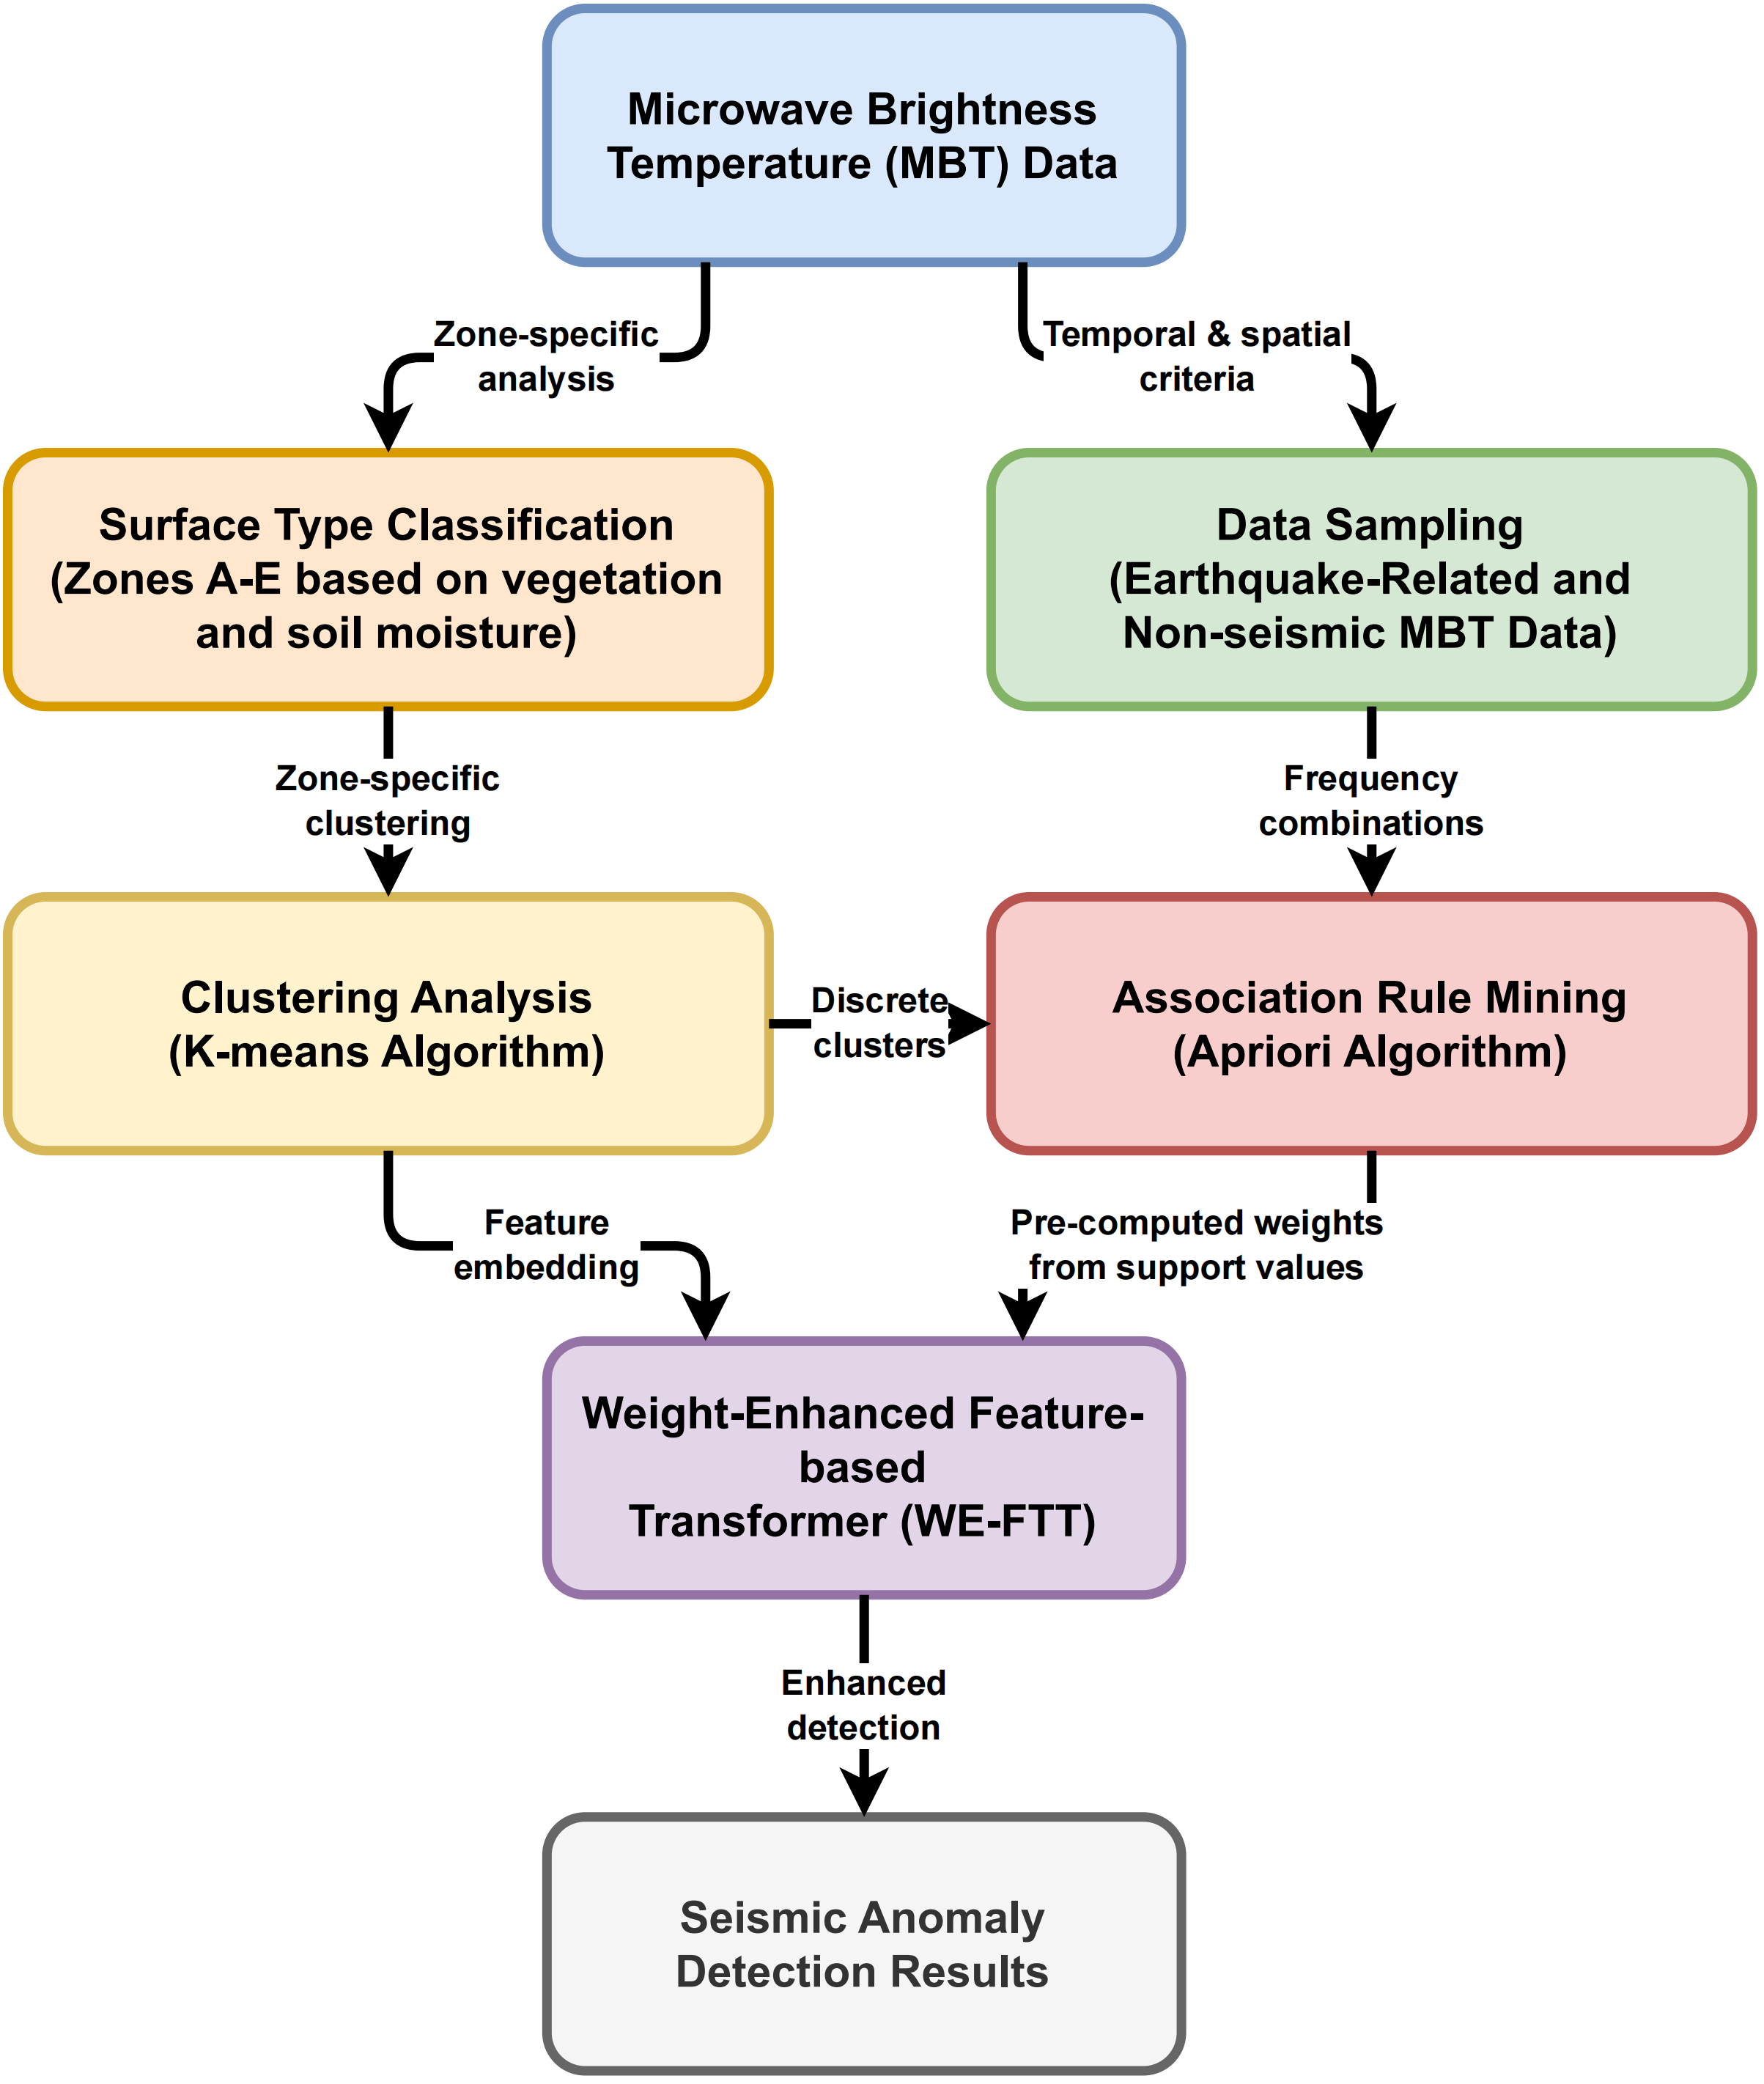
\includegraphics[width=1.0\linewidth]{image1.png}
\caption{Resolving signal ambiguity through environment-specific analysis: methodological framework. The workflow illustrates the integration of surface type classification, earthquake-related data sampling, clustering analysis, association rule mining, and the WE-FTT model.}\label{fig:fig1}
\end{figure*}
\clearpage

\begin{figure*}[!t]
\centering
\includegraphics[width=1.1\linewidth]{image11.png}
\caption{Global Distribution of Major Earthquakes (M$\ge$7.0) Across Different Surface Type Zones}\label{fig:fig11}
\end{figure*}
\clearpage

\begin{figure*}[p]
\centering
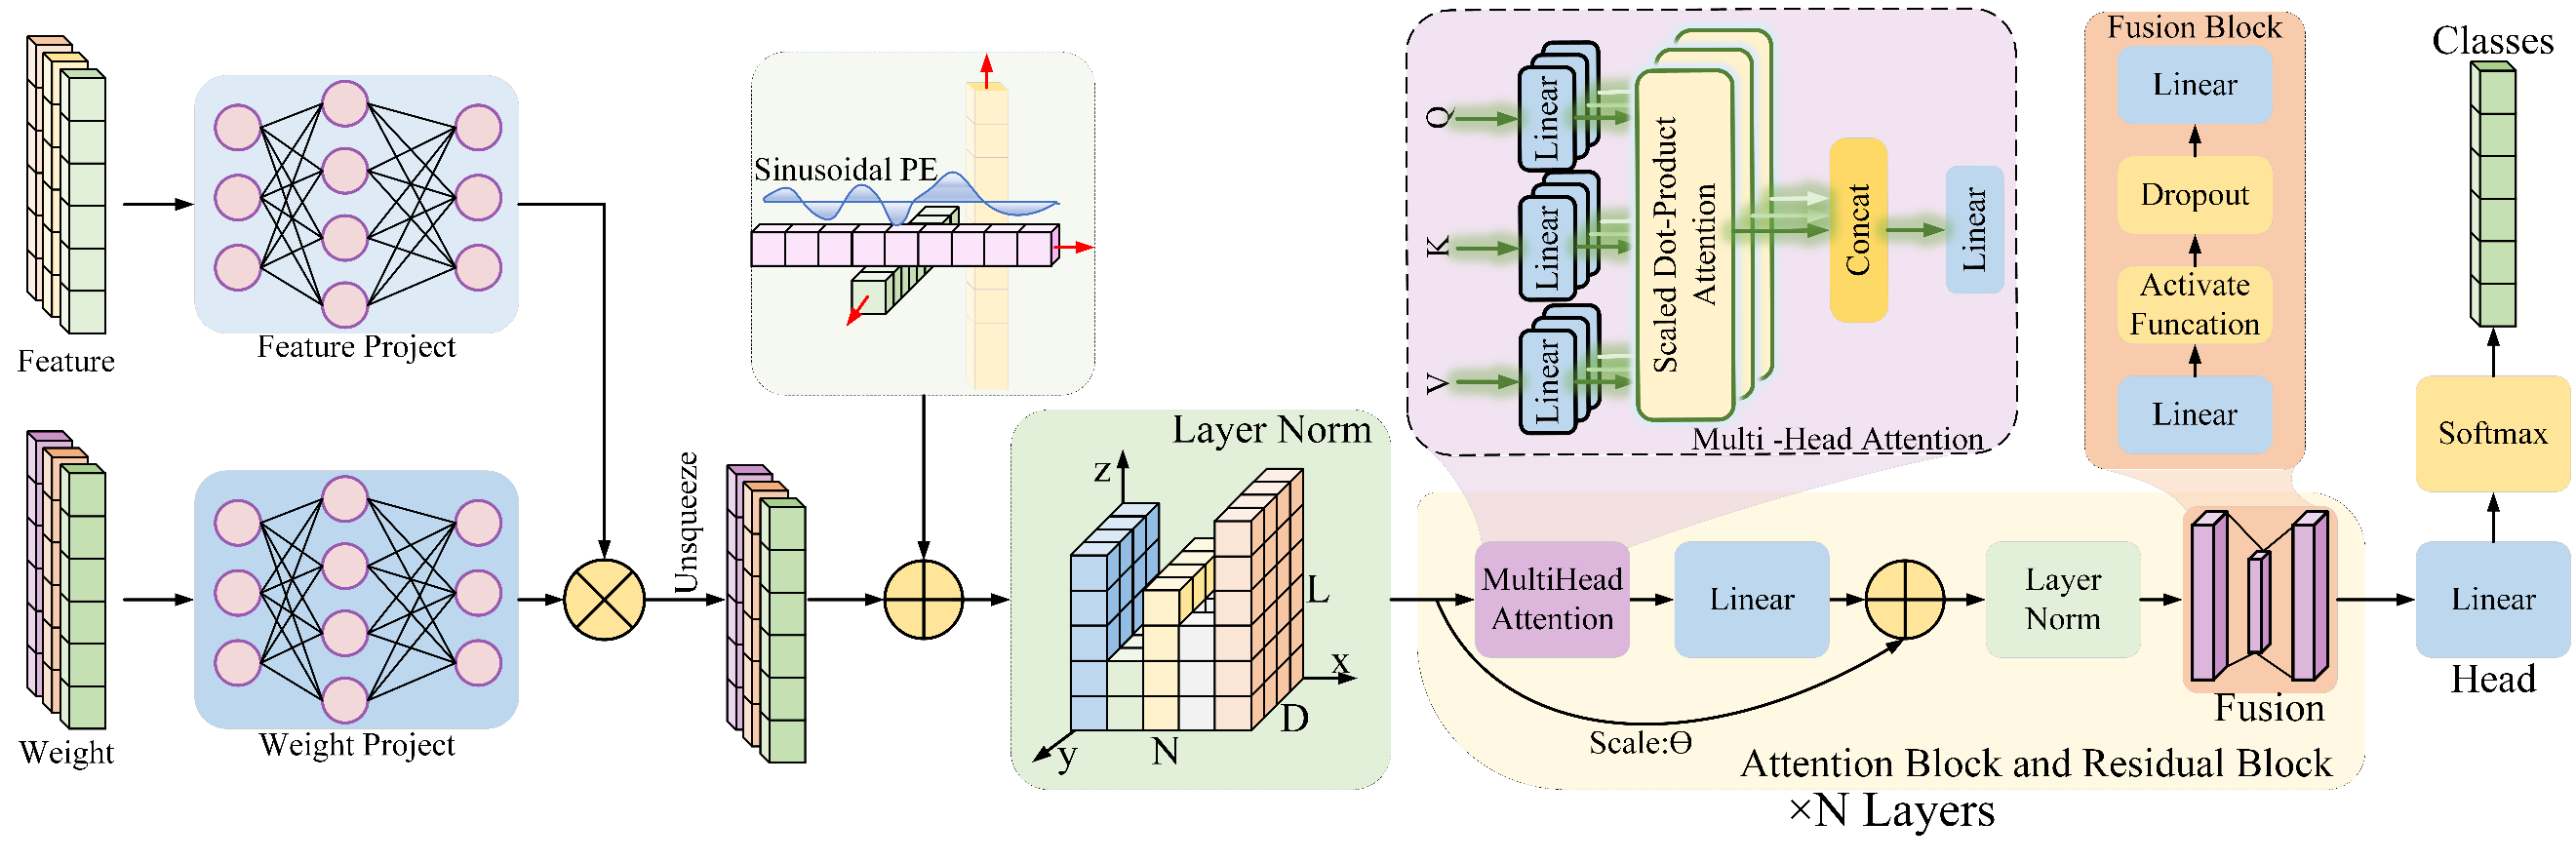
\includegraphics[width=1.1\linewidth]{image12.png}
\caption{Architectural overview of the WE-FTT.}\label{fig:fig12}
\end{figure*}
\clearpage

\begin{figure*}[p]
\centering
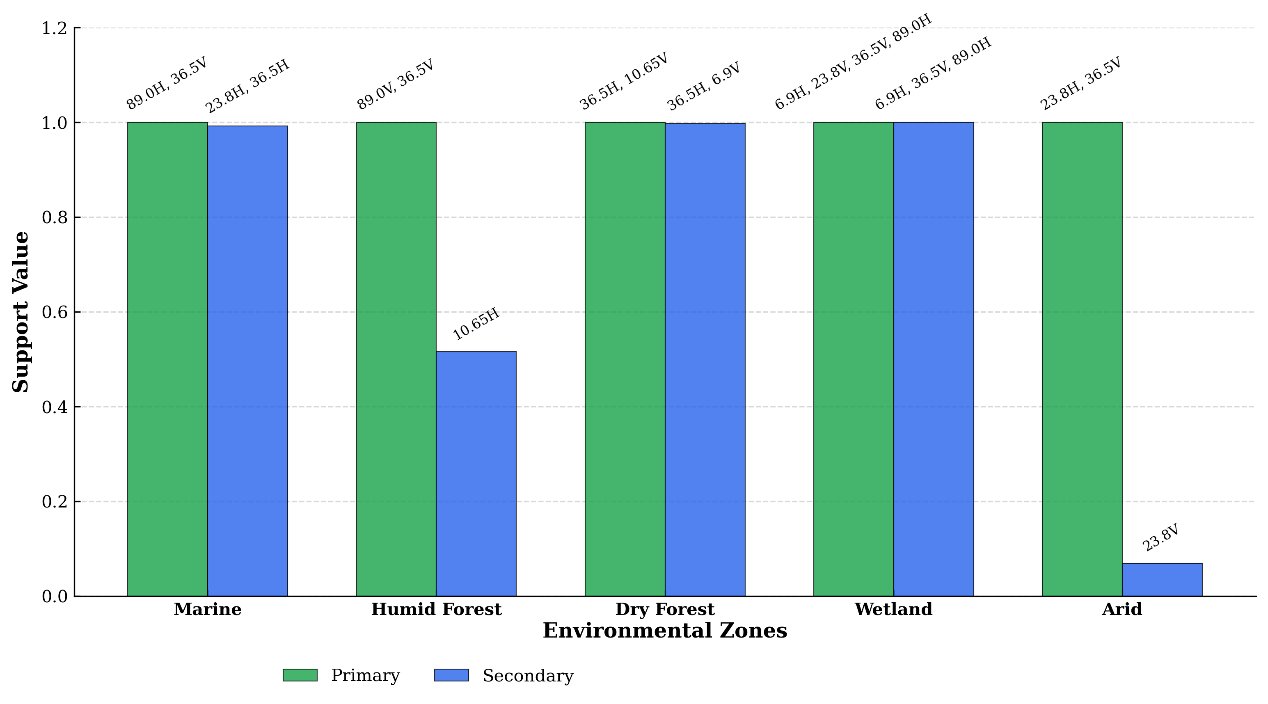
\includegraphics[width=1.0\linewidth]{image2.png}
\caption{Environment-specific frequency--polarization anomaly signatures with zone-dependent support.}\label{fig:fig2}
\end{figure*}
\clearpage

\begin{figure*}[p]
\centering
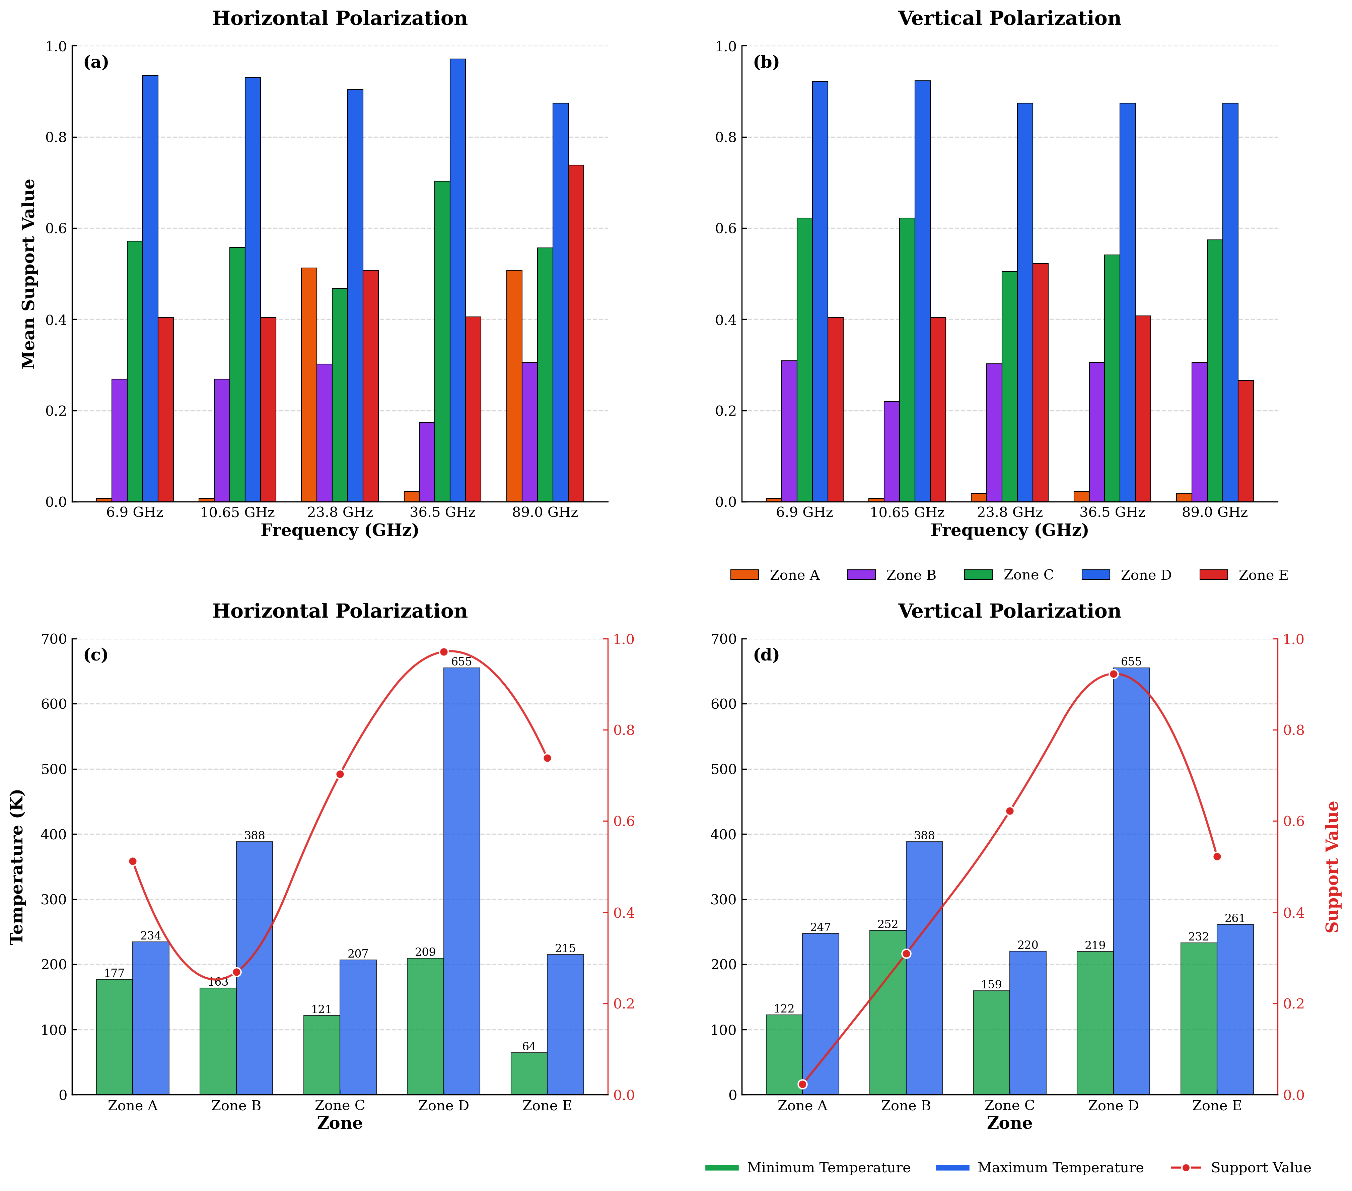
\includegraphics[width=1.1\linewidth]{image3.png}
\caption{Polarization dependence of microwave response characteristics across terrain zones.}\label{fig:fig3}
\end{figure*}
\clearpage

\begin{figure*}[p]
\centering
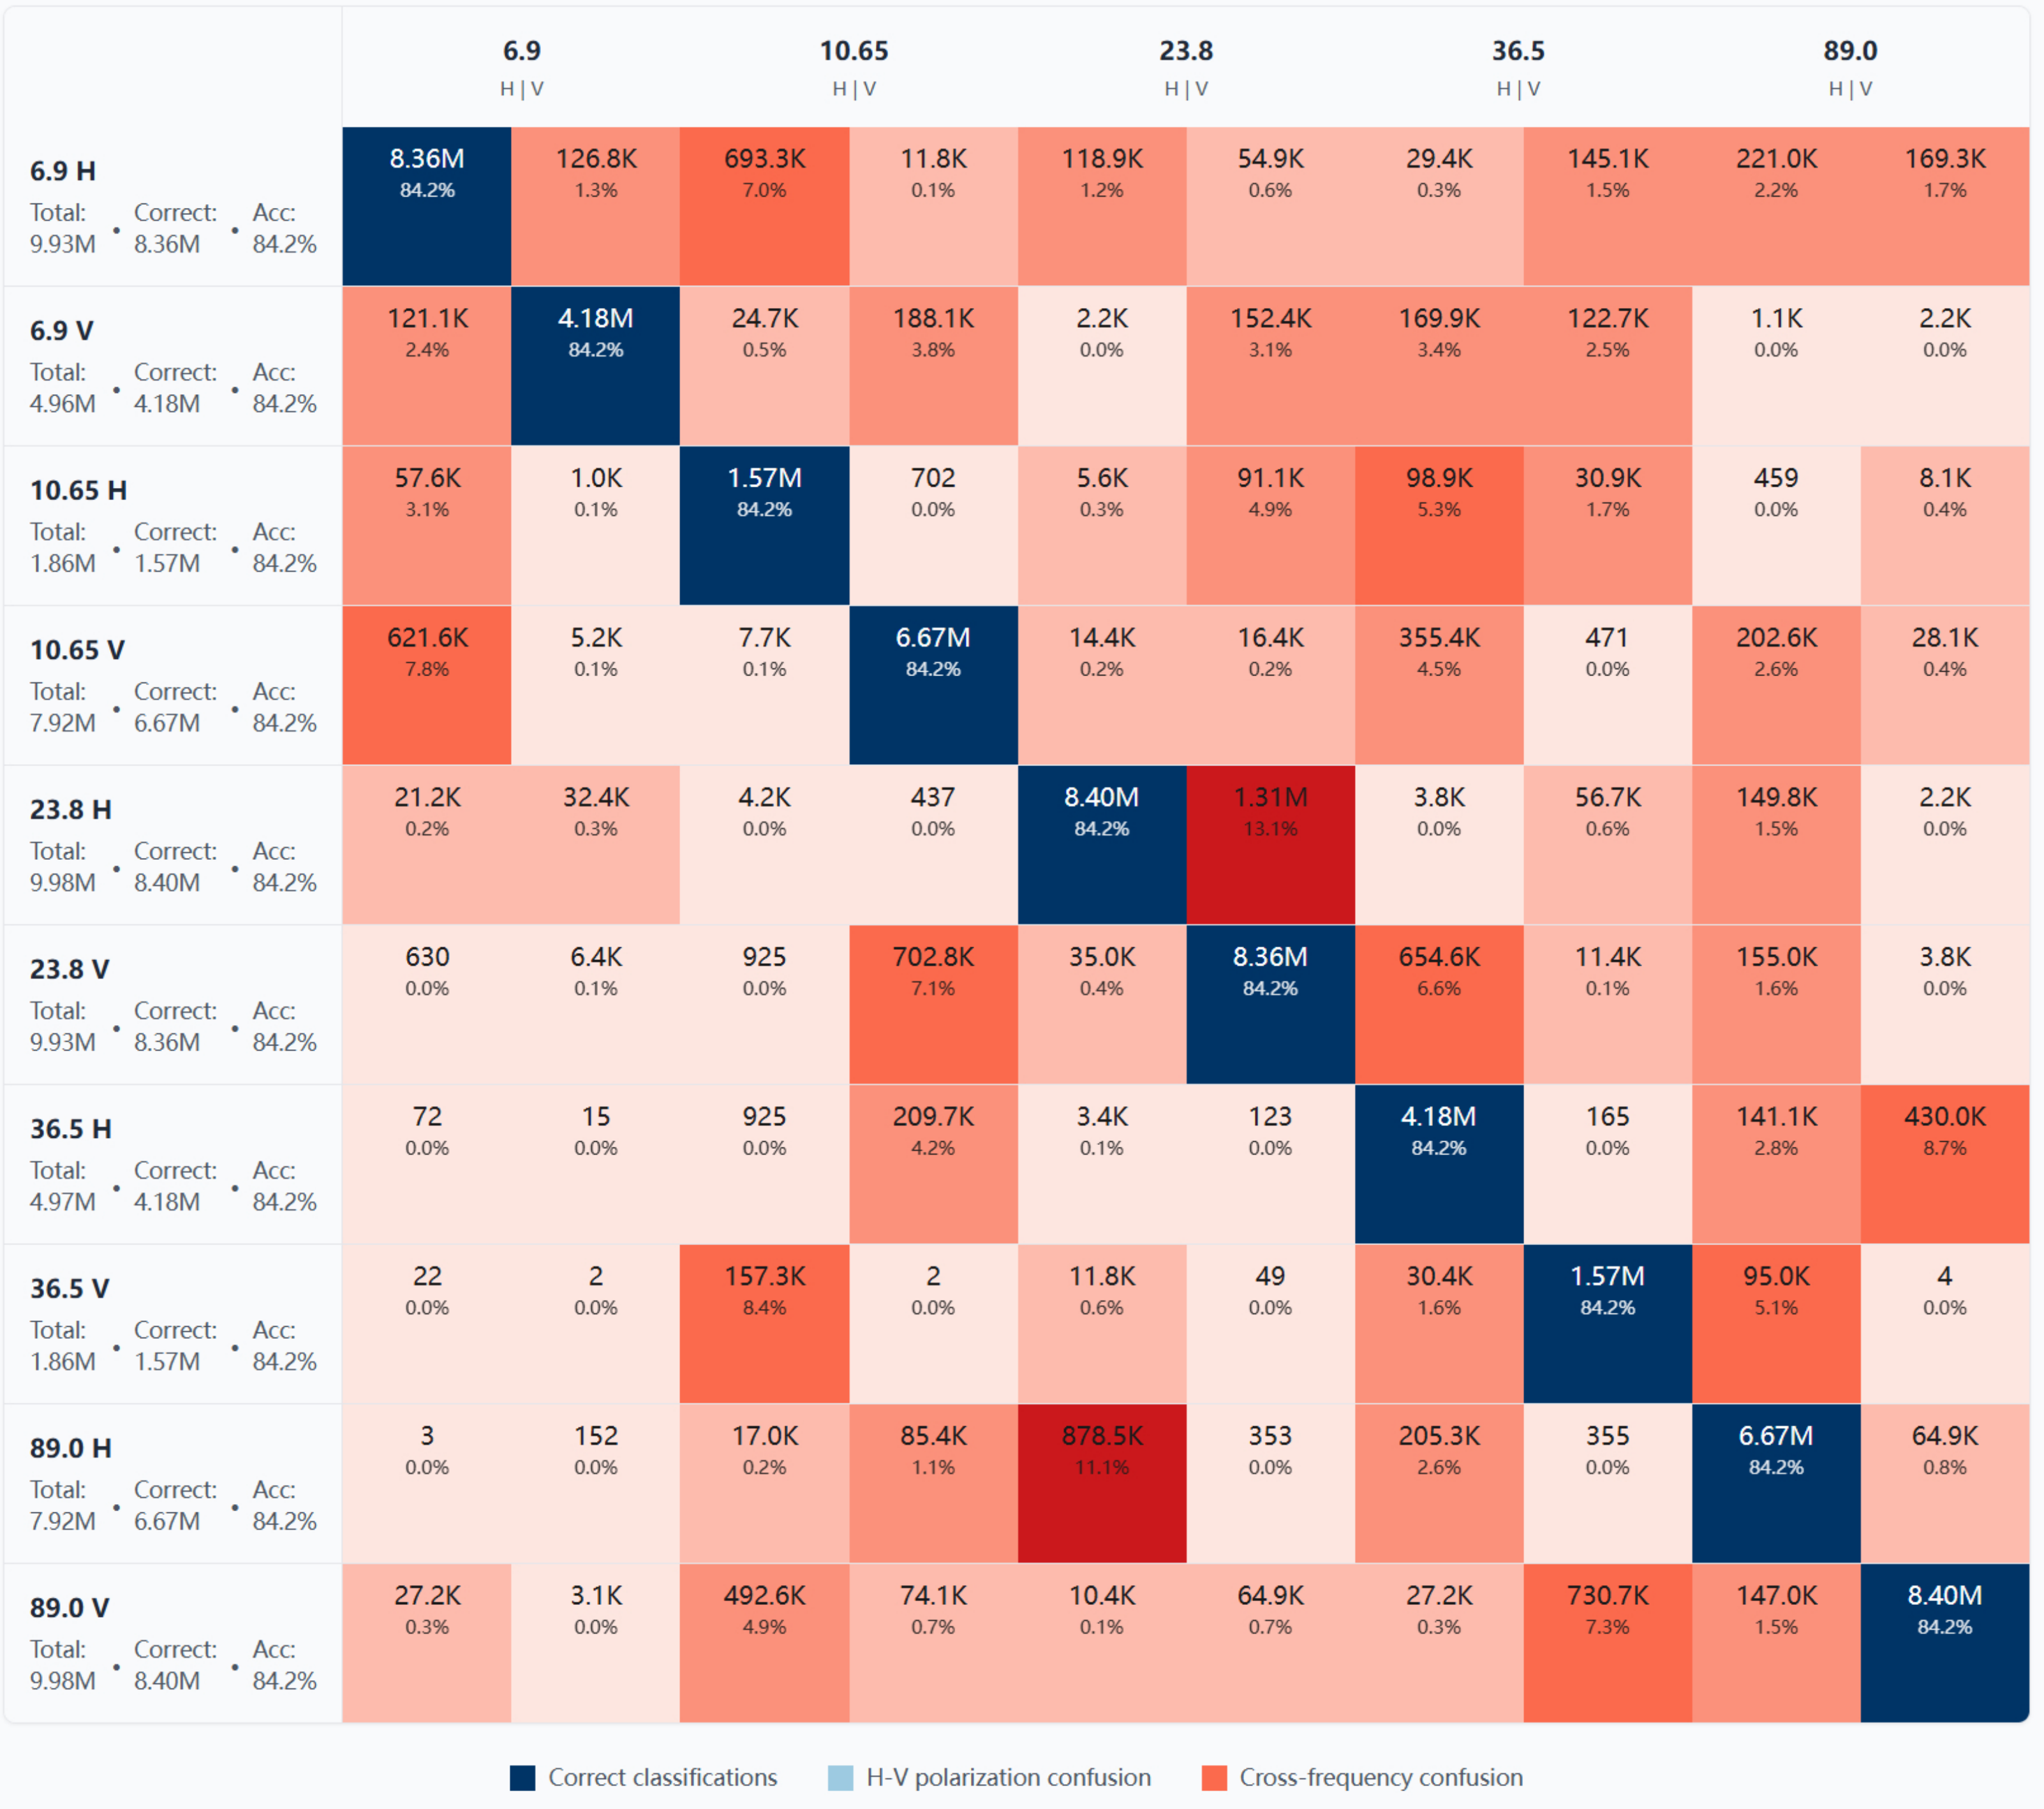
\includegraphics[width=1.1\linewidth]{image4.png}
\caption{Brightness Temperature Polarization Classification Matrix across five AMSR-2 frequency bands.}\label{fig:fig4}
\end{figure*}
\clearpage

\begin{figure*}[p]
\centering
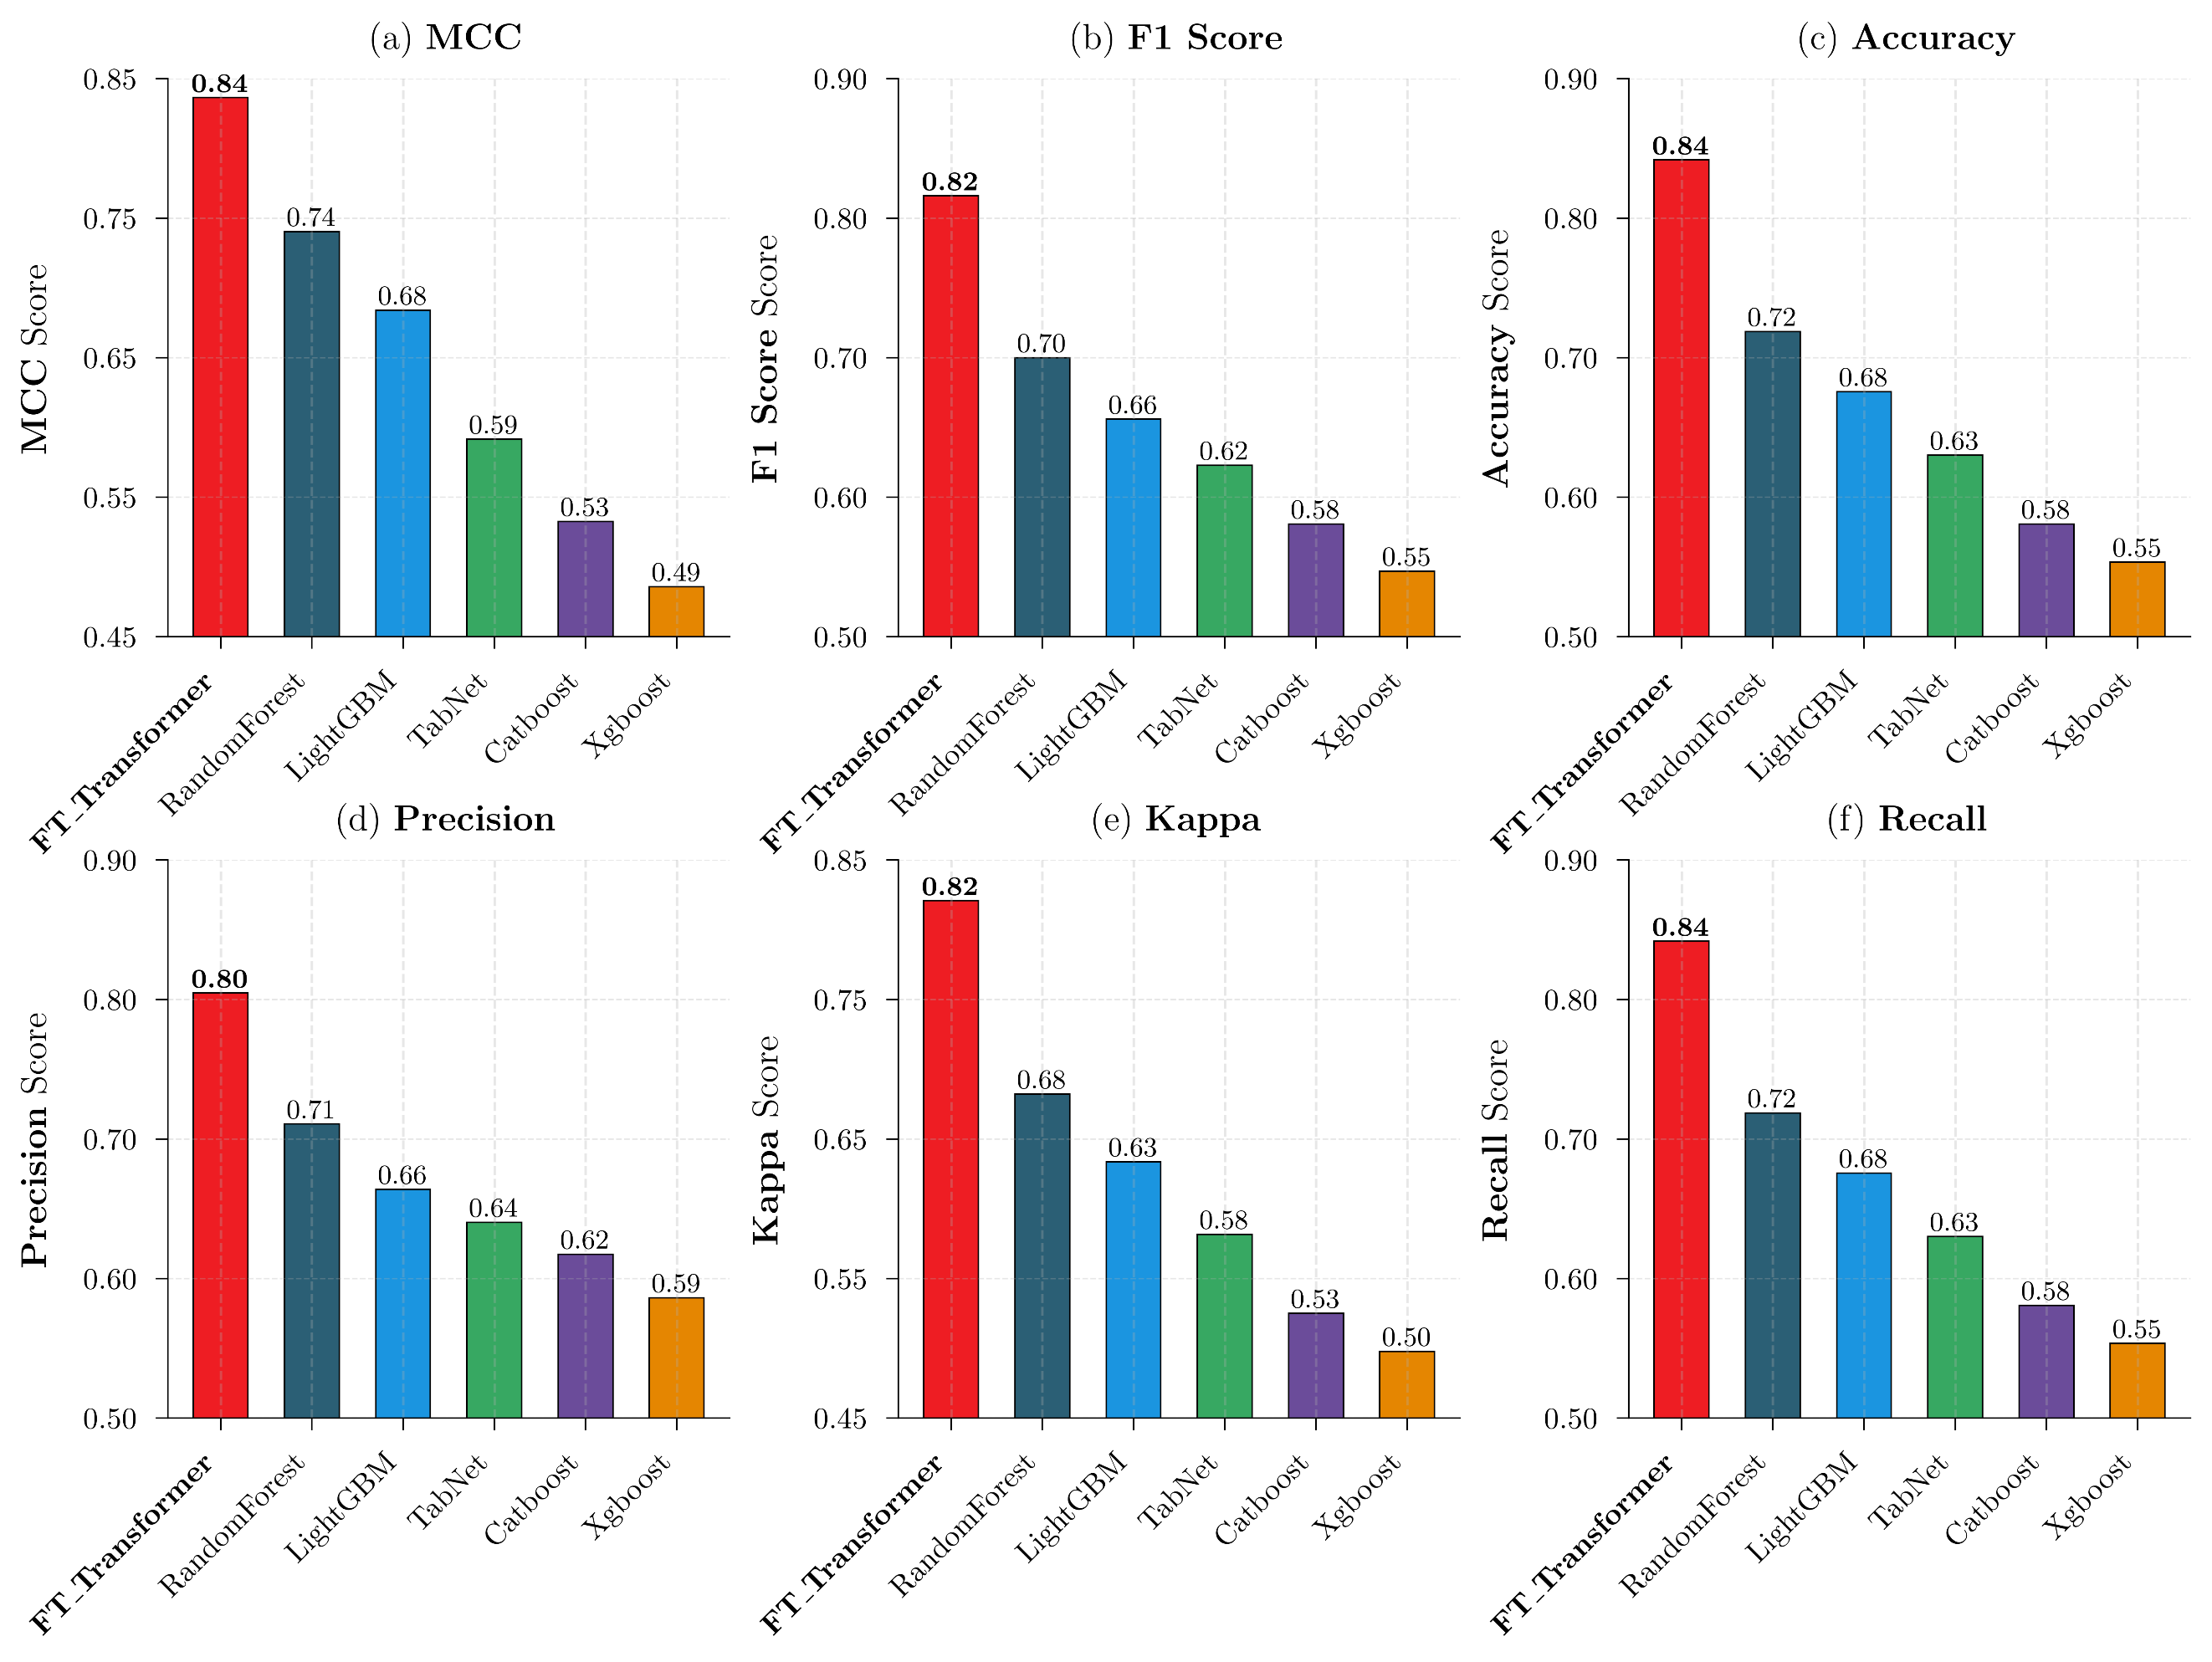
\includegraphics[width=1.1\linewidth]{image5.png}
\caption{Model performance comparison across six evaluation metrics.}\label{fig:fig5}
\end{figure*}
\clearpage

\begin{figure*}[p]
\centering
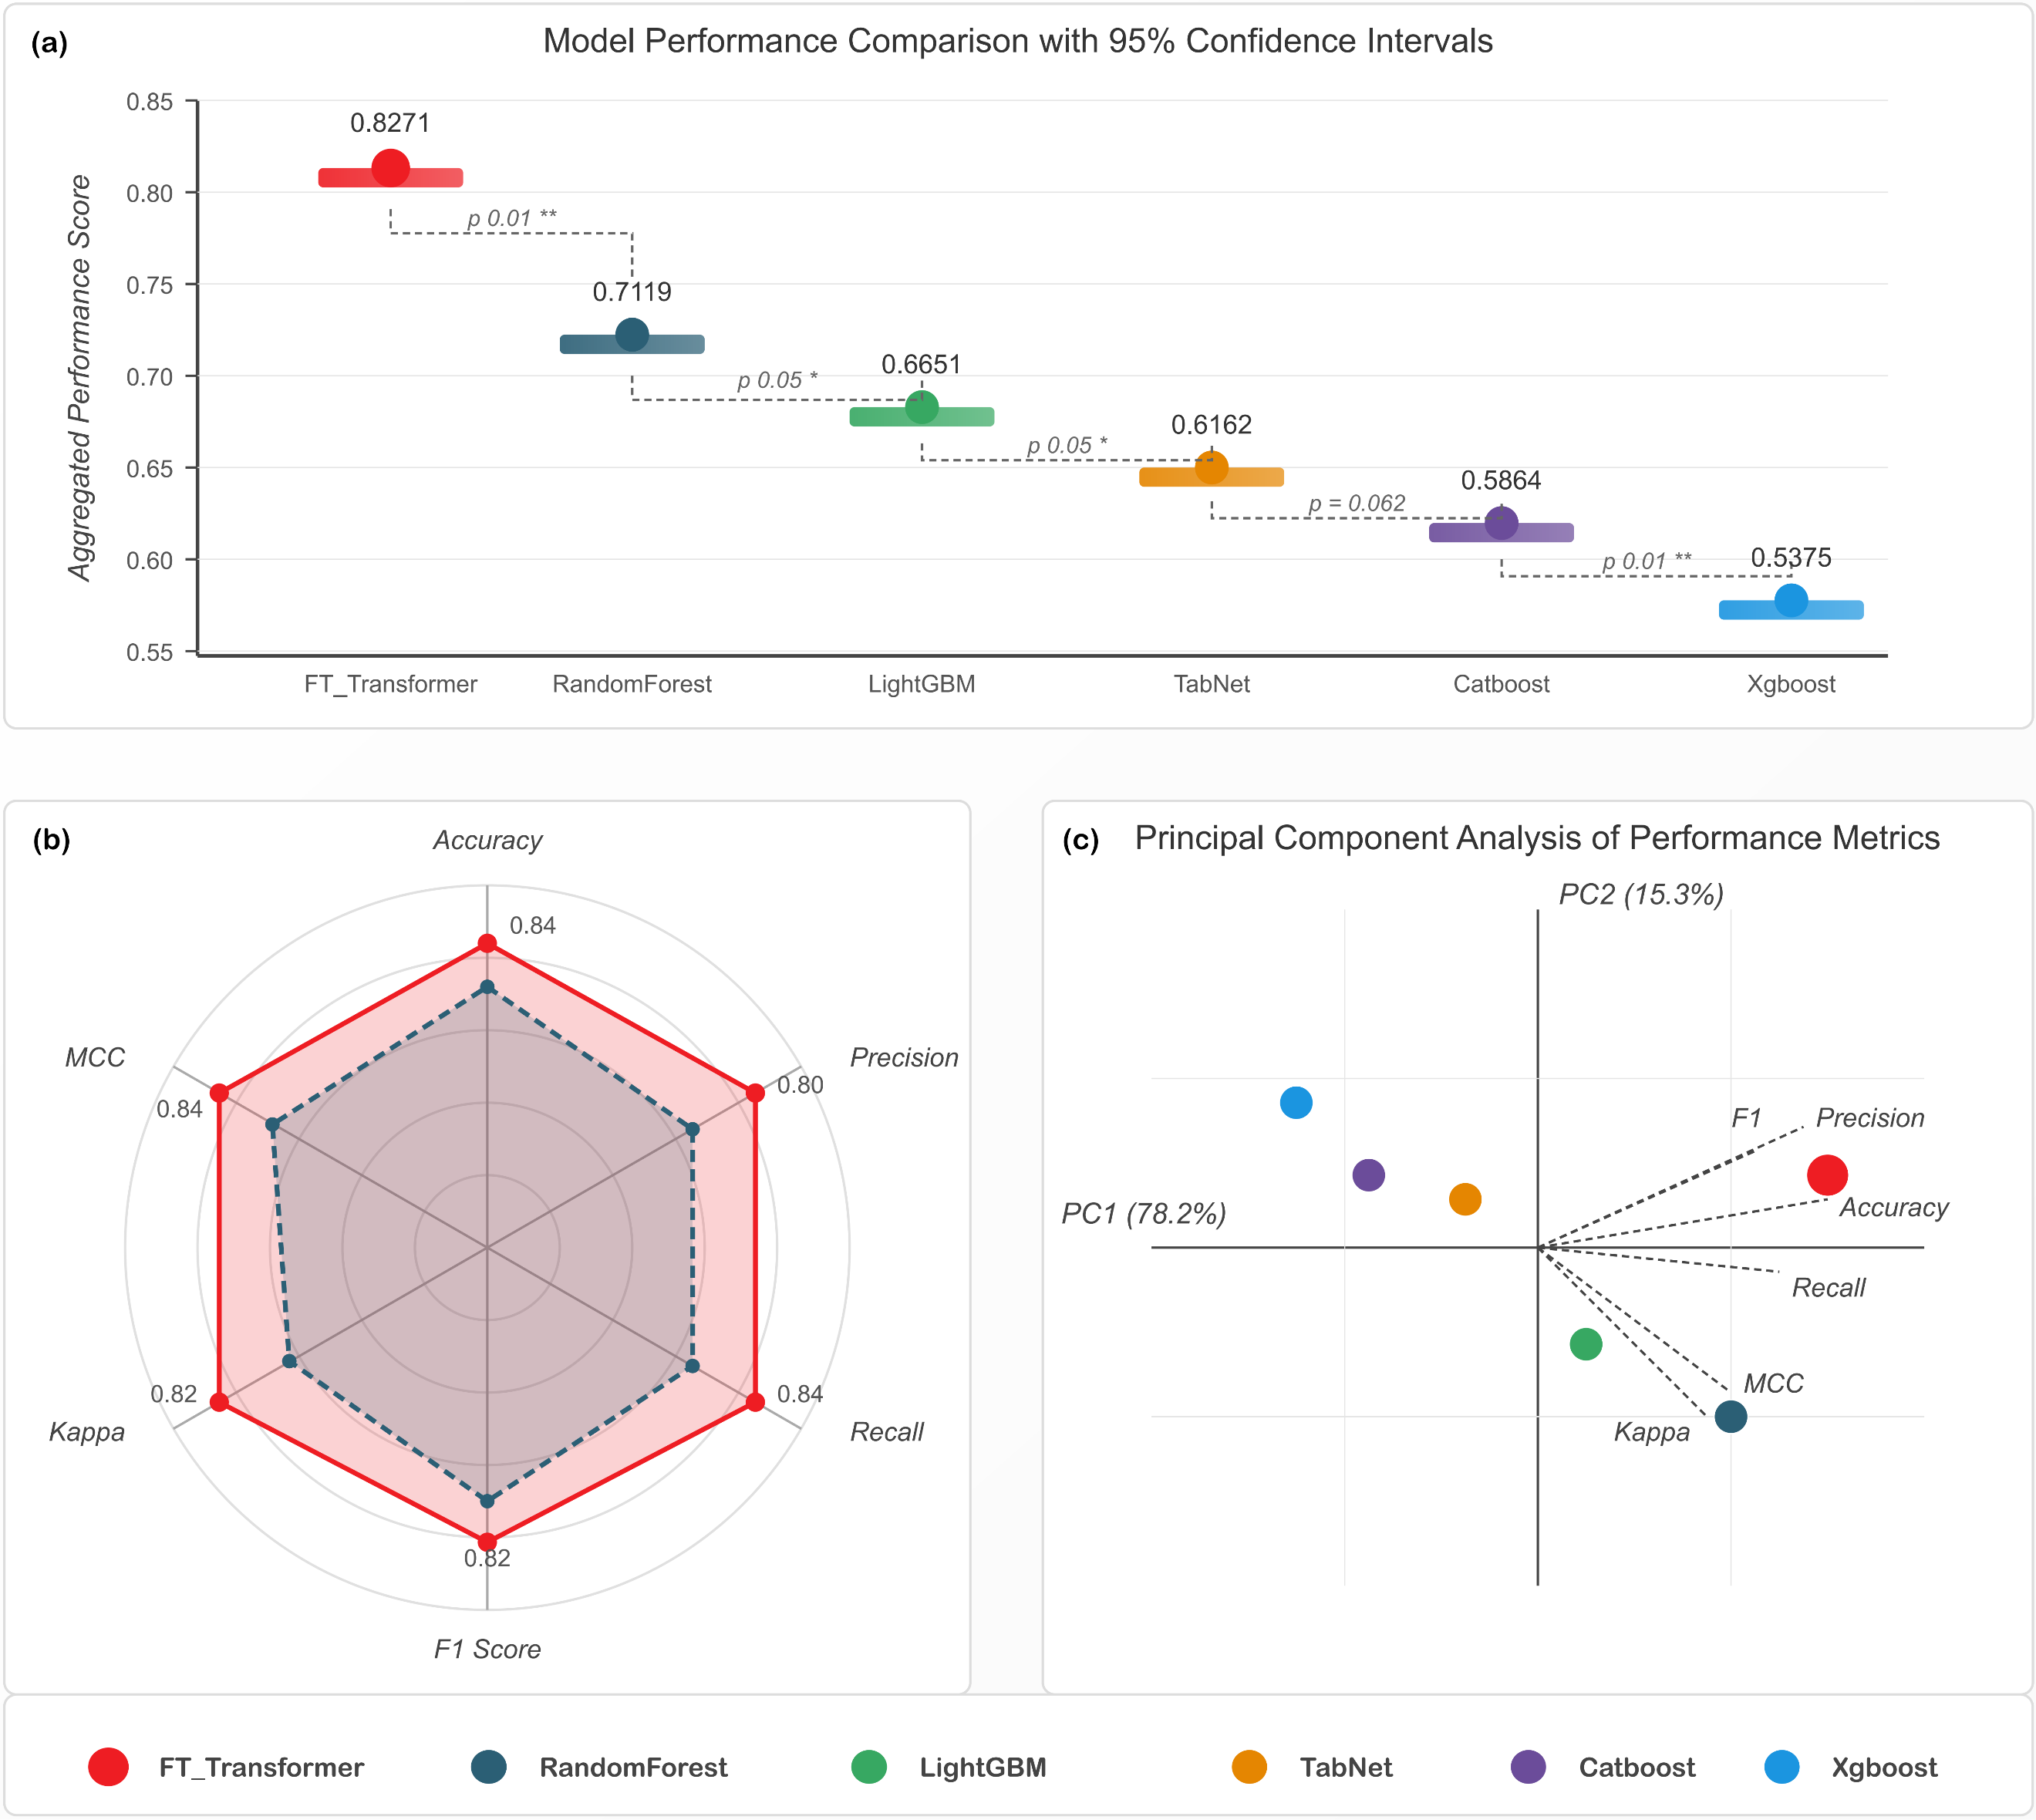
\includegraphics[width=1.1\linewidth]{image6.png}
\caption{Comprehensive model performance analysis with PCA-based visualization of metric relationships. PCA is used here solely for visualization and is not treated as a predictive baseline.}\label{fig:fig6}
\end{figure*}
\clearpage

\begin{figure*}[p]
\centering
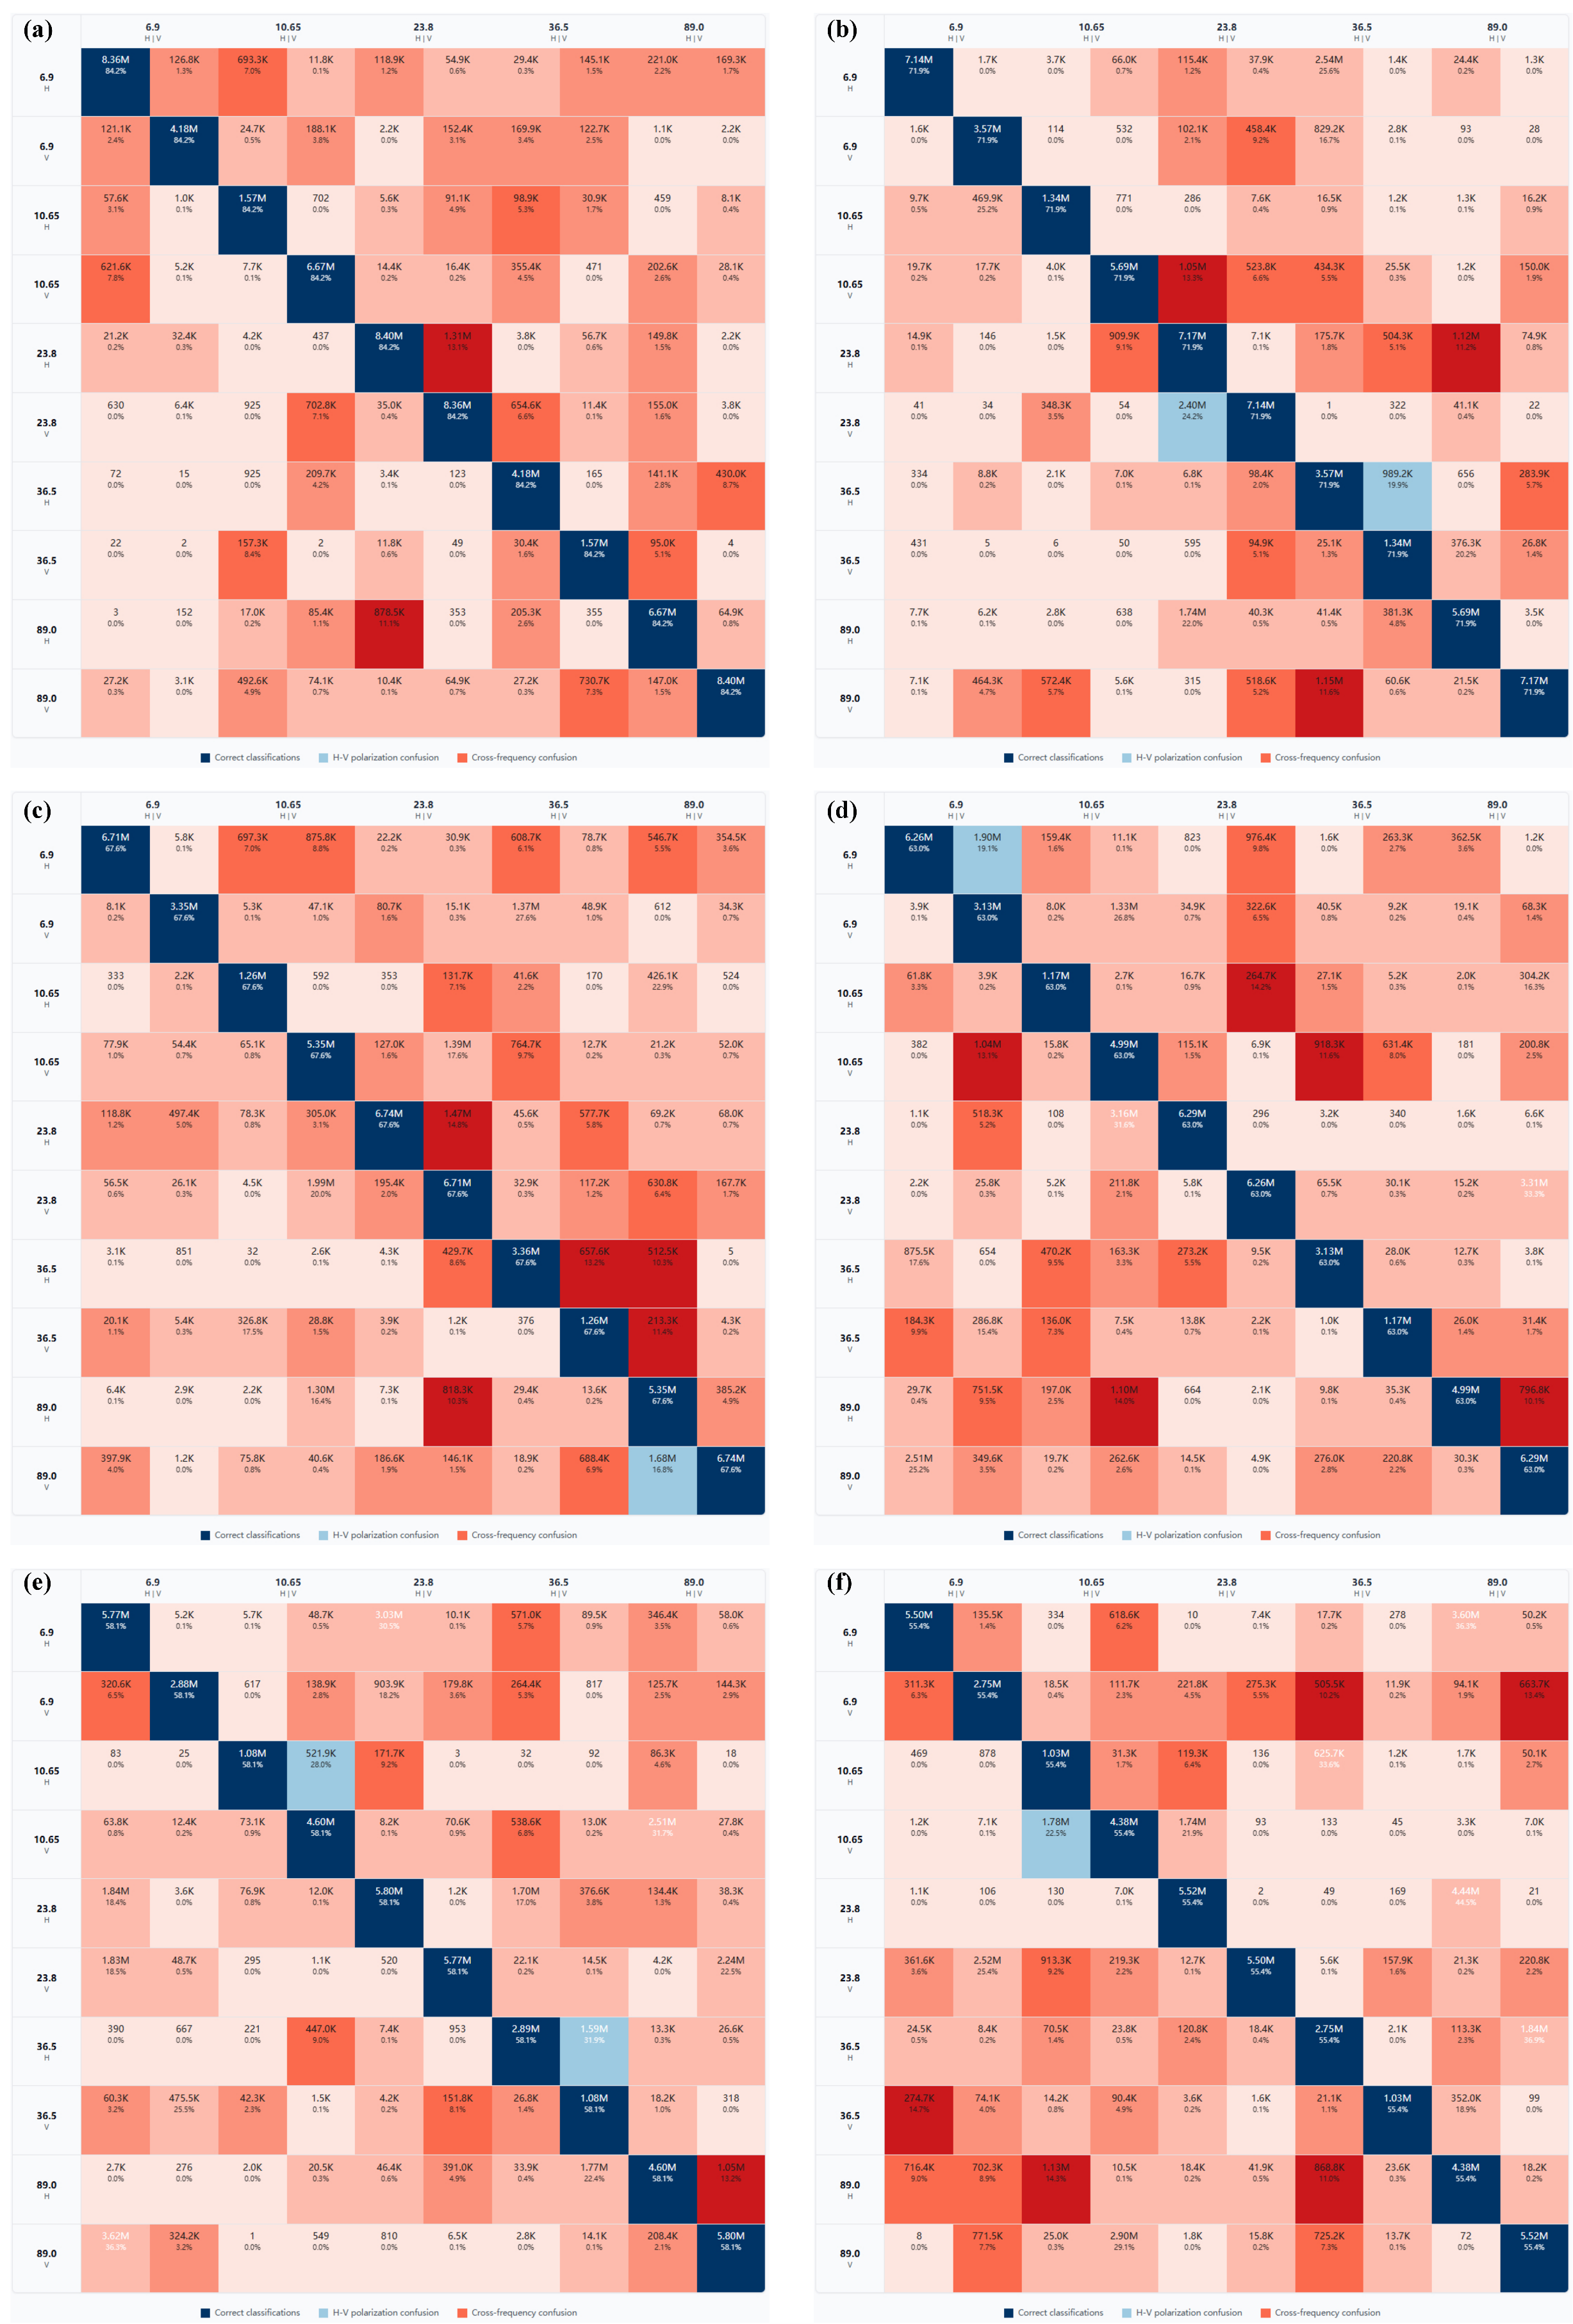
\includegraphics[width=1.0\linewidth]{image7.png}
\caption{Confusion matrices showing classification performance across different models.}\label{fig:fig7}
\end{figure*}
\clearpage

\begin{figure*}[p]
\centering
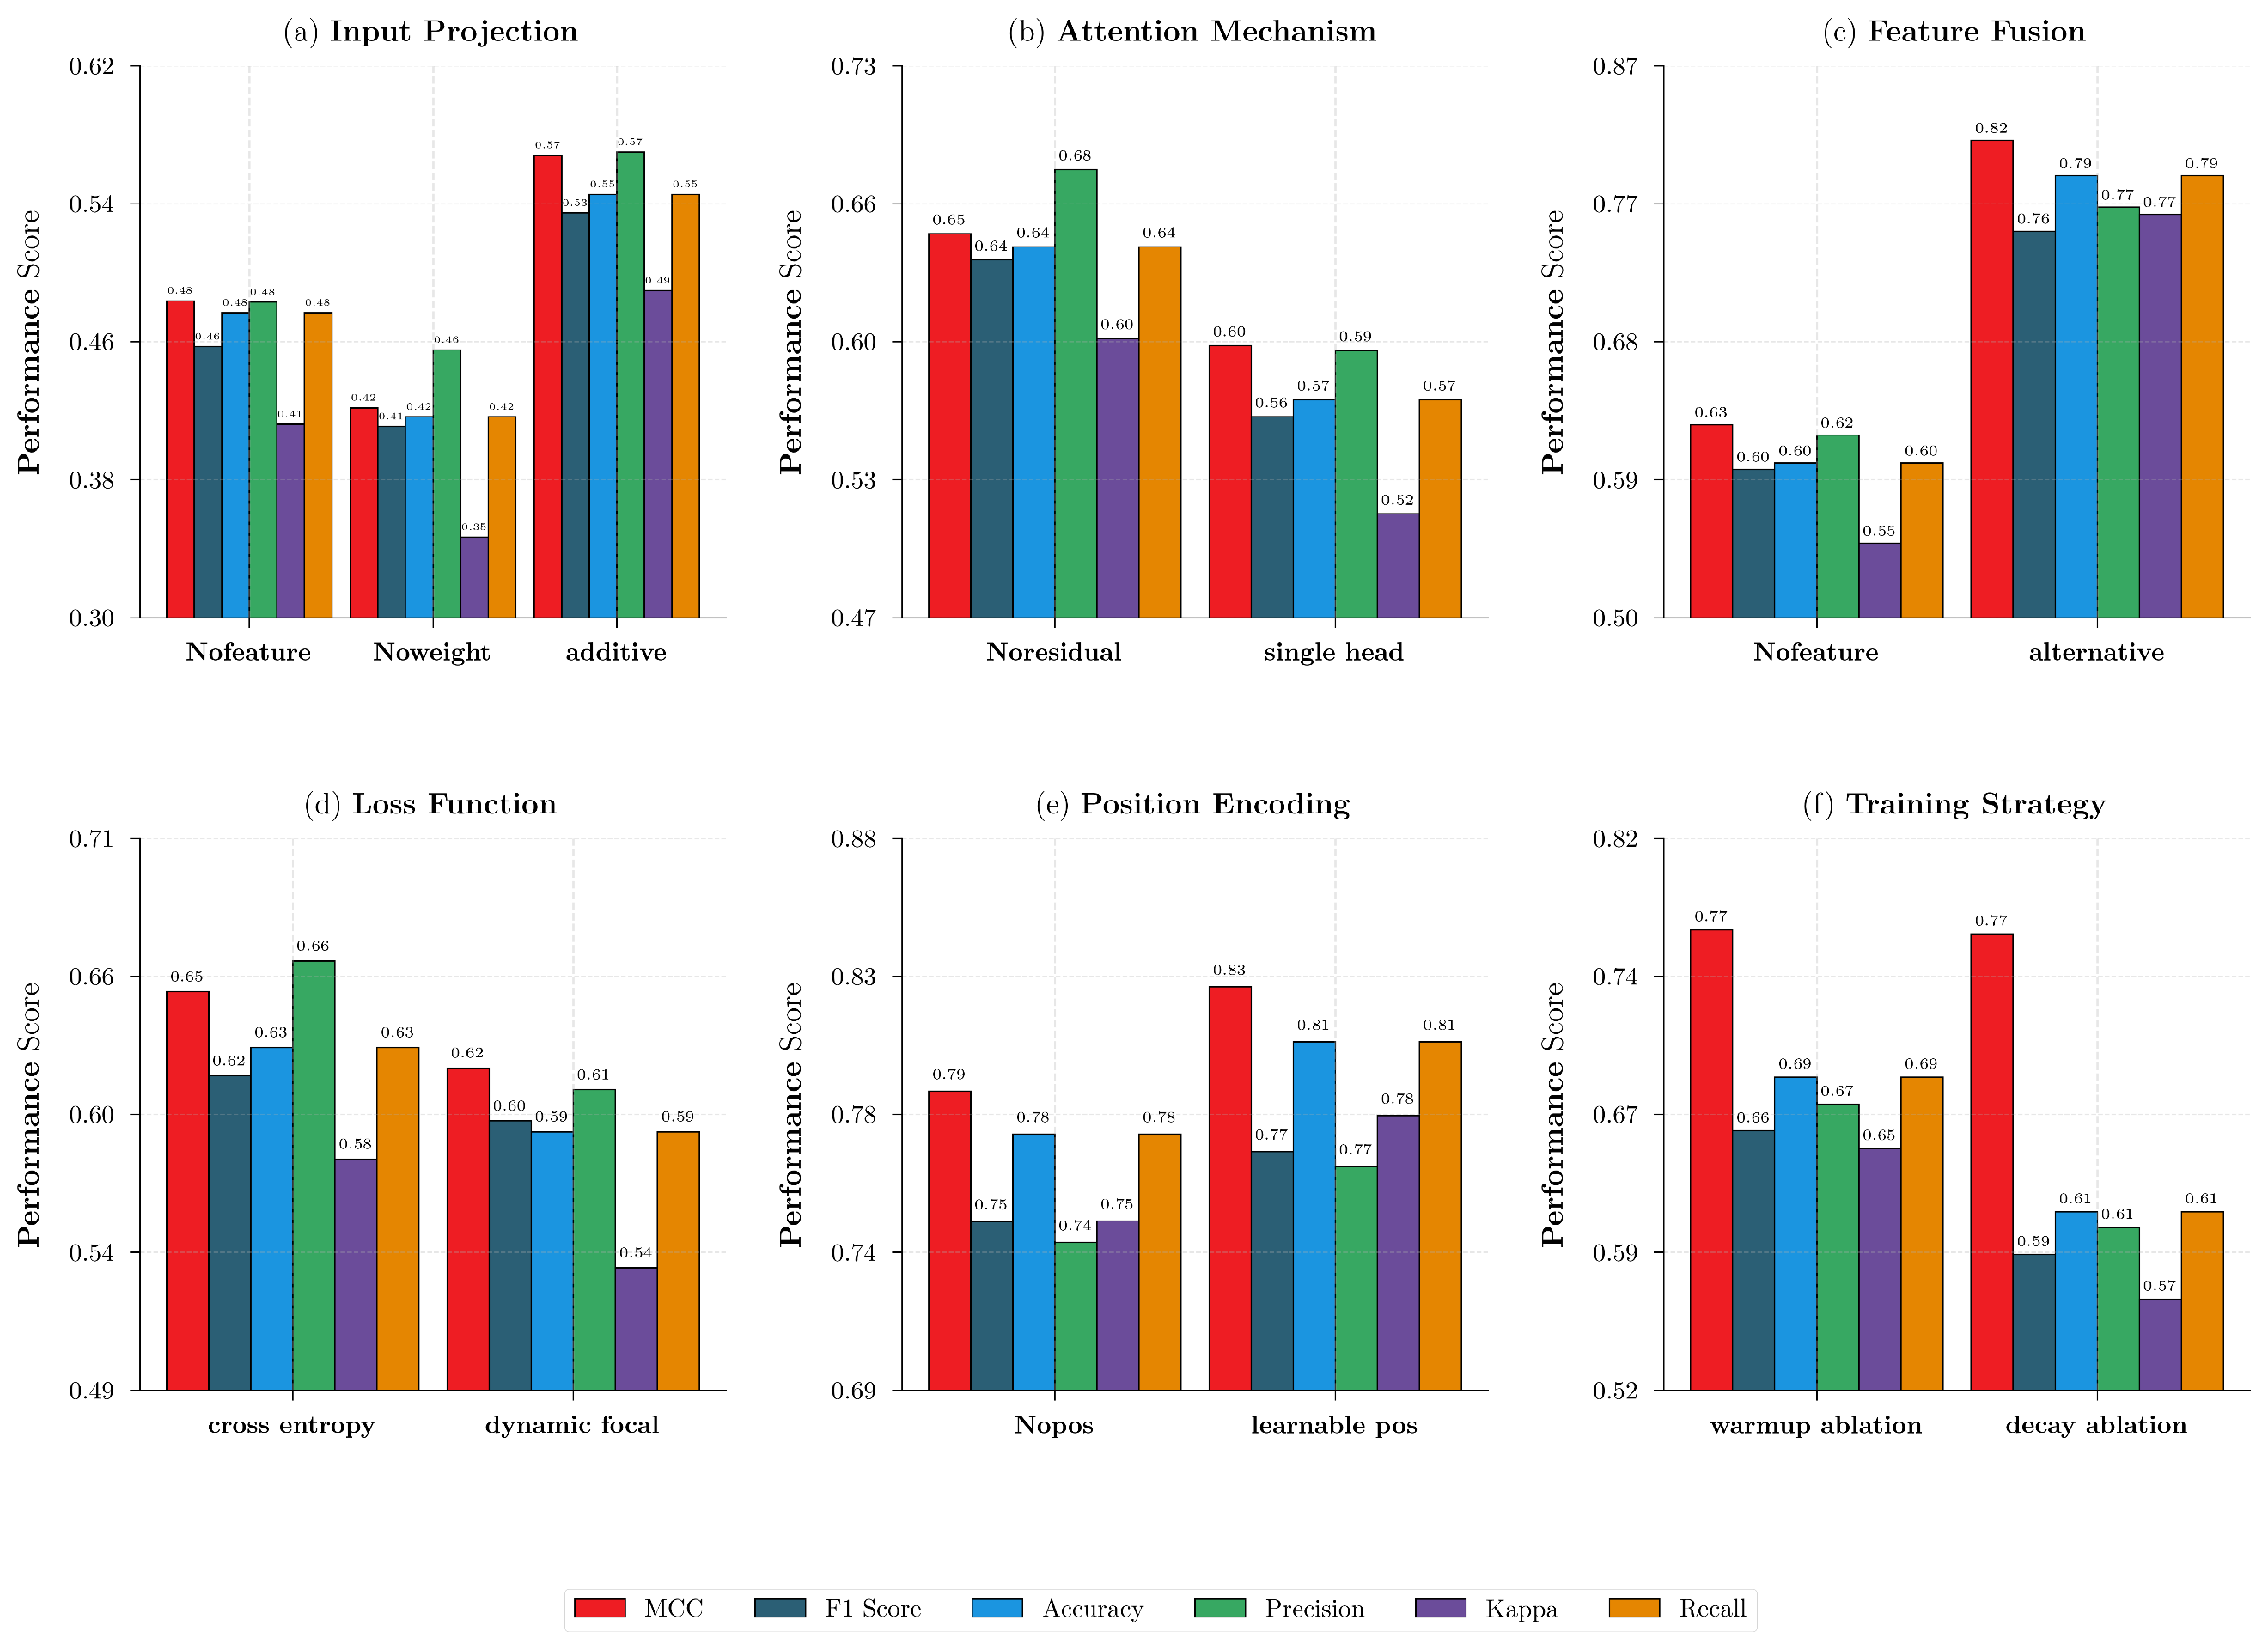
\includegraphics[width=1.1\linewidth]{image8.png}
\caption{Ablation study results across key architectural components.}\label{fig:fig8}
\end{figure*}
\clearpage

\begin{figure*}[p]
\centering
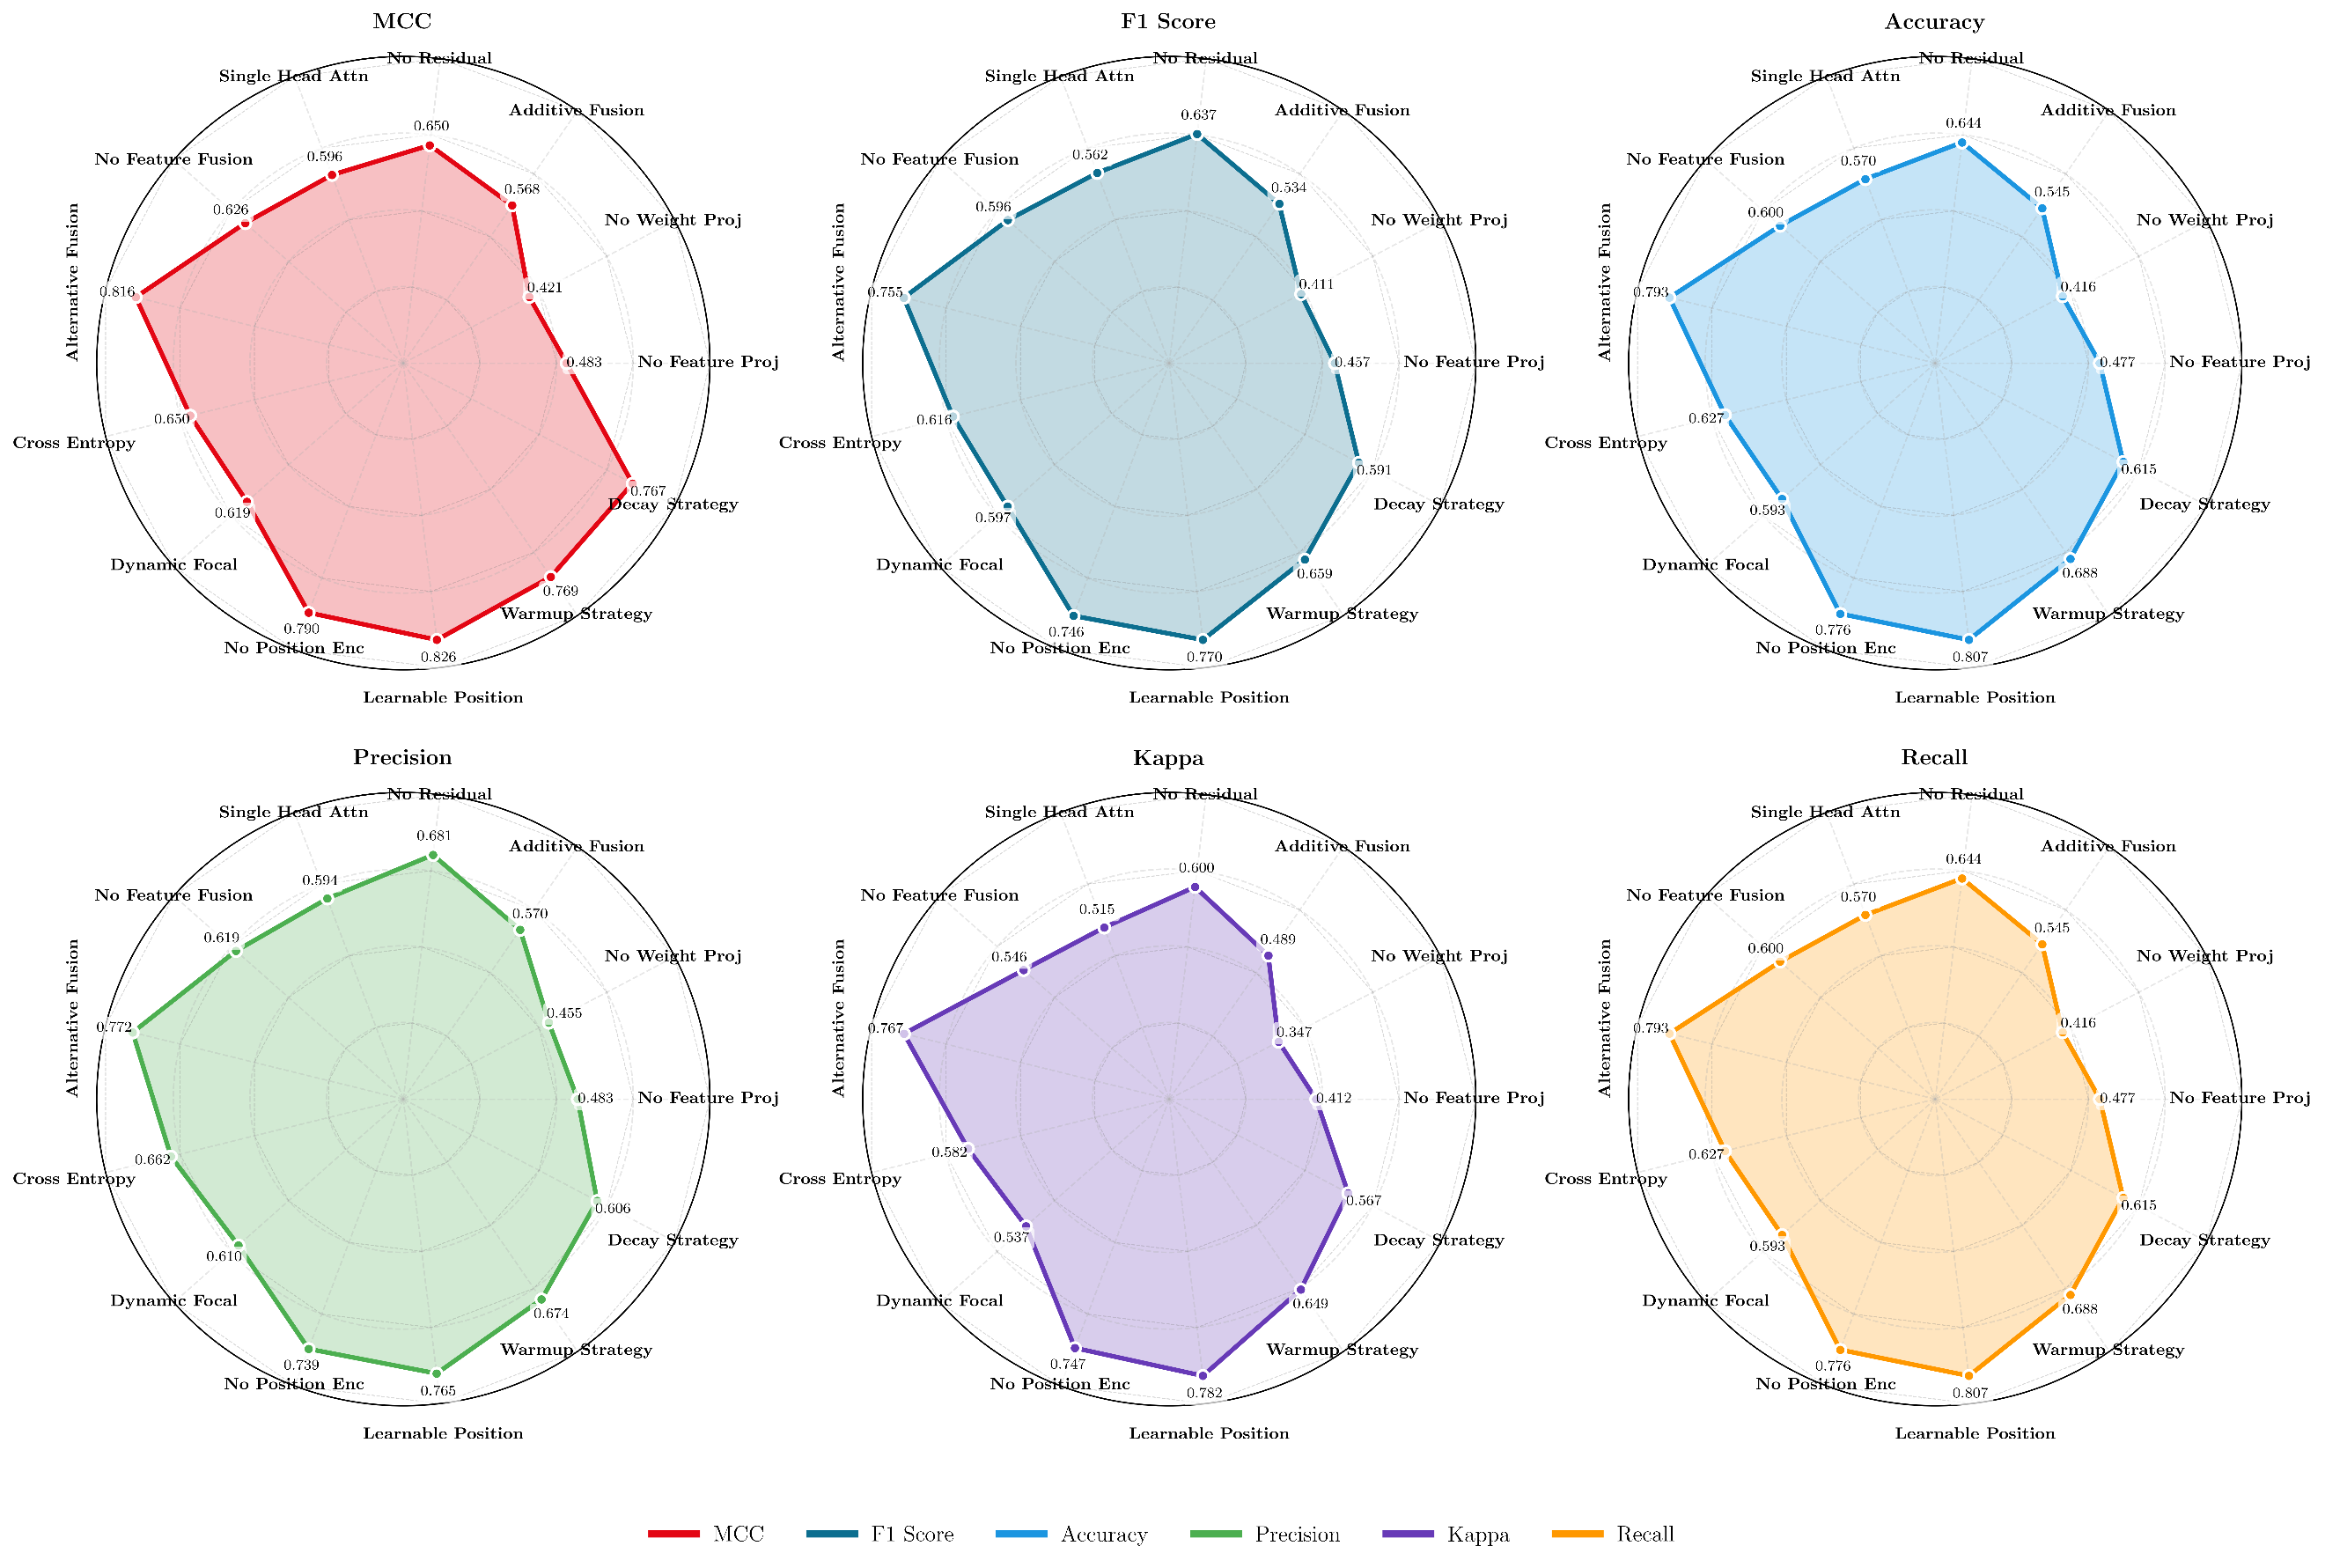
\includegraphics[width=1.1\linewidth]{image9.png}
\caption{Radar visualization of model performance metrics across ablation variants.}\label{fig:fig9}
\end{figure*}
\clearpage

\begin{figure*}[p]
\centering
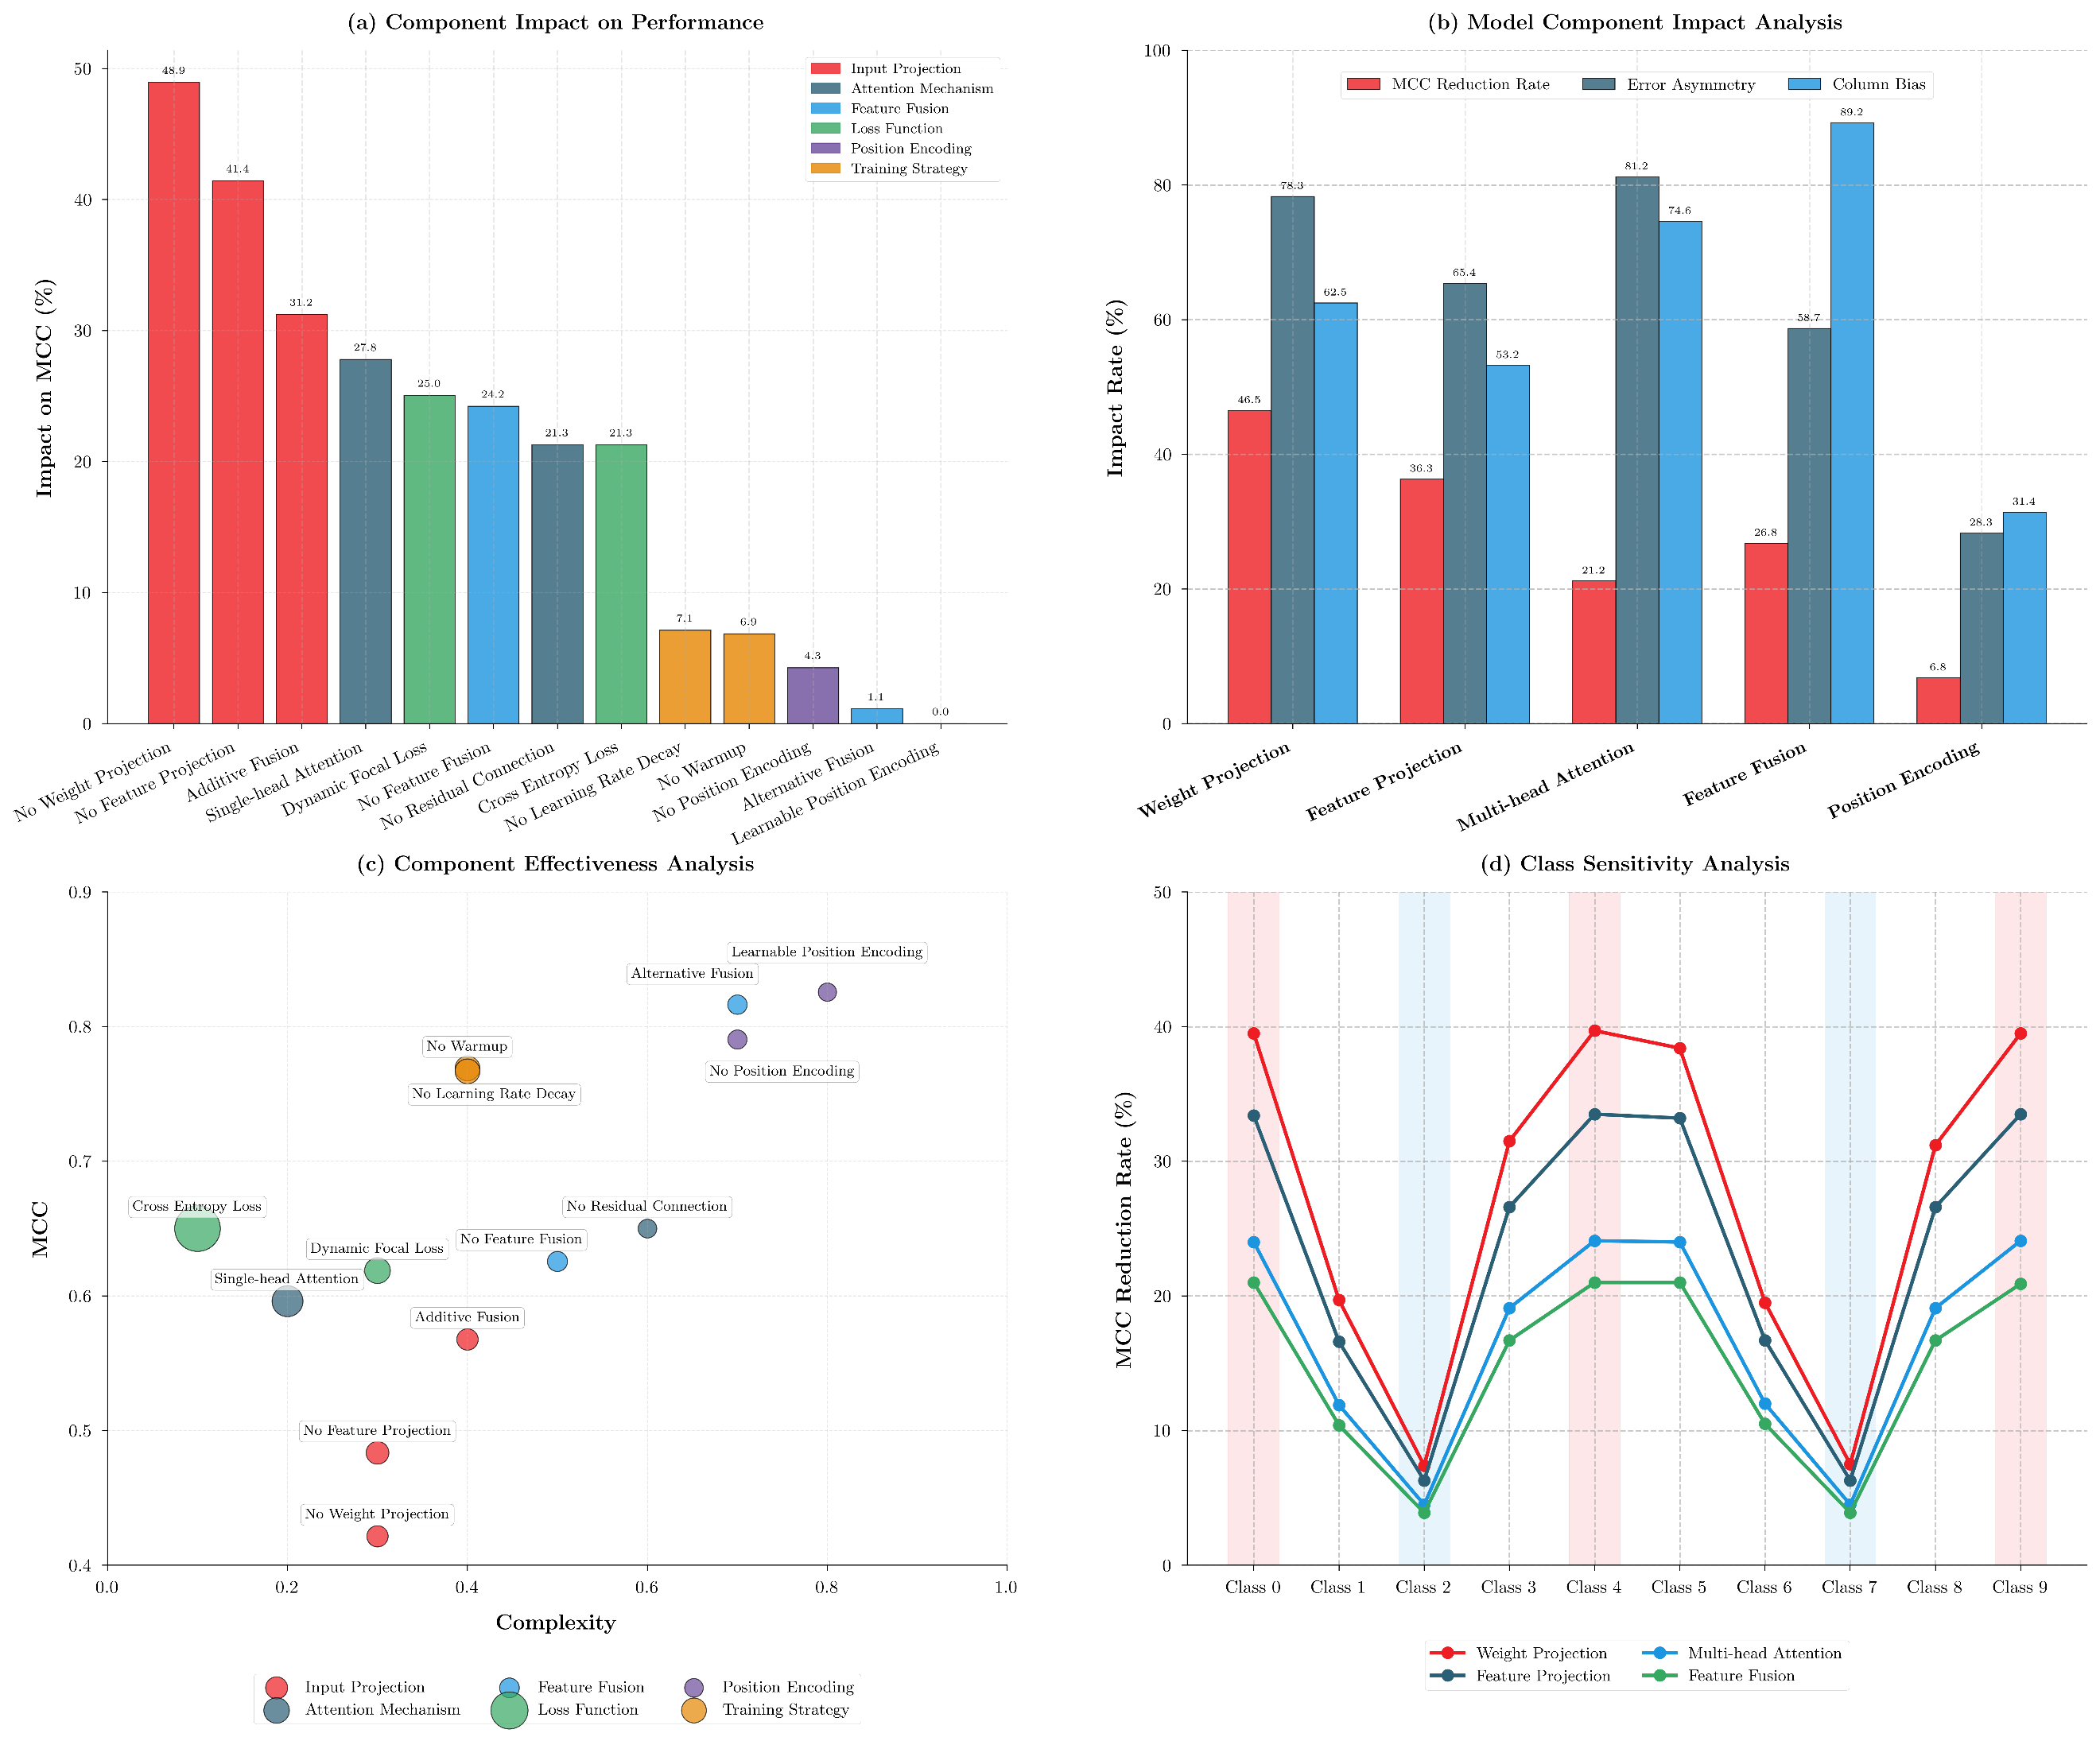
\includegraphics[width=1.1\linewidth]{image10.png}
\caption{Comprehensive ablation analysis of the WE-FTT model.}\label{fig:fig10}
\end{figure*}
\clearpage

\begin{figure*}[p]
\centering
\includegraphics[width=1.1\linewidth]{fig_13_global_fpr.pdf}
\caption{Global per-pixel false-positive rates (FPR) on randomly sampled non-seismic days, aggregated to 1$^{\circ}$ for visualization. Marine regions (Zone~A) exhibit higher median FPR (0.242) than inland environmental zones (B--E; medians 0.083, 0.125, 0.033, and 0.100, respectively), consistent with Supplementary Table~\ref{tab:tableS1} and highlighting the efficacy of environment-specific thresholds over land.}\label{fig:fig13}
\end{figure*}
\clearpage


% ===== Tables =====
\clearpage
\begin{table*}[p]
\small
\centering
\caption{Segmented MBT ranges and mean support values across terrain zones. Note: 655.35~K denotes the AMSR-2 fill-value upper bound; all pixels with this value were removed during preprocessing and do not contribute to any of the reported statistics.}\label{tab:table1}
\resizebox{\textwidth}{!}{%
 \renewcommand{\arraystretch}{1.1}
\begin{tabular}{@{}llccccc@{}}
\toprule
      &   & \multicolumn{5}{c}{Mean Support Value (MBT segmentation range)} \\
 \cmidrule(lr){3-7}
\multicolumn{2}{l}{Freq. (GHz)}  & Zone A & Zone B & Zone C & Zone D & Zone E \\
\midrule
\multirow{4}{*}{6.9}
    & \multirow{2}{*}{H}
        & 0.0074\,(41.8--168.1)  & 0.2688\,(163.7--388.2) & 0.5716\,(73.6--145.6)  & 0.9348\,(166.4--655.4) & 0.4038\,(168.9--655.4) \\
    &   & ---                   & 0.2201\,(73.4--163.7)  & 0.4408\,(226.8--382.8) & 0.8015\,(73.3--166.4)  & 0.0042\,(14.3--168.9) \\[6pt]
    & \multirow{2}{*}{V}
        & 0.0076\,(57.1--219.2)  & \textbf{0.3095\,(252.2--388.1)} & 0.6219\,(152.3--215.6) & 0.9219\,(214.9--655.4) & 0.4038\,(218.6--655.4) \\
    &   & ---                   & 0.2193\,(138.1--205.0) & 0.4743\,(215.6--384.4) & 0.7759\,(139.7--214.9) & 0.0043\,(47.4--218.6) \\
\midrule
\multirow{4}{*}{10.65}
    & \multirow{2}{*}{H}
        & 0.0075\,(68.9--173.7)  & 0.2689\,(168.8--385.2) & 0.5578\,(79.0--130.8)  & 0.9306\,(171.6--655.4) & 0.4038\,(173.4--655.4) \\
    &   & ---                   & 0.2202\,(78.9--168.8)  & ---                   & 0.8014\,(78.9--171.5)  & 0.0041\,(79.1--173.4) \\[6pt]
    & \multirow{2}{*}{V}
        & 0.0075\,(121.3--223.9) & 0.2198\,(146.2--212.0) & 0.6220\,(159.6--220.4) & 0.9229\,(219.6--655.4) & 0.4038\,(222.8--655.4) \\
    &   & ---                   & ---                   & 0.4748\,(220.4--385.4) & 0.7690\,(148.0--219.6) & 0.0042\,(146.6--222.8) \\
\midrule
\multirow{5}{*}{23.8}
    & \multirow{3}{*}{H}
        & \textbf{0.5124\,(177.2--234.6)} & 0.3016\,(104.4--182.5) & 0.4676\,(233.8--292.5) & 0.9044\,(201.7--655.4) & 0.5075\,(189.0--240.9) \\
    &   & 0.0132\,(103.3--177.2) & 0.2506\,(237.0--292.1) & 0.2179\,(180.3--233.8) & ---                   & 0.3366\,(104.8--189.0) \\
    &   & ---                   & 0.1465\,(182.5--237.0) & ---                   & ---                   & --- \\[6pt]
    & \multirow{2}{*}{V}
        & 0.0183\,(241.0--655.3) & 0.3029\,(157.2--256.0) & 0.5043\,(257.4--302.6) & 0.8738\,(201.7--655.4) & 0.5224\,(232.9--261.4) \\
    &   & 0.0069\,(162.9--241.0) & 0.1549\,(256.0--298.3) & 0.0497\,(227.9--257.4) & ---                   & 0.0426\,(168.1--232.9) \\
\midrule
\multirow{4}{*}{36.5}
    & \multirow{2}{*}{H}
        & 0.0227\,(109.3--209.3) & 0.1745\,(121.7--185.1) & \textbf{0.7028\,(121.4--207.1)} & \textbf{0.9713\,(209.5--655.4)} & 0.4052\,(210.9--655.4) \\
    &   & ---                   & ---                   & 0.5494\,(207.1--290.9) & 0.7824\,(111.5--209.5) & 0.0004\,(102.5--210.9) \\[6pt]
    & \multirow{2}{*}{V}
        & 0.0228\,(122.7--247.6) & 0.3054\,(139.6--297.2) & 0.5412\,(148.4--244.3) & 0.8738\,(139.5--301.6) & 0.4079\,(103.2--246.6) \\
    &   & ---                   & ---                   & 0.4229\,(244.3--300.6) & ---                   & 0.0305\,(246.6--655.4) \\
\midrule
\multirow{5}{*}{89.0}
    & \multirow{3}{*}{H}
        & 0.5078\,(219.3--253.0) & 0.3053\,(94.8--212.0)  & 0.5567\,(217.3--250.0) & 0.8738\,(80.6--295.9)  & \textbf{0.7380\,(64.5--215.3)}  \\
    &   & 0.0261\,(253.0--644.4) & 0.1638\,(246.1--292.9) & 0.0340\,(250.0--293.4) & ---                   & 0.0159\,(215.3--250.0) \\
    &   & 0.0023\,(72.6--219.3)  & 0.1335\,(212.1--246.1) & ---                   & ---                   & ---\\[6pt]
    & \multirow{2}{*}{V}
        & 0.0179\,(270.7--655.4) & 0.3054\,(98.0--295.4)  & 0.5741\,(260.8--298.5) & 0.8738\,(82.8--298.8)  & 0.2657\,(65.2--231.2)  \\
    &   & 0.0018\,(254.1--570.7) & ---                   & 0.0001\,(229.1--260.8) & ---                   & 0.0647\,(231.3--263.3) \\
\bottomrule
\end{tabular}}
\end{table*}

\begin{table*}[p]
\small
\centering
\caption{Classification criteria for different surface types}\label{tab:table2}
\resizebox{\textwidth}{!}{%
 \renewcommand{\arraystretch}{1.1}
\begin{tabular}{@{} c c c c l @{}}
\toprule
\textbf{Zone} & \textbf{Surface Type} & \textbf{Vegetation Coverage} & \textbf{Soil Moisture} & \textbf{Characteristics} \\
\midrule
A & Marine Zone & N/A & N/A & Oceanic regions \\
B & Humid Forest & $>0.5$ & $>6$ & Tropical rainforests, dense vegetation with moist soil \\
C & Dry Forest & $>0.5$ & $\le 6$ & Subtropical savannas, significant vegetation with dry soil \\
D & Wetland & $\le 0.5$ & $>6$ & Wetlands and marshes \\
E & Arid Land & $\le 0.5$ & $\le 6$ & Deserts and arid areas \\
\bottomrule
\end{tabular}}
\end{table*}

% ===== Back matter and references =====
\clearpage
\nolinenumbers\bibliographystyle{elsarticle-harv}
\bibliography{references}

\section*{Acknowledgements}
We thank the data providers for making their datasets publicly available. This work was supported by the Natural Science Foundation of China (NSFC) under grant numbers 42274108, U25A20563, and U2539201, the Central Public-interest Scientific Institution Basal Research Fund (No. CEAIEF2025030105), and the ESA-MOST Dragon 6 cooperation (project ID 0095456 and 0095407).

\section*{Author contributions statement}
P.X., C.L., and X.S. conceived the study. P.X. and C.L. performed the analysis and modelling. H.Z., R.B., A.D.S and X.S. supervised the work, contributed to interpretation and discussion. P.X. wrote the initial manuscript. All authors discussed the results and reviewed the manuscript.

\section*{Additional information}
\textbf{Data Availability} All data supporting the findings of this study are publicly available. The AMSR-2 brightness temperature datasets (2013--2023) analyzed in this study can be accessed through the JAXA GCOM-W1 data archive (\url{https://gcom-w1.jaxa.jp/}). Daily ERA5-Land reanalysis data for vegetation cover are available from the ECMWF data portal (\url{https://www.ecmwf.int/}), and GLDAS soil moisture data were obtained from NASA's HDISC (\url{https://disc.gsfc.nasa.gov/}). The global earthquake catalog was downloaded from the USGS Earthquake Hazards Program (\url{https://www.usgs.gov/programs/earthquake-hazards/earthquakes}). Processed datasets (e.g., discretized time series and derived association rules) are available from the corresponding author upon reasonable request.

\textbf{Code Availability} The PyTorch implementation of WE-FTT, along with all code for data preprocessing, model training, and analysis, is publicly available on GitHub at \url{https://github.com/PANXIONG-CN/WE-FTT} under the MIT License.

\textbf{Competing interests} The authors declare no competing interests.

\clearpage
\section*{Supplementary Figures and Tables}

\begin{center}
{\Large \textbf{Resolving signal ambiguity in earthquake-window-associated anomaly characterization with an environment-specific deep learning framework for AMSR-2 data}}\\[0.75em]
Pan Xiong, Cheng Long, Huiyu Zhou, Roberto Battiston, Angelo De Santis, Xuhui Shen
\end{center}

\vspace{1em}

{\small
\begin{itemize}
    \setlength\itemsep{0.15em}
    \item Figure S1: Temporal evolution and performance metrics for the 26 out-of-sample M$\ge$7.0 earthquakes (2023--2025).
    \item Figure S2: Global spatial coverage of the 26 out-of-sample M$\ge$7.0 earthquakes used for forward-looking validation.
    \item Figure S3: Marine control experiment assessing the impact of tsunami-related and extreme wave conditions on MBT detections.
    \item Figure S4: Magnitude--depth--stratified performance of the WE-FTT framework.
    \item Figure S5: Placebo zero-distribution comparison across four placebo designs.
    \item Figure S6: ERA5 ocean conditioning before/after FPR comparison.
    \item Figure S7: Land residualization before/after placebo comparison (v2 protocol).
    \item Figure S8: Spatial leave-one-block-out MCC distribution across 10$^{\circ}\times$10$^{\circ}$ blocks.
    \item Table S1: Zone-wise statistics of false positive rate (FPR) under randomly sampled non-seismic days.
    \item Table S2: Forward-looking performance on 26 out-of-sample M$\ge$7.0 earthquakes (2023--2025).
    \item Table S3: Marine zone controls under different filtering conditions.
    \item Table S4: Stratified performance (2$\times$2) by magnitude and depth for M$\ge$7.0 earthquakes.
    \item Table S5: First-order Fresnel sensitivity comparison for soil-moisture-driven vs. percent-level dielectric perturbations at the land surface.
    \item Table S6: Placebo significance summary (MCC zero distributions and permutation-test $p$ values).
    \item Table S7: ERA5 ocean conditioning summary under fixed-weather thresholds.
    \item Table S8: dual empirical/theoretical $\sigma_{\mathrm{eff}}$ and effect-size summary by environmental zone.
    \item Table S9: Land residualization summary under the improved v2 protocol.
    \item Table S10: Condensed Fresnel sensitivity table from the reproducible evaluation protocol.
    \item Table S11: Condensed summary of the worst held-out blocks in spatial leave-one-block-out validation.
\end{itemize}
}

% Reset counters for supplementary numbering
\setcounter{figure}{0}
\renewcommand{\thefigure}{S\arabic{figure}}
\renewcommand{\theHfigure}{S\arabic{figure}}
\setcounter{table}{0}
\renewcommand{\thetable}{S\arabic{table}}
\renewcommand{\theHtable}{S\arabic{table}}

\begin{figure*}[p]
\centering
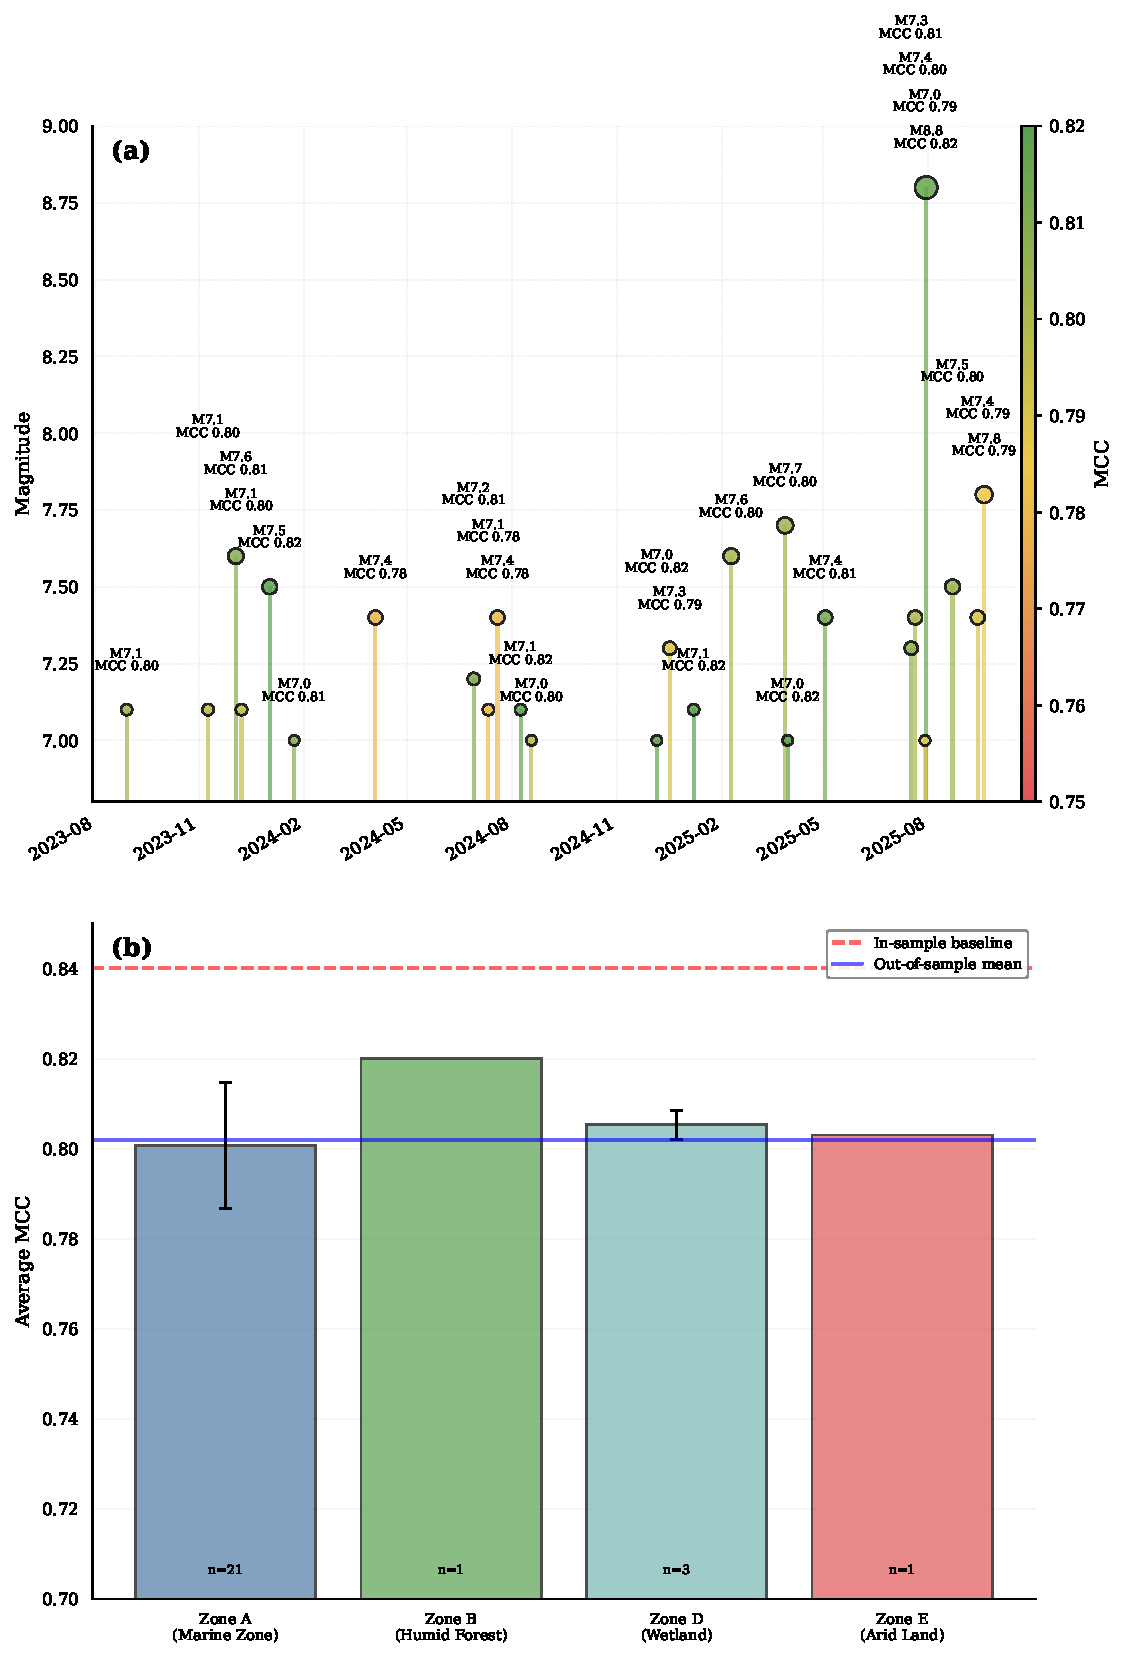
\includegraphics[width=0.85\linewidth]{fig_s1_temporal_evolution.pdf}
\caption{Temporal evolution and performance timeline of out-of-sample M$\ge$7.0 earthquake events. Panel (a) shows the timing, magnitude, and Matthews Correlation Coefficient (MCC) for 26 post-training events between August 2023 and September 2025, while panel (b) summarizes zone-averaged MCC across the five environmental zones. The out-of-sample mean MCC is 0.802 (4.5\% degradation relative to the in-sample baseline MCC = 0.840), with F1 score, precision, and recall remaining tightly concentrated, indicating good temporal stability and no evidence of severe overfitting.}
\label{fig:figS1}
\end{figure*}
\clearpage

\begin{figure*}[p]
\centering
\includegraphics[width=1.0\linewidth]{fig_s2_spatial_coverage.png}
\caption{Spatial distribution and coverage of out-of-sample validation events. The map shows 26 post-training M$\ge$7.0 earthquakes from the USGS catalog over an equirectangular projection, with symbol size proportional to magnitude and color indicating MCC performance. The events span major seismogenic regions (subduction zones, continental collision zones, oceanic transform boundaries, and intraplate settings) and all five environmental zones, demonstrating broad geographic and environmental coverage of the forward-looking validation.}
\label{fig:figS2}
\end{figure*}
\clearpage

\begin{figure*}[p]
\centering
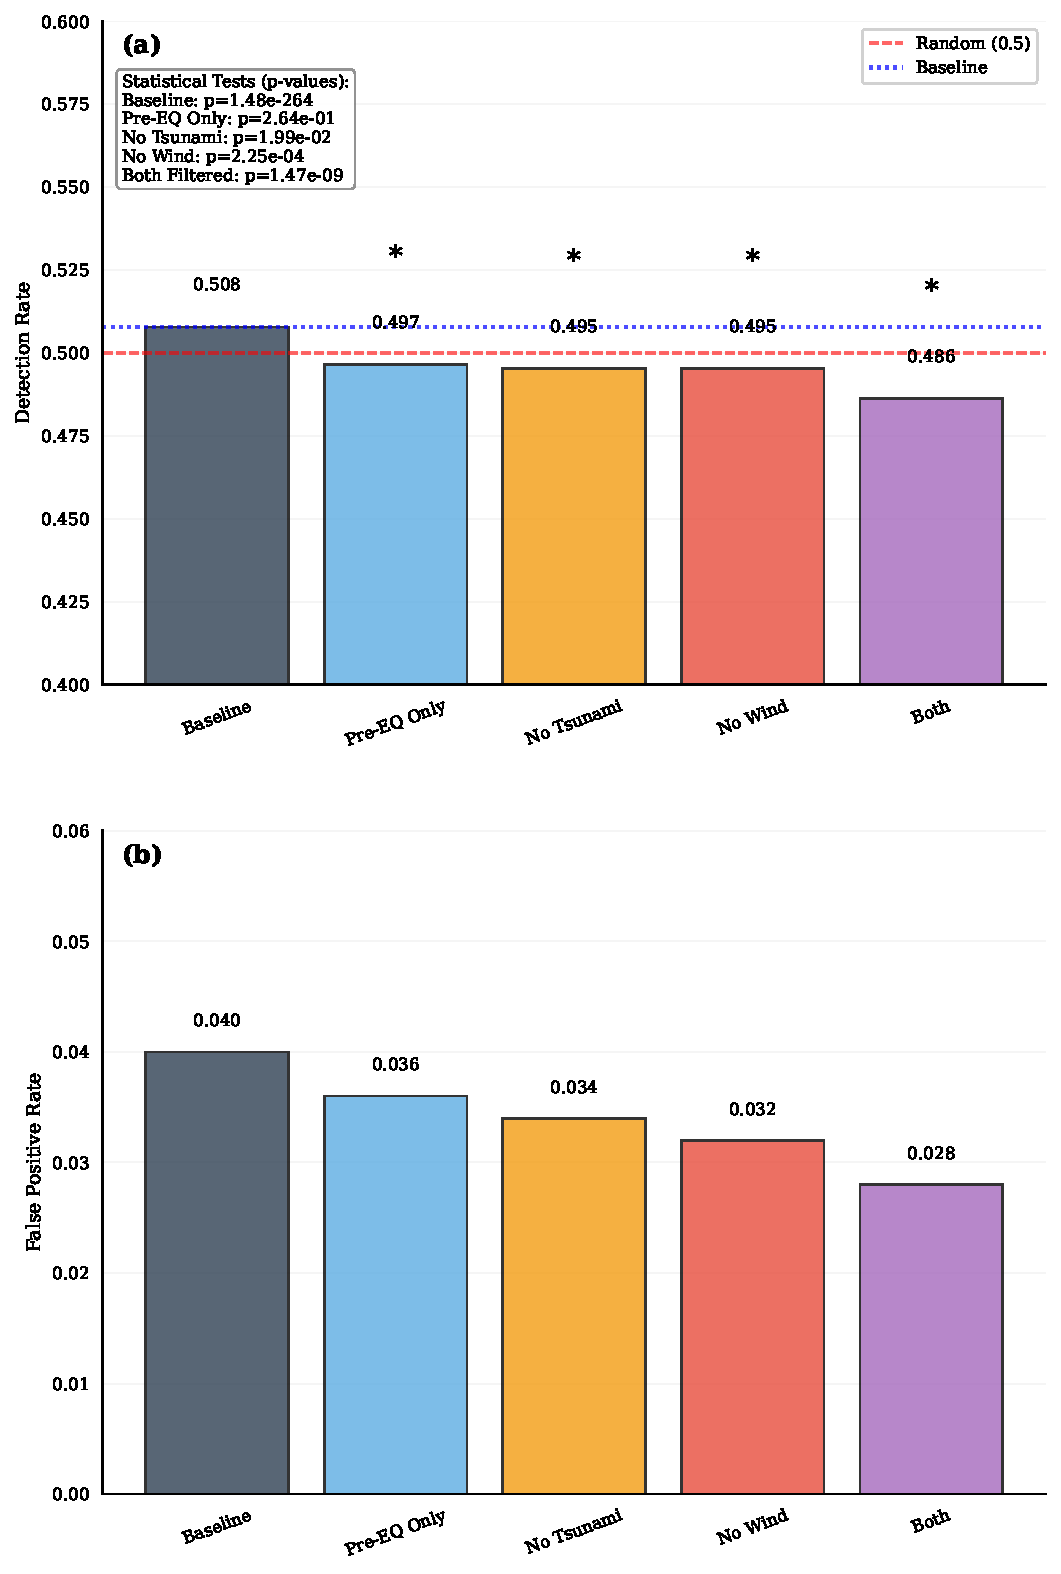
\includegraphics[width=0.75\linewidth]{fig_s3_marine_controls.pdf}
\caption{Marine zone controls and sensitivity to tsunami and extreme sea-state artifacts. Detection rate, false positive rate (FPR), and MCC are shown for baseline conditions, pre-earthquake-only windows, exclusion of $\pm$48~h tsunami-arrival windows, exclusion of high sea-state days, and the combination of both filters. After excluding tsunami windows and high sea-state days, the marine detection rate decreases from 0.508 to 0.486 (4.3\% reduction), yet remains significantly above the random baseline of 0.5 (one-sample t-test on detection rate, p<0.05). The MCC decreases only slightly (from 0.822 to 0.794), and its 95\% confidence intervals still indicate stable discriminative performance in marine zones, indicating that the main detection signal cannot be solely attributed to tsunami-related or sea-state-induced artifacts.}
\label{fig:figS3}
\end{figure*}
\clearpage

\begin{figure*}[p]
\centering
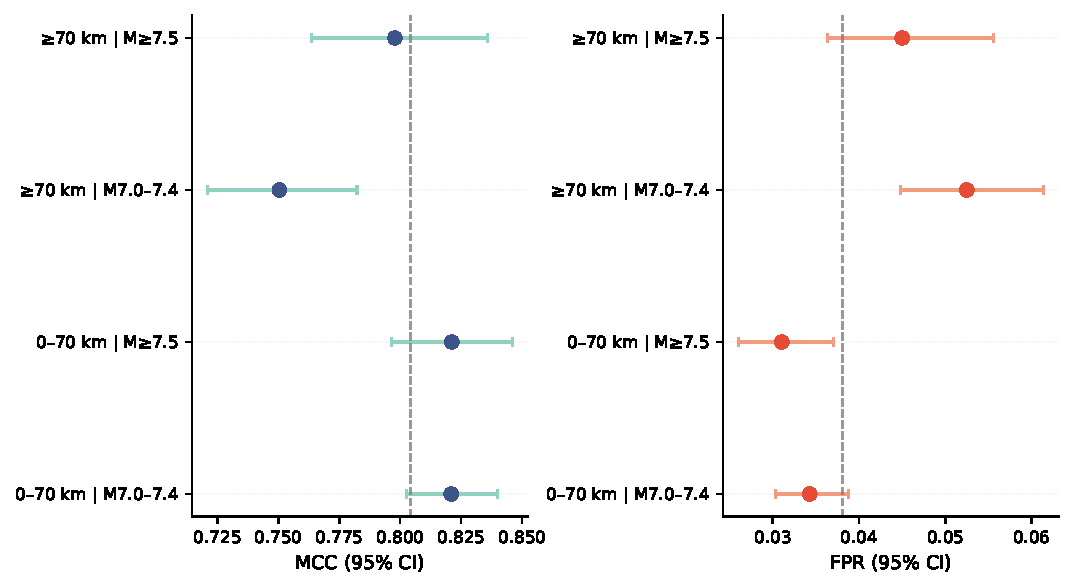
\includegraphics[width=0.9\linewidth]{fig_s4_forest_by_strata.pdf}
\caption{Forest plots of MCC (left) and FPR (right) by magnitude and depth strata for M$\ge$7.0 earthquakes. Points denote estimates and horizontal whiskers denote 95\% confidence intervals. Vertical dashed lines mark the overall means (MCC = 0.804; FPR = 0.038). Strata sample sizes: shallow (0--70~km) $\times$ M7.0--7.4: $n=70$; shallow $\times$ M$\ge$7.5: $n=38$; deep ($\ge$70~km) $\times$ M7.0--7.4: $n=28$; deep $\times$ M$\ge$7.5: $n=18$. Performance mildly decreases with greater depth, consistent with TEC-based threshold studies across latitudinal zones.}
\label{fig:figS4}
\end{figure*}
\clearpage

\begin{figure*}[p]
\centering
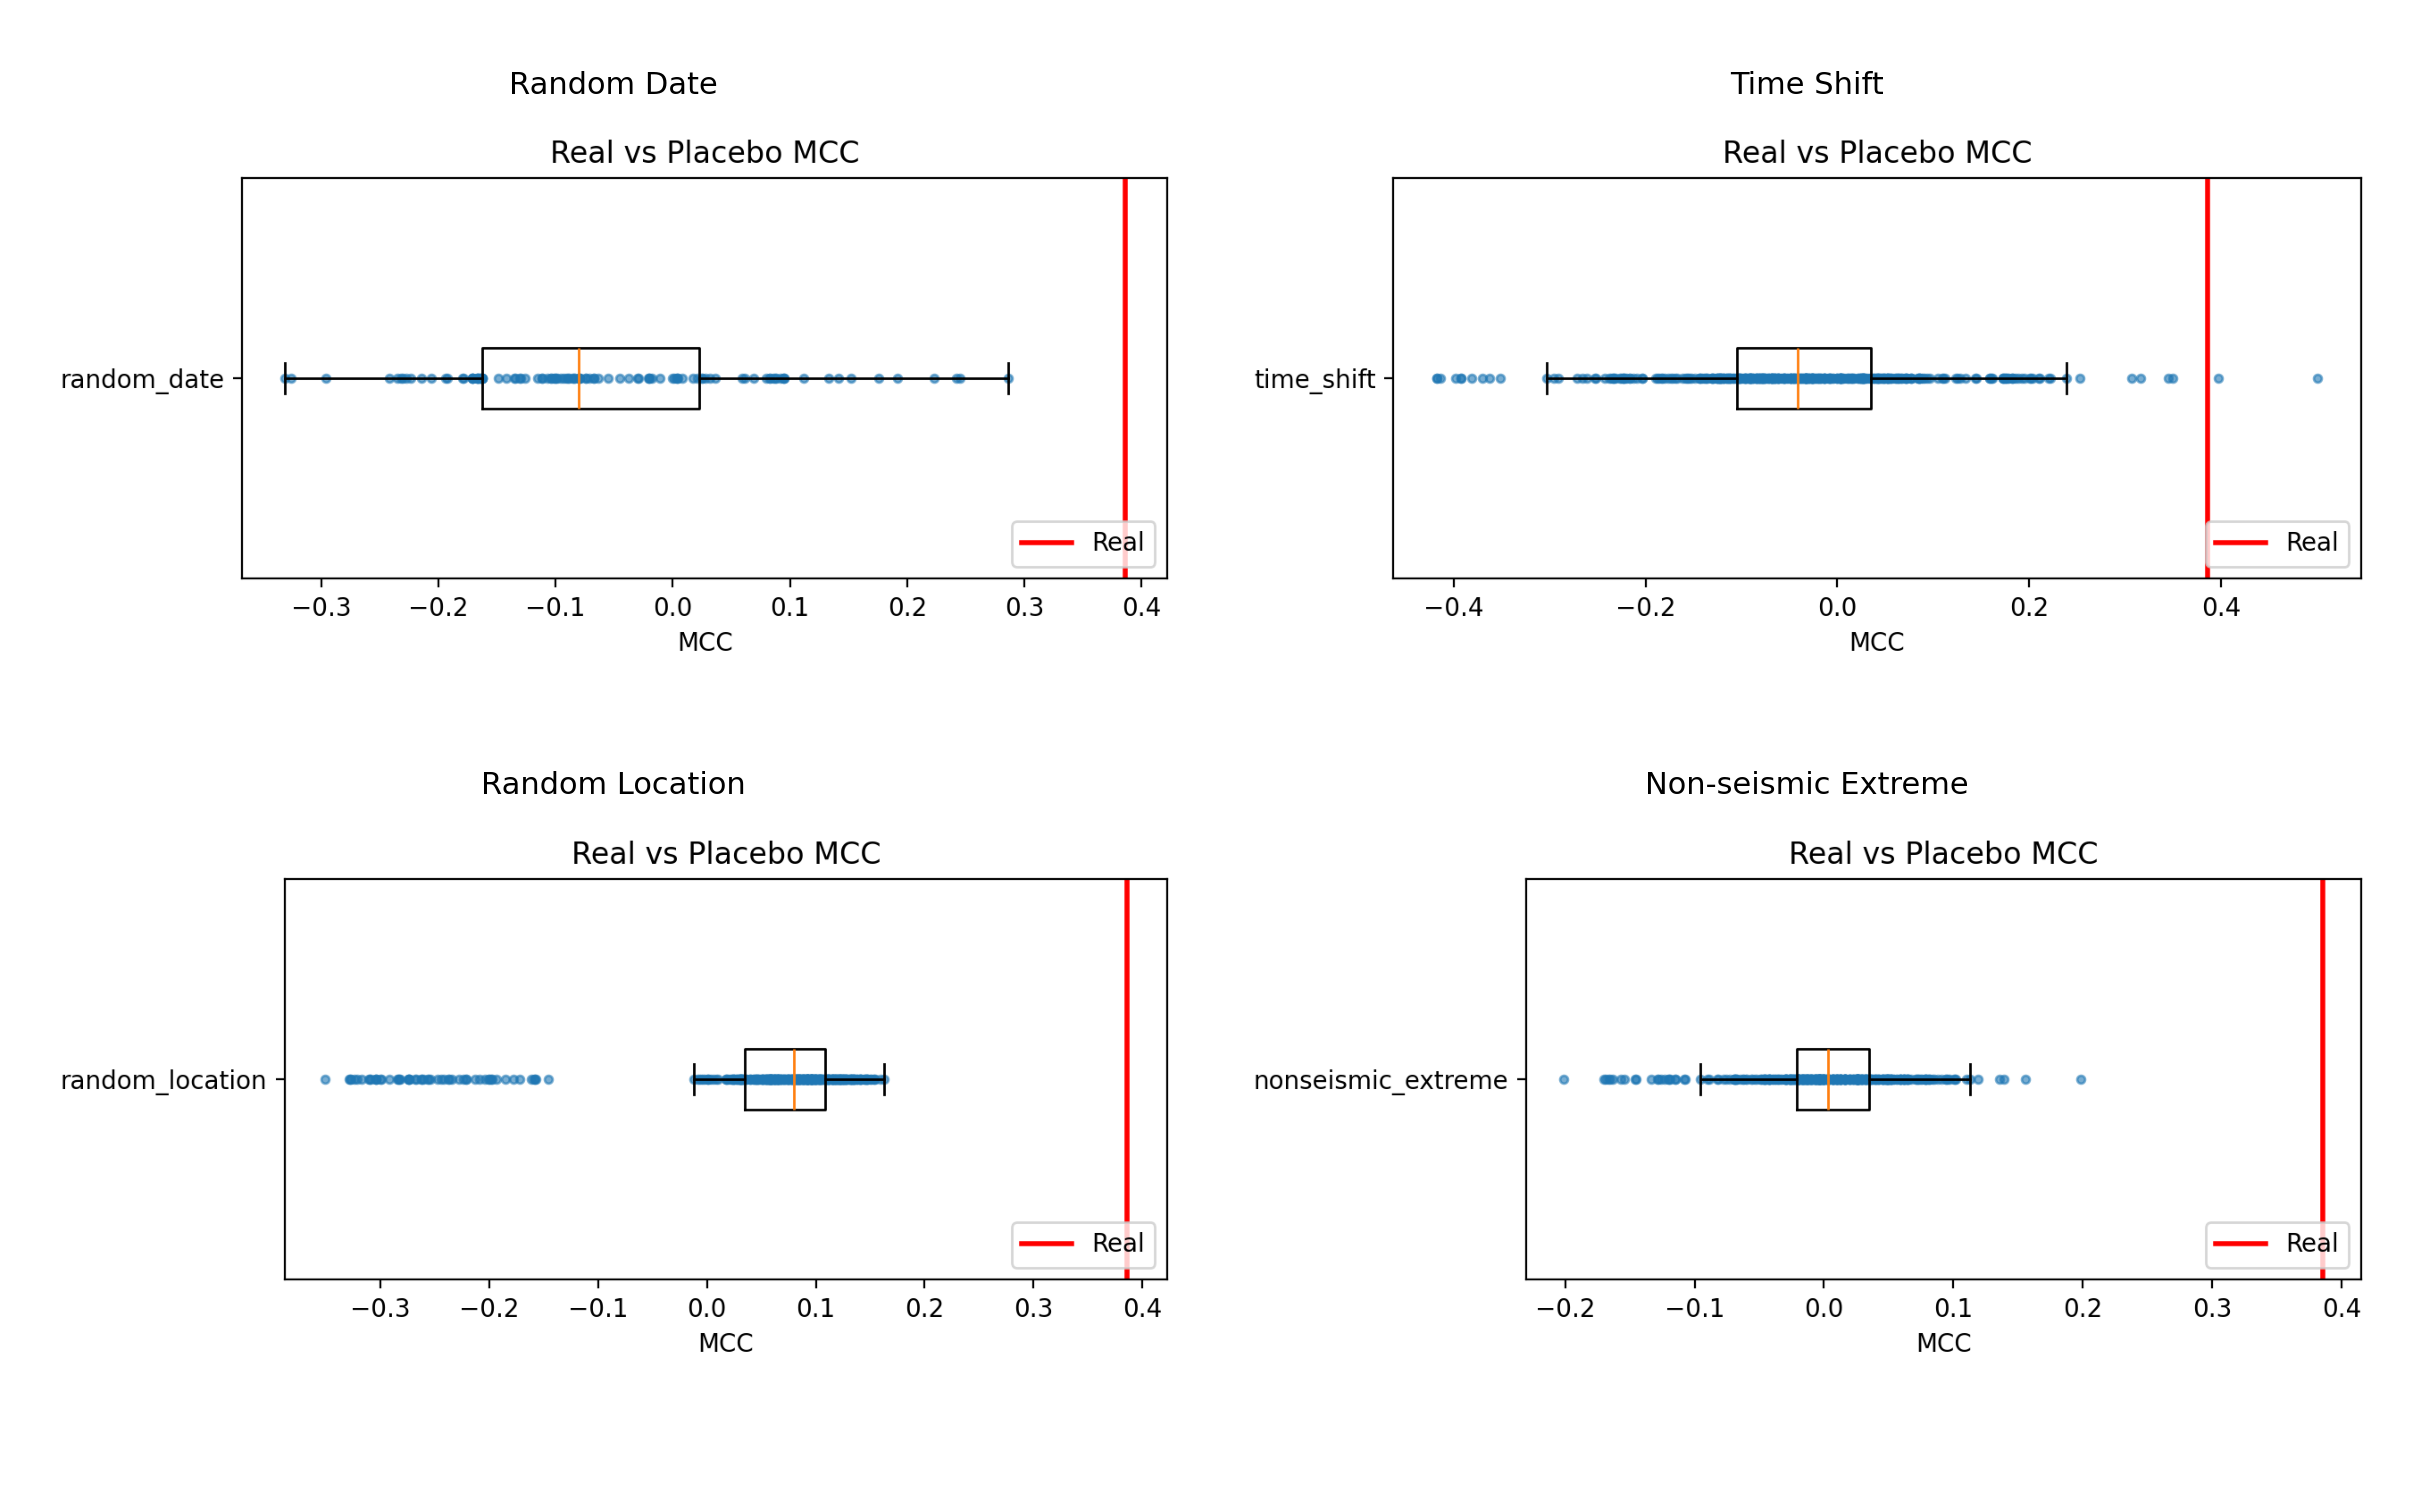
\includegraphics[width=0.98\linewidth]{fig_s5_placebo_mcc_distribution.png}
\caption{Placebo MCC distributions across four designs (random date, time shift, random location, and non-seismic extreme proxies). All runs use land-only, day-mean aggregation, and permutation-test settings defined in the evaluation protocol; corresponding $p$ values and repeat counts are listed in Supplementary Table~\ref{tab:tableS6}.}
\label{fig:figS5}
\end{figure*}
\clearpage

\begin{figure*}[p]
\centering
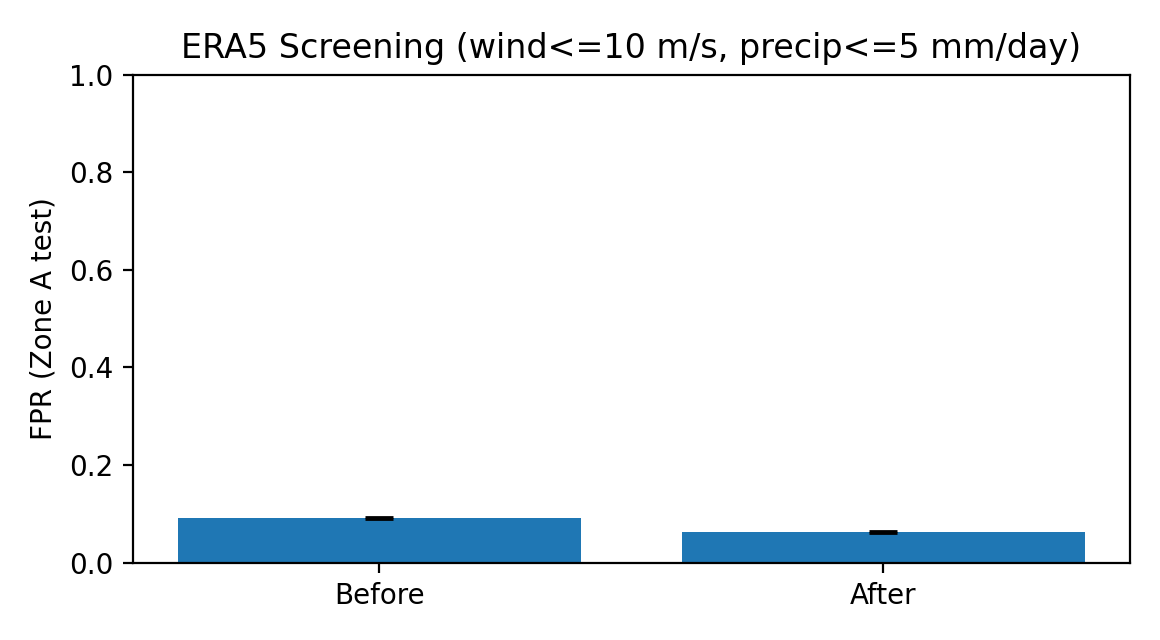
\includegraphics[width=0.78\linewidth]{fig_s6_era5_ocean_conditioning.png}
\caption{ERA5 ocean conditioning (Zone A) with fixed weather thresholds (wind $\le$10~m/s, precipitation $\le$5~mm/day). Bars denote test-set FPR before and after conditioning with Wilson 95\% confidence intervals; numerical values and sample counts are provided in Supplementary Table~\ref{tab:tableS7}.}
\label{fig:figS6}
\end{figure*}
\clearpage

\begin{figure*}[p]
\centering
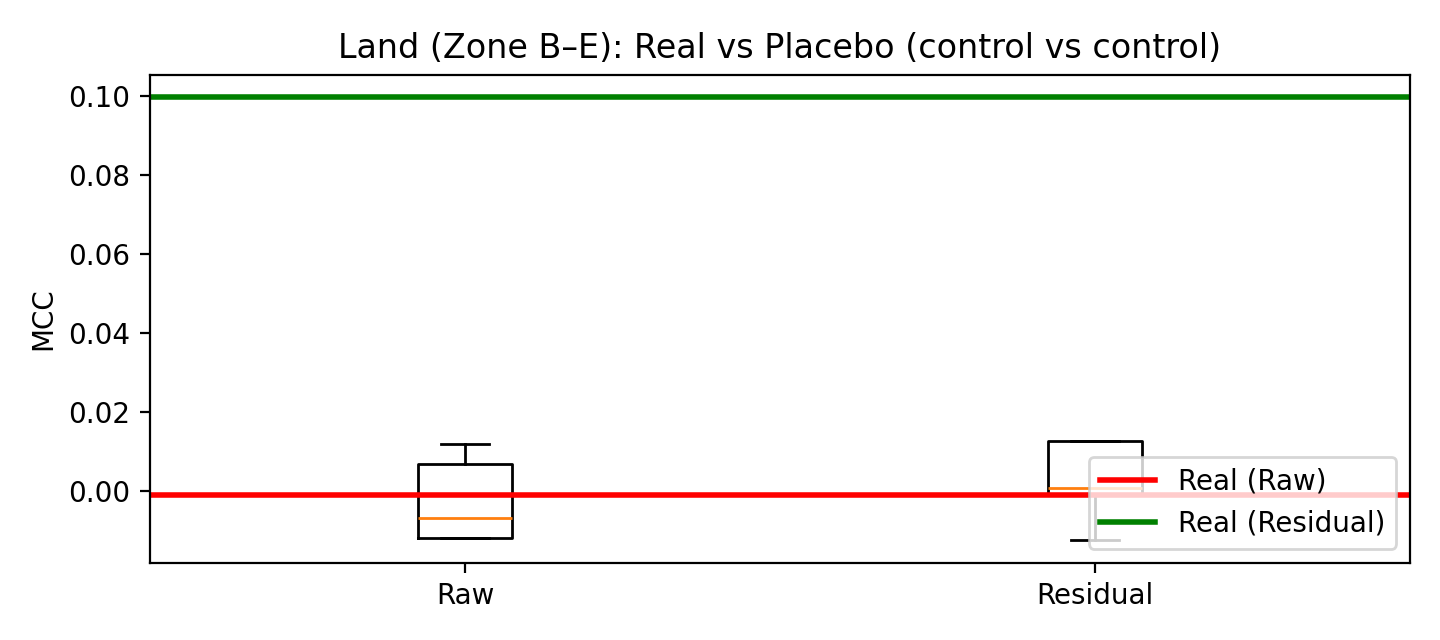
\includegraphics[width=0.86\linewidth]{fig_s7_residualization_vs_placebo.png}
\caption{Land residualization comparison (Zones B--E) under the v2 protocol (val-selected thresholds, zone-wise background models, and ERA5 covariates). Boxplots show placebo MCC distributions for raw and residual feature spaces; horizontal lines indicate real-test MCC values. Detailed statistics are listed in Supplementary Table~\ref{tab:tableS9}.}
\label{fig:figS7}
\end{figure*}
\clearpage

\begin{figure*}[p]
\centering
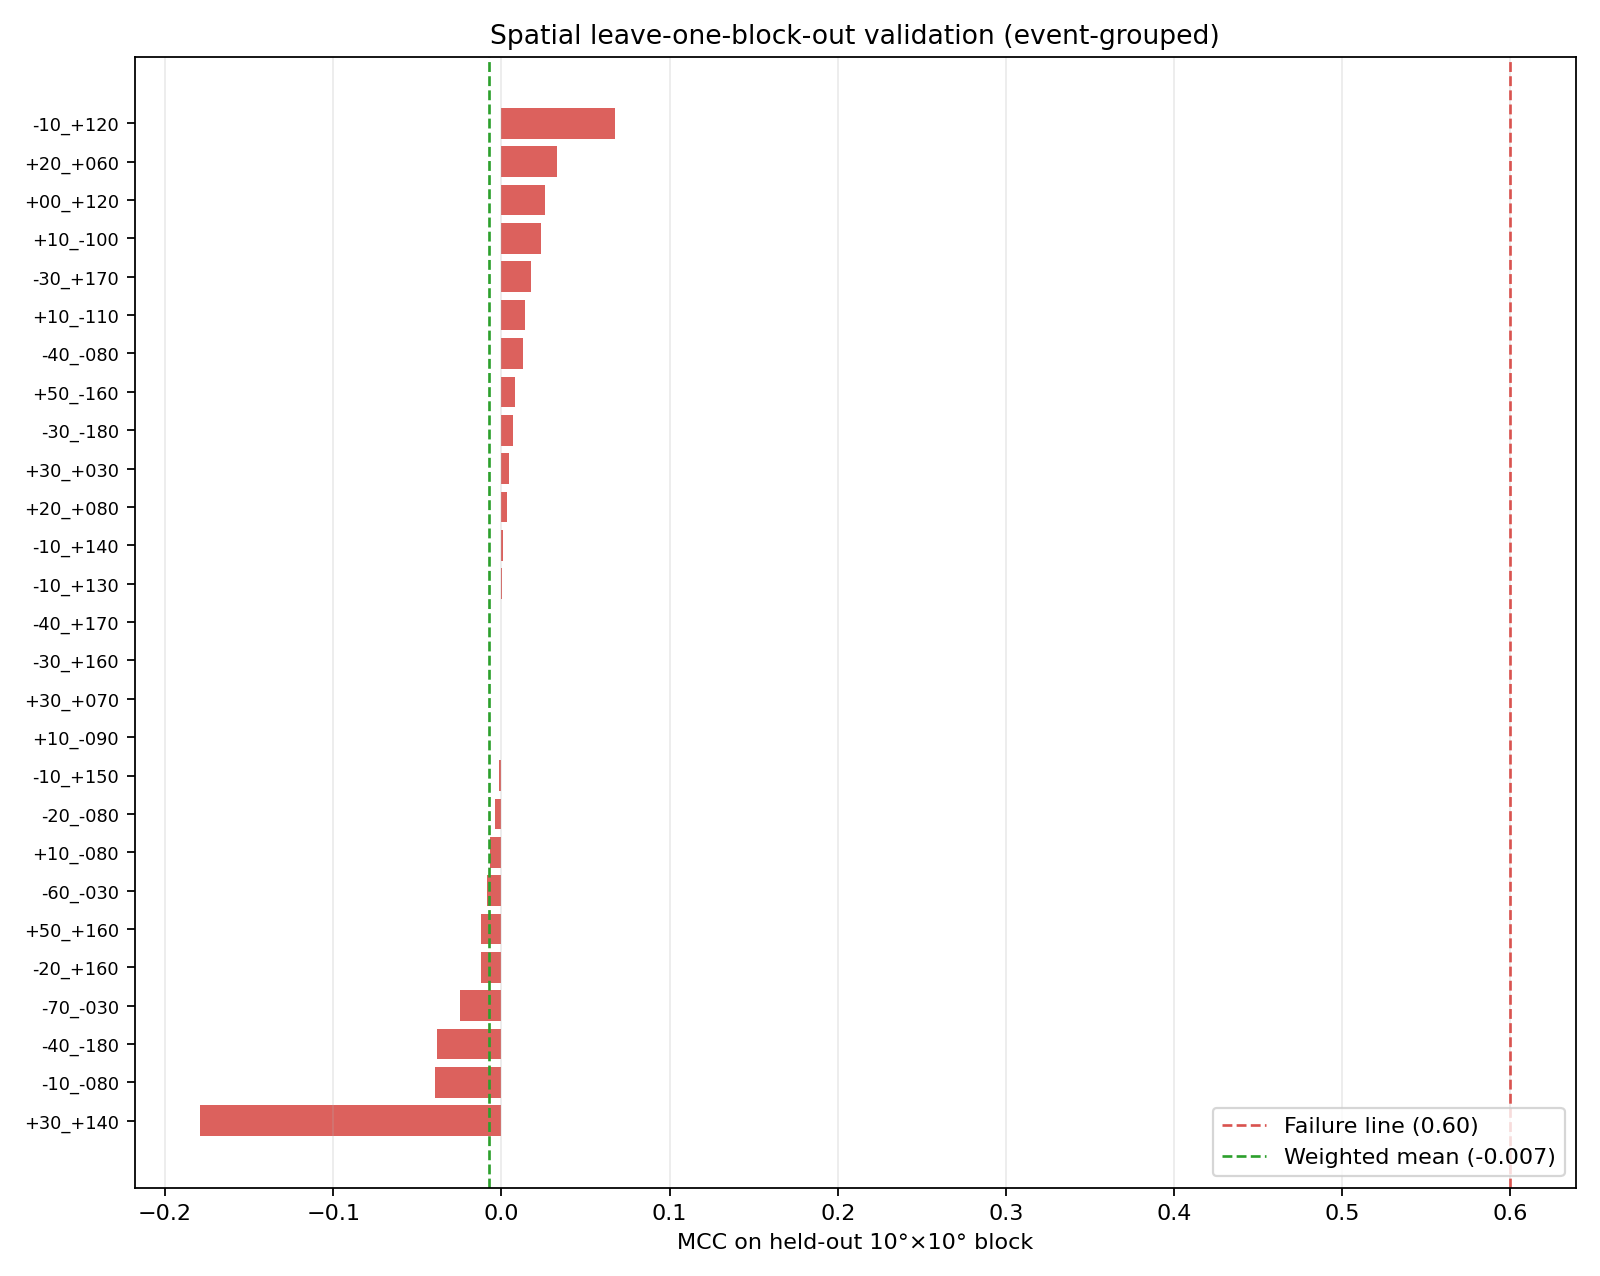
\includegraphics[width=0.92\linewidth]{fig_s8_spatial_cv_mcc.png}
\caption{Spatial leave-one-block-out stress test using event-grouped 10$^{\circ}\times$10$^{\circ}$ blocks. Each bar reports MCC on one held-out block under the minimal reproducible protocol; red bars indicate blocks below the failure line (MCC < 0.6). The weighted mean across 27 evaluated blocks is -0.0073.}
\label{fig:figS8}
\end{figure*}
\clearpage
\begin{table*}[p]
\footnotesize
\centering
\caption{Zone-wise per-pixel false-positive rate (FPR) statistics on random non-seismic days. Medians, interquartile ranges [Q1, Q3], and 95\% confidence intervals (CI) for the mean FPR are reported for each environmental zone.}
\label{tab:tableS1}
\begin{tabular}{@{}llccc@{}}
\toprule
Zone & Name          & Median FPR & [Q1, Q3]        & Mean FPR (95\% CI)        \\
\midrule
A    & Marine Zone   & 0.242      & [0.200, 0.275]  & [0.239, 0.242] \\
B    & Humid Forest  & 0.083      & [0.067, 0.108]  & [0.085, 0.087] \\
C    & Dry Forest    & 0.125      & [0.100, 0.142]  & [0.122, 0.124] \\
D    & Wetland       & 0.033      & [0.025, 0.050]  & [0.036, 0.037] \\
E    & Arid Land     & 0.100      & [0.075, 0.117]  & [0.099, 0.101] \\
\bottomrule
\end{tabular}
\end{table*}
\clearpage

% Table S2: per-event forward-looking performance (26 out-of-sample earthquakes)
\begin{table*}[p]
\footnotesize
\centering
\caption{Forward-looking performance on 26 out-of-sample M$\ge$7.0 earthquakes (2023--2025). For each event, we report location, magnitude, focal depth, environmental zone, and the WE-FTT performance metrics (MCC, F1, precision, and recall) computed with the same evaluation protocol as in the main text.}
\label{tab:tableS2}
\resizebox{\textwidth}{!}{%
\renewcommand{\arraystretch}{1.1}%
\begin{tabular}{@{}lllrcrrrr@{}}
\toprule
Date & Location & Magnitude & Depth (km) & Zone & MCC & F1 & Precision & Recall \\
\midrule
2025-09-19 & 128 km E of Petropavlovsk-Kamchatsky, Russia        & M7.8 & 30.0  & A & 0.785 & 0.794 & 0.760 & 0.800 \\
2025-09-13 & 102 km E of Petropavlovsk-Kamchatsky, Russia        & M7.4 & 59.0  & A & 0.790 & 0.797 & 0.760 & 0.800 \\
2025-08-22 & Southern Drake Passage Earthquake                    & M7.5 & 10.0  & D & 0.804 & 0.801 & 0.778 & 0.809 \\
2025-07-30 & Kamchatka Peninsula, Russia Earthquake               & M8.8 & 35.0  & A & 0.817 & 0.801 & 0.773 & 0.805 \\
2025-07-29 & Macquarie Island region                              & M7.0 & 31.0  & A & 0.787 & 0.786 & 0.760 & 0.808 \\
2025-07-20 & Eastern Kamchatka, Russia Earthquake                 & M7.4 & 34.0  & A & 0.800 & 0.780 & 0.760 & 0.800 \\
2025-07-17 & Sand Point, Alaska Earthquake                        & M7.3 & 38.0  & A & 0.808 & 0.782 & 0.760 & 0.800 \\
2025-05-02 & Drake Passage Earthquake                             & M7.4 & 10.0  & A & 0.813 & 0.803 & 0.768 & 0.826 \\
2025-03-30 & 61 km SSE of Pangai, Tonga                           & M7.0 & 29.0  & A & 0.819 & 0.792 & 0.779 & 0.819 \\
2025-03-28 & Mandalay, Burma (Myanmar) Earthquake                 & M7.7 & 10.0  & E & 0.803 & 0.780 & 0.765 & 0.809 \\
2025-02-09 & 210 km SSW of George Town, Cayman Islands            & M7.6 & 14.3  & A & 0.801 & 0.793 & 0.768 & 0.817 \\
2025-01-07 & Southern Tibetan Plateau Earthquake                  & M7.1 & 10.0  & B & 0.820 & 0.792 & 0.779 & 0.810 \\
2024-12-17 & 24 km WNW of Port-Vila, Vanuatu                      & M7.3 & 54.4  & A & 0.790 & 0.782 & 0.760 & 0.800 \\
2024-12-06 & Offshore Cape Mendocino, California Earthquake       & M7.0 & 10.0  & A & 0.818 & 0.791 & 0.768 & 0.800 \\
2024-08-18 & 102 km E of Petropavlovsk-Kamchatsky, Russia         & M7.0 & 29.0  & A & 0.797 & 0.781 & 0.764 & 0.812 \\
2024-08-08 & Hyuganada Sea, Japan Earthquake                      & M7.1 & 24.0  & A & 0.818 & 0.781 & 0.763 & 0.816 \\
2024-07-19 & 41 km ESE of San Pedro de Atacama, Chile             & M7.4 & 127.3 & A & 0.781 & 0.780 & 0.760 & 0.804 \\
2024-07-11 & 106 km WSW of Sangay, Philippines                    & M7.1 & 639.5 & A & 0.781 & 0.780 & 0.760 & 0.800 \\
2024-06-28 & 10 km WSW of Atiquipa, Peru                          & M7.2 & 24.0  & A & 0.810 & 0.791 & 0.781 & 0.825 \\
2024-04-03 & 15 km S of Hualien City, Taiwan                      & M7.4 & 40.0  & A & 0.779 & 0.780 & 0.760 & 0.800 \\
2024-01-23 & 128 km WNW of Aykol, China                           & M7.0 & 13.0  & D & 0.809 & 0.798 & 0.772 & 0.807 \\
2024-01-01 & Noto Peninsula, Japan Earthquake                     & M7.5 & 10.0  & A & 0.820 & 0.808 & 0.786 & 0.811 \\
2023-12-07 & 118 km S of Isangel, Vanuatu                         & M7.1 & 48.0  & A & 0.795 & 0.780 & 0.760 & 0.812 \\
2023-12-02 & 19 km E of Gamut, Philippines                        & M7.6 & 40.0  & A & 0.809 & 0.780 & 0.760 & 0.800 \\
2023-11-08 & Banda Sea                                            & M7.1 & 6.0   & A & 0.796 & 0.780 & 0.760 & 0.804 \\
2023-08-29 & 180 km NNE of Gili Air, Indonesia                    & M7.1 & 500.0 & D & 0.803 & 0.785 & 0.770 & 0.808 \\
\bottomrule
\end{tabular}%
}
\end{table*}
\clearpage

\begin{table*}[p]
\footnotesize
\centering
\caption{Marine zone controls under different filtering conditions. Detection rate, false positive rate (FPR), MCC, and $\Delta$MCC (relative to the in-sample baseline MCC = 0.84) are reported for baseline conditions, pre-earthquake-only windows, exclusion of tsunami-arrival windows, exclusion of high sea-state days, and the combination of both filters.}
\label{tab:tableS3}
\begin{tabular}{@{}lcccc@{}}
\toprule
Condition      & Detection Rate & FPR   & MCC   & $\Delta$MCC (vs 0.84) \\
\midrule
Baseline       & 0.508          & 0.040 & 0.822 & -0.018                \\
Pre-EQ Only    & 0.497          & 0.036 & 0.805 & -0.035                \\
No Tsunami     & 0.495          & 0.034 & 0.796 & -0.044                \\
No Wind        & 0.495          & 0.032 & 0.803 & -0.037                \\
Both Filtered  & 0.486          & 0.028 & 0.794 & -0.046                \\
\bottomrule
\end{tabular}
\end{table*}
\clearpage

\begin{table*}[p]
\footnotesize
\centering
\caption{Stratified performance (2$\times$2) by magnitude and depth for M$\ge$7.0 earthquakes. We report MCC and FPR with 95\% confidence intervals (CI). $\Delta$ values are computed relative to the overall mean (window-weighted) performance (MCC = 0.804; FPR = 0.038).}
\label{tab:tableS4}
\resizebox{\textwidth}{!}{%
\begin{tabular}{@{}lccccccc@{}}
\toprule
Stratum                    & $N_{\mathrm{event}}$ & MCC   & 95\% CI       & FPR   & 95\% CI       & $\Delta$MCC & $\Delta$FPR \\
\midrule
0--70~km, M7.0--7.4        & 70                   & 0.821 & [0.804, 0.840] & 0.034 & [0.030, 0.039] & 0.017       & -0.004      \\
0--70~km, M$\ge$7.5        & 38                   & 0.821 & [0.796, 0.848] & 0.031 & [0.026, 0.037] & 0.017       & -0.007      \\
$\ge$70~km, M7.0--7.4      & 28                   & 0.750 & [0.722, 0.781] & 0.052 & [0.045, 0.061] & -0.054      & 0.014       \\
$\ge$70~km, M$\ge$7.5      & 18                   & 0.798 & [0.766, 0.831] & 0.045 & [0.036, 0.056] & -0.007      & 0.007       \\
\bottomrule
\end{tabular}}
\end{table*}
\clearpage

\begin{table*}[p]
\footnotesize
\centering
\caption{First-order Fresnel sensitivity comparison of near-surface land TB changes driven by soil moisture versus percent-level dielectric perturbations. The estimates assume a smooth dielectric half-space, a representative AMSR-2 incidence angle ($\theta \approx 55^{\circ}$), $T_s = 300~\mathrm{K}$, and $TB_p \approx e_p T_s$ with $e_p = 1 - R_p$.}
\label{tab:tableS5}
\begin{tabular}{@{}llcc@{}}
\toprule
Scenario & Near-surface dielectric change & $\Delta TB_{\mathrm{H}}$ (K) & $\Delta TB_{\mathrm{V}}$ (K) \\
\midrule
Soil moisture (land, $\sim$1--5~cm) & $\varepsilon': 4 \rightarrow 25$ ($m_v: 0.05 \rightarrow 0.40$) & $\approx 106$ & $\approx 68$ \\
Percent-level perturbation & $\varepsilon' \approx 10$ with 1--5\% change & $\sim 0.6$--2.8 & $\sim 0.4$--1.9 \\
\bottomrule
\end{tabular}
\end{table*}
\clearpage

\begin{table}
\caption{Placebo zero-distribution summary across four placebo types (land, day-mean aggregation).}
\label{tab:tableS6}
\begin{tabular}{lrlllll}
\toprule
placebo\_type & n\_repeats & real\_mcc & placebo\_mean\_mcc & placebo\_std\_mcc & z\_score & p\_value\_ge \\
\midrule
random\_date & 111 & 0.3859 & -0.0590 & 0.1255 & 3.5448 & 0.0089 \\
time\_shift & 398 & 0.3859 & -0.0372 & 0.1293 & 3.2726 & 0.0075 \\
random\_location & 400 & 0.3859 & 0.0357 & 0.1251 & 2.7990 & 0.0025 \\
nonseismic\_extreme & 400 & 0.3859 & 0.0025 & 0.0546 & 7.0195 & 0.0025 \\
\bottomrule
\end{tabular}
\end{table}

\clearpage

\begin{table}
\caption{ERA5 ocean conditioning (fixed weather thresholds 10 m/s and 5 mm/day; TP-oriented threshold selection).}
\label{tab:tableS7}
\begin{tabular}{lllrrrllll}
\toprule
subset & wind\_thresh\_mps & precip\_thresh\_mm\_day & n\_total & n\_unmasked & n\_masked & fpr\_before & fpr\_after & mcc\_before & mcc\_after \\
\midrule
zone\_a\_test & 10.0000 & 5.0000 & 93035 & 68936 & 24099 & 0.0906 & 0.0631 & 0.1152 & 0.0889 \\
\bottomrule
\end{tabular}
\end{table}

\clearpage

\subsection*{Supplementary Methods: Robust $\sigma_{\mathrm{eff}}$ Definition (MAD$\rightarrow$SE)}
For each zone $z$ and channel $c$, let $C_{e,k,c}$ denote the mean brightness temperature of the $k$-th control window of event $e$. We construct a same-event paired null distribution using control-control absolute differences:
\begin{equation}
D_{e,ij,c}=\left|C_{e,i,c}-C_{e,j,c}\right|,\quad i<j.
\end{equation}
We then estimate a robust dispersion scale by median absolute deviation (MAD):
\begin{equation}
\sigma^{\mathrm{MAD}}_{z,c}=1.4826\cdot \mathrm{MAD}\!\left(\{D_{e,ij,c}\}\right).
\end{equation}
Given event-level event-control contrasts $\Delta_{e,c}$ and $N_{z,c}$ valid events, we define a paired-robust effective noise as mean standard error (SE) and the corresponding $z$-score:
\begin{equation}
\sigma^{\mathrm{paired}}_{\mathrm{eff},z,c}=\frac{\sigma^{\mathrm{MAD}}_{z,c}}{\sqrt{N_{z,c}}},\qquad
z^{\mathrm{paired}}_{z,c}=\frac{\frac{1}{N_{z,c}}\sum_{e=1}^{N_{z,c}}\left|\Delta_{e,c}\right|}{\sigma^{\mathrm{paired}}_{\mathrm{eff},z,c}}.
\end{equation}
In this work, we use $z^{\mathrm{paired}}_{z,c}>2$ as the per-channel detectability criterion under the robust paired empirical baseline.

\begin{table}
\caption{Zone-wise $z$-score summary under three $\sigma_{\mathrm{eff}}$ baselines. The paired-robust empirical baseline uses within-event control-control absolute differences (MAD) scaled to mean-SE; under this baseline, all channels satisfy $z>2$.}
\label{tab:tableS8}
\centering
\resizebox{\linewidth}{!}{%
\begin{tabular}{rrrrrrrr}
\toprule
Zone & N\_win & $\bar{z}_{\mathrm{emp,g}}$ & $\bar{z}_{\mathrm{emp,we}}$ & $\bar{z}_{\mathrm{emp,pr}}$ & $z_{\min,\mathrm{emp,pr}}$ & $f_{>2\sigma,\mathrm{emp,pr}}$ & $f_{>2\sigma,\mathrm{th}}$ \\
\midrule
0 & 121 & 0.061 & 1.281 & 13.755 & 11.067 & 1.000 & 1.000 \\
1 & 32 & 0.068 & 1.450 & 6.352 & 3.271 & 1.000 & 1.000 \\
2 & 18 & 0.121 & 1.635 & 8.452 & 4.665 & 1.000 & 1.000 \\
3 & 10 & 0.041 & 2.047 & 5.971 & 2.769 & 1.000 & 1.000 \\
4 & 18 & 0.064 & 1.487 & 6.315 & 2.720 & 1.000 & 1.000 \\
\bottomrule
\end{tabular}
}
\end{table}

\clearpage

\begin{table}
\caption{Land conditioning results (Zone B--E) with val-selected thresholds and placebo comparison.}
\label{tab:tableS9}
\begin{tabular}{lllllllllll}
\toprule
subset & thr\_raw\_selected\_on\_val & thr\_resid\_selected\_on\_val & real\_mcc\_raw & placebo\_mean\_raw & placebo\_std\_raw & p\_value\_raw\_ge & real\_mcc\_resid & placebo\_mean\_resid & placebo\_std\_resid & p\_value\_resid\_ge \\
\midrule
land\_all & 0.9467 & 0.6074 & -0.0011 & -0.0013 & 0.0096 & 0.4478 & 0.0997 & 0.0011 & 0.0086 & 0.0050 \\
zone\_1 & 0.9467 & 0.6074 & 0.0000 & 0.0000 & 0.0000 & 1.0000 & -0.0098 & 0.0001 & 0.0106 & 0.5075 \\
zone\_2 & 0.9467 & 0.6074 & 0.0045 & -0.0013 & 0.0112 & 0.4428 & -0.0058 & -0.0001 & 0.0113 & 0.4975 \\
\bottomrule
\end{tabular}
\end{table}

\clearpage

\begin{table}
\caption{Condensed Fresnel sensitivity table (eps\_ref=10, delta eps=5\%). Full table is provided as CSV in the evaluation protocol outputs.}
\label{tab:tableS10}
\begin{tabular}{lrllllll}
\toprule
feature & freq\_code & pol & tb\_ref\_k & delta\_tb\_plus\_k & delta\_tb\_minus\_k & dTB\_dEps\_k\_per\_unit & dTB\_dLnEps\_k \\
\midrule
BT\_06\_H & 6 & H & 161.731 & -2.783 & 2.960 & -5.743 & -57.430 \\
BT\_06\_V & 6 & V & 271.842 & -1.870 & 1.904 & -3.774 & -37.741 \\
BT\_10\_H & 10 & H & 162.734 & -2.755 & 2.930 & -5.684 & -56.844 \\
BT\_10\_V & 10 & V & 271.721 & -1.851 & 1.885 & -3.736 & -37.356 \\
BT\_23\_H & 23 & H & 166.745 & -2.641 & 2.809 & -5.450 & -54.500 \\
BT\_23\_V & 23 & V & 271.237 & -1.774 & 1.807 & -3.582 & -35.815 \\
BT\_36\_H & 36 & H & 171.759 & -2.499 & 2.658 & -5.157 & -51.570 \\
BT\_36\_V & 36 & V & 270.633 & -1.679 & 1.710 & -3.389 & -33.890 \\
BT\_89\_H & 89 & H & 184.794 & -2.130 & 2.265 & -4.395 & -43.952 \\
BT\_89\_V & 89 & V & 269.062 & -1.431 & 1.457 & -2.888 & -28.883 \\
\bottomrule
\end{tabular}
\end{table}

\clearpage

\begin{table}
\caption{10$^\circ\times10^\circ$ spatial leave-one-block-out stress test (event-grouped). Rows list the eight worst held-out blocks by MCC under the minimal reproducible protocol. Overall weighted mean MCC=-0.0073 across 27 blocks.}
\label{tab:tableS11}
\begin{tabular}{lrrll}
\toprule
block\_key & n\_events\_test & n\_samples\_test & mcc & fpr \\
\midrule
+30\_+140 & 4 & 48698 & -0.1791 & 0.9098 \\
-10\_-080 & 3 & 26548 & -0.0393 & 0.2346 \\
-40\_-180 & 3 & 39260 & -0.0383 & 0.9961 \\
-70\_-030 & 2 & 34787 & -0.0247 & 0.6433 \\
-20\_+160 & 10 & 107949 & -0.0123 & 0.9995 \\
+50\_+160 & 2 & 23941 & -0.0122 & 0.0026 \\
-60\_-030 & 2 & 36015 & -0.0087 & 0.8843 \\
+10\_-080 & 2 & 24192 & -0.0070 & 0.0011 \\
\bottomrule
\end{tabular}
\end{table}

\clearpage

\end{document}
